\documentclass[a4paper,11pt]{thesis}

\usepackage{amsmath}
\usepackage{amssymb}
\usepackage{graphicx}
\usepackage{makeidx}
\usepackage{theorem}
\usepackage{array}
%\usepackage{booktabs}


\title{Antennas in plasma: numerical calculation}
\author{T.H. Oswald, MSc}

\renewcommand{\baselinestretch}{1.33}
\begin{document}

\maketitle

\newpage
\paragraph*{}
 \begin{verbatim}












\end{verbatim}
\begin{center}
\framebox{\parbox[c]{12cm}{
\begin{center}
\emph{This thesis is dedicated to my parents.}
\end{center}
}}
\end{center}
\frontmatter
\chapter{\textbf{Acknowledgments}}
Many people were involved in the successful creation of this thesis. Above all I thank Prof. H.O. Rucker who offered me to work on this subject and supported me with his great experience. I also thank my colleague W. Macher and who never ran out of patience when I attacked him with countless questions. I am also deeply indebted to my wife Mary and my children Michael, Anja, and Viktoria who provided me with the necessary time to complete this task. Last but not least, I thank my parents, without whom this document would not exist in many respects.

\tableofcontents
%\begin{abstract}

%\end{abstract}
\mainmatter
\chapter{Introduction and Objectives}
Remote Sensing is a term that describes the procedure of gathering information remotely. Space science is one of the fields, where remote sensing is used to a very great extent. Due to the hostile environment of space and the large distances involved, it is often the only possible way to extend the knowledge on these distant worlds. Remote sensing, in turn, relies heavily upon the use of electromagnetic radiation and other kinds of plasma waves which are transmitted and received by means of antennas.\\

Antennas can be seen as interface between free-wave propagation and guided wave propagation. When plasma waves are received or excited by means of an antenna, a mode conversion takes place in addition to this. On a spacecraft, there usually exist two types of antennas. The antennas used for communication with Earth are normally parabolic antenna dishes. The behavior of such antennas depends mostly on the shape of the antenna dish and is only to a little extent influenced by the surrounding plasma. This doctoral thesis does not treat such antennas.\\

The second type of antenna often found on spacecraft is the scientific antenna. Scientific antennas, often monopoles, have the task of receiving waves of a natural source. Analysis of the received waves yields information about the physics of the process which generates  these waves.\\

For a correct interpretation of the received data it is mandatory that the reception properties of the antenna are known with high accuracy. There are certain parameters which can be used to describe antenna behavior, like the effective length vectors, antenna impedances and radiation patterns. Unfortunately, the real behavior of the antennas is different than one would predict for the geometric configuration of the antennas. The reason is the influence of the body of the spacecraft as well as the influence of the surrounding space plasma.\\

The spacecraft surface is made of conducting material, so it can, in principle, be regarded as part of the antennas. As a result, each antenna behaves as if it would point into a slightly different direction, with a slightly different length. The vector that describes the direction and length of this virtual antenna is called effective length vector. This effective length vector has to be determined, before any data analysis of the received EM waves can be conducted.\\

The procedure of finding the antenna parameters is called antenna calibration. There are four known methods to determine the effective length vectors of the antennas of a spacecraft:

\begin{enumerate}
\item The numerical approach.
\item The rheometry, an experimental approach.
\item The anechoic chamber, another experimental method.
\item In-flight calibration.
\end{enumerate}

All four methods complement each other and are necessary components of the process of determination and validation of the antenna properties. The content of this doctoral thesis is applicable to the numerical method.\\

There are several numerical methods to simulate a receiving or transmitting antenna. One of the most widely used is the Method of Moments
(MoM), which is exclusively used in this thesis. It is realized by computer programs and consists of two steps. In the first step, the distribution of the currents on the surface of hull and antennas is calculated. This distribution can be used to calculate the effective length vectors and other antenna properties, like antenna impedances. This procedure is the second step.\\

The properties of antennas on spacecraft are also influenced by the space plasma which surrounds the spacecraft. Unlike in vacuum there exist many different wave modes which can propagate through plasma and are received by the antennas. Each wave travels with a different speed and polarization, which makes the analysis extremely difficult. The magnitude of the influence is highest at low frequencies and decreases above the characteristic plasma frequencies. At the typical frequencies of the receivers of radio experiments the influence is small, which is the reason that plasma effects are usually neglected in spacecraft antenna calibration. It will be shown in this PhD thesis that the effects should not be ignored when calibrating spacecraft antennas which operate under certain conditions.\\

The objective of this doctoral thesis is to show how plasma effects can be included into the numerical calibration process. In the following 3 chapters the theoretical framework is established and the necessary equations, which are used in the numerical computations, are derived. Two different methods are used to incorporate the models of space plasma into the calibration.\\

One possibility is to use a dielectric model of plasma and encapsulate it in the so-called dyadic Green's function which is part of the electric field integral equation, which in turn governs the current distribution on the surface of the spacecraft. This method is applied in chapter 5 in combination with a short dipole and in chapter 6 where it is directly applied to the calibration of the antennas of the NASA STEREO spacecraft.\\

The second method is to model the so-called plasma sheath, a boundary zone around the spacecraft which forms due to the interaction of the conducting surface of the spacecraft with the plasma. This method will be applied in chapter 7.\\

Only the simplest models are practically applied in this doctoral thesis. More complicated models should be used in future but the workload of their implementation would be far too large within the frame of the present work, so further studies should be performed in the context of future projects.


\chapter{Electromagnetics: Basics and formalism}
\section{Electromagnetics in free space}
\subsection{Maxwell's equations}
The base of the whole subject of electromagnetism are the Maxwell
equations. In matter they have the following form:

\begin{eqnarray}
\nabla \cdot \mathbf{D}(\mathbf{r},t)&=&\rho(\mathbf{r},t) \label{maxwell1}\\
\nabla \cdot \mathbf{B}(\mathbf{r},t)&=&0 \label{maxwell2} \\
\nabla \times \mathbf{E}(\mathbf{r},t)&=&-\frac{\partial \mathbf{B}(\mathbf{r},t)}{\partial t} \label{maxwell3} \\
\nabla \times \mathbf{H}(\mathbf{r},t)&=&\mathbf{j}(\mathbf{r},t)+ \frac{\partial \mathbf{D}(\mathbf{r},t)}{\partial t} \label{maxwell4}
\end{eqnarray}

The fields are functions of space and time. $\mathbf{j}$ and
$\rho_c$ are the current distribution and charge distribution fields
which are not included in the permittivity. They could alternately
be drawn into the permittivity and/or permeability tensors, which corresponds to the so called dielectric model of the matter which is plasma in the case of space environment.
Additionally the constitutive equations are needed, which relate the
macroscopic fields to the microscopic fields. The general form of the linearized electric constitutive equation is

\begin{equation}
    \mathbf{D}(\mathbf{r},t)=\int_{-\infty,t}\int_V\hat{\epsilon}_{ij}(t,t',\mathbf{r},\mathbf{r'}) E_j(\mathbf{r'},t')d^3\mathbf{r'}dt'
\end{equation}

$\mathbf{\hat{\epsilon}_{ij}}$ are the components of the dielectric tensor. The primed parameters are  variables of integration, which run from minus infinity to t in case of time, and from minus infinity to plus infinity in case of the spatial coordinates. The unprimed parameters denote the point of observation. The entity depends on the history and configuration of each point in space. This phenomenon is called non-locality in space and time. Postulating homogeneity of the medium, the equation can be simplified.

\begin{equation}
    \mathbf{D}(\mathbf{r},t)=\int_{-\infty,t}\int_V\hat{\epsilon}_{ij}(t-t',\mathbf{r}-\mathbf{r'}) E_j(\mathbf{r'},t')d^3\mathbf{r'}dt'
\end{equation}

Performing the Fourier transform and using the results of the convolution theorem, one gets

\begin{equation}
\mathbf{D} = \epsilon_0 \mathbf{\epsilon_r}(\mathbf{k},\omega) \mathbf{E}(\mathbf{k},\omega) = \mathbf{\epsilon}(\mathbf{k},\omega) \mathbf{E}(\mathbf{k},\omega)\label{constitutive_1_vacuum}
\end{equation}

where

\begin{equation}
    \mathbf{\epsilon}(\mathbf{k},\omega)=\int_{0,\infty}\int_V\hat{\epsilon}_{ij}(t-t',\mathbf{r}-\mathbf{r'}) e^{\imath (\mathbf{k}\cdot \mathbf{r}- \omega t)}d^3\mathbf{(r-r')}d(t-t')
\end{equation}

$\epsilon_0$ is the constant of permittivity of free space, while $\epsilon$ and $\epsilon_r$
are dyadic entities in the most general case, which mean that it is not a single value, but has the form of a 3 by 3 matrix. The equations apply
only to linear media, where the polarization field is proportional
to the magnitude of the electric field. The polarization field is an induced electric field which exists as a response to an externally applied field and, on a macroscopic level, counteracts and thereby decreases the external field. Materials exist where this relationship is not linear and a more complicated relation needs to be formulated. Eventually most materials become non-linear when
sufficiently strong external fields are applied. The content of this doctoral
thesis applies only to linear media. A similar analysis leads to the magnetic constitutive equation.

\begin{equation}
\mathbf{B} = \mu_0 \mathbf{\mu} \mathbf{H} \label{constitutive_2_vacuum}
\end{equation}

$\mu_0$ is the constant of permeability of free space and $\mu$ the dyadic permeability. In vacuum $\epsilon_r$ and $\mu$ are unity, while
$\epsilon=\epsilon_0$. Further details can be found in \cite{ginzburg} and \cite{stix}. The following version of the microscopic Maxwell equations can be
used.

\begin{eqnarray}
\nabla \cdot \mathbf{E}(\mathbf{r},t)&=&\frac{\rho_c(\mathbf{r},t)}{\epsilon_0} \label{vac_maxwell1}\\
\nabla \cdot \mathbf{B}(\mathbf{r},t)&=&0 \label{vac_maxwell2} \\
\nabla \times \mathbf{E}(\mathbf{r},t)&=&-\frac{\partial \mathbf{B}(\mathbf{r},t)}{\partial t} \label{vac_maxwell3} \\
\nabla \times \mathbf{B}(\mathbf{r},t)&=&\mu_0
\mathbf{j}(\mathbf{r},t)+ \mu_0 \epsilon_0 \frac{\partial
\mathbf{E}(\mathbf{r},t)}{\partial t} \label{vac_maxwell4}
\end{eqnarray}


When there is no source (charge and/or current distributions), the system can be simplified once more to
give

\begin{eqnarray}
\nabla \cdot \mathbf{E}(\mathbf{r},t)&=&0 \label{free_maxwell1}\\
\nabla \cdot \mathbf{B}(\mathbf{r},t)&=&0 \label{free_maxwell2} \\
\nabla \times \mathbf{E}(\mathbf{r},t)&=&-\frac{\partial
\mathbf{B}(\mathbf{r},t)}{\partial t} \label{free_maxwell3} \\
\nabla \times \mathbf{B}(\mathbf{r},t)&=& \mu_0 \epsilon_0
\frac{\partial \mathbf{E}(\mathbf{r},t)}{\partial t}
\label{free_maxwell4}
\end{eqnarray}

Postulating a spatial and temporal periodicity of the fields, i.e. $\mathbf{F}=F e^{\imath (\mathbf{k}\cdot \mathbf{r}-\omega t)}$ for any field or linearly related parameter, one
can perform a Fourier transform with regard to \textbf{r} and t:

\begin{eqnarray}
 \mathbf{k} \cdot \mathbf{E}(\mathbf{k},\omega)&=&0 \label{FT_maxwell1}\\
 \mathbf{k} \cdot \mathbf{B}(\mathbf{k},\omega)&=&0 \label{FT_maxwell2} \\
 \mathbf{k} \times \mathbf{E}(\mathbf{k},\omega)&=& \omega  \mathbf{B}(\mathbf{k},\omega) \label{FT_maxwell3}
 \\
 \mathbf{k}  \times \mathbf{B}(\mathbf{k},\omega)&=& - \mu_0 \epsilon_0  \omega  \mathbf{E}(\mathbf{k},\omega)
 \label{FT_maxwell4}
\end{eqnarray}\\

Equations (\ref{FT_maxwell1}) and (\ref{FT_maxwell2}) correspond to the well-known result that the
electric and magnetic fields are perpendicular to the propagation
direction in vacuum. The remaining equations can be manipulated to
form the dispersion relations for the fields. Substituting $c=(\mu_0
\epsilon_0)^{-\frac{1}{2}}$ for the speed of  light in vacuum and
crossing the two equations with the wave vector, one gets

\begin{eqnarray}
 \mathbf{k} \times \mathbf{k} \times \mathbf{E}(\mathbf{k},\omega)&=&  \mathbf{k} \times \omega  \mathbf{B}(\mathbf{k},\omega)
 \\
  \mathbf{k} \times \mathbf{k}  \times \mathbf{B}(\mathbf{k},\omega)&=& -  \mathbf{k} \times \frac{ \omega }{c^2}
  \mathbf{E}(\mathbf{k},\omega)
\end{eqnarray}

Using (\ref{FT_maxwell3}) and (\ref{FT_maxwell4}):

\begin{eqnarray}
 \mathbf{k} \times \mathbf{k} \times \mathbf{E}(\mathbf{k},\omega)&=&  - \frac{ \omega^2 }{c^2}  \mathbf{E}(\mathbf{k},\omega)  \\
  \mathbf{k} \times \mathbf{k}  \times \mathbf{B}(\mathbf{k},\omega)&=& -  \frac{ \omega^2 }{c^2} \mathbf{B}(\mathbf{k},\omega)
\end{eqnarray}\\

which are equivalent to the scalar equations.

\begin{eqnarray}
 k^2 E &=&   \frac{ \omega^2 }{c^2} E  \\
 k^2 B &=&   \frac{ \omega^2 }{c^2} B
\end{eqnarray}\\

The reversing of the sign can be explained by the two cross products which turn the vector by 180 degrees. The physics of the two equation can also be described by the single dispersion relation\\

\begin{equation}\label{dispersion_relation_vacuum}
    \omega = c k
\end{equation}\\

So the speed of an electromagnetic wave in vacuum is independent of the frequency. A possibility to represent the propagation behavior of waves is the refractive index $\mathbf{n}$. It is defined as the relation of the wave vector and the wave-number in vacuum.

\begin{equation}\label{eq:ref_index}
    \mathbf{n}=\mathbf{k}\frac{c}{\omega}
\end{equation}

In vacuum the refractive index is 1 and can be written as scalar.

\subsection{The potential fields}
Often it is useful to employ two auxiliary fields for the calculations instead of the physical fields. The potential fields can be chosen in a way to satisfy two Maxwell's equations simultaneously in order to facilitate the process of finding solutions. In the simple electrostatic case the scalar potential can be interpreted as electric potential, but in more complicated cases an obvious physical interpretation in sometimes not possible. There are several ways. One valid way is to define the potential fields as\\

\begin{eqnarray}
\mathbf{B}(\mathbf{r},t)&=&\nabla \times \mathbf{A}(\mathbf{r},t) \label{rule_B}\\
\mathbf{E}(\mathbf{r},t)&=&-\frac{\partial \mathbf{A}(\mathbf{r},t)}{\partial t}-\nabla \phi(\mathbf{r},t) \label{rule_E}
\end{eqnarray}\\

The potential fields defined by these equations are not unique, since one can add another vector field to \textbf{A} without changing the physics, as long as the rotation of the additional field is zero. In the same way, one can add a new scalar field to $\phi$, as long as its gradient is zero. Hence a gauge condition is required to create uniqueness.\\

Three different gauge conditions are common.\\

\begin{eqnarray}\label{lorenz_gauge}
\nabla \cdot \mathbf{A}+\varepsilon_0 \mu_0\frac{\partial \mathbf{\phi}}{\partial t}&=&0\\
\nabla \cdot \mathbf{A}&=&0\label{eq:coulomb_gauge}\\
\phi&=&0\label{eq:temporal_gauge}
\end{eqnarray}\\

Equation (\ref{lorenz_gauge}) is called Lorenz Gauge, (\ref{eq:coulomb_gauge}) is called Coulomb Gauge, and (\ref{eq:temporal_gauge}) is the temporal gauge. Each of the equations has its domain. The Coulomb Gauge can be used when dealing with electrostatic situations. Lorenz Gauge is convenient when dealing with electrodynamic phenomena. It brings a symmetry into the equations of electrodynamics and makes them compatible to special relativity. The temporal gauge can be used to reduce Maxwell's equations to a single inhomogeneous wave equation for the vector potential. It can be solved using Fourier transforms. This gauge condition is best used when dealing with electromagnetic phenomena in media.\\

Using this knowledge one can combining equations (\ref{rule_B}) and (\ref{rule_E}) with (\ref{free_maxwell1}) and (\ref{free_maxwell4}) which gives

\begin{eqnarray}
\nabla \cdot \left( -\frac{\partial \mathbf{A}(\mathbf{r},t)}{\partial t}-\nabla \phi(\mathbf{r},t) \right) &=&0 \\
\nabla \times \nabla \times \mathbf{A}(\mathbf{r},t)&=&  \nonumber \\
\mu_0 \epsilon_0 \frac{\partial }{\partial t} \left( -\frac{\partial \mathbf{A}(\mathbf{r},t)}{\partial t}-\nabla \phi(\mathbf{r},t)\right)
\end{eqnarray}\\

So\\

\begin{eqnarray}
\frac{\partial }{\partial t} \nabla \cdot  \mathbf{A}(\mathbf{r},t)+\nabla^2 \phi(\mathbf{r},t)  &=&0\nonumber \\
\nabla ( \nabla \cdot \mathbf{A}(\mathbf{r},t))-\nabla^2\mathbf{A}(\mathbf{r},t)+\mu_0 \epsilon_0 \frac{\partial^2 \mathbf{A}(\mathbf{r},t)}{\partial t^2}+ \mu_0 \epsilon_0 \frac{\partial }{\partial t} \nabla \phi(\mathbf{r},t)&=& 0\nonumber
\end{eqnarray}\\

Using the Lorenz Gauge, a pair of wave equations can be formed:\\
\begin{eqnarray}
\nabla^2 \phi(\mathbf{r},t)-\varepsilon_0 \mu_0\frac{\partial^2 \mathbf{\phi}(\mathbf{r},t)}{\partial t^2}  &=&0 \\
\nabla ( \nabla \cdot \mathbf{A}(\mathbf{r},t))-\nabla^2\mathbf{A}(\mathbf{r},t) \nonumber \\
+\mu_0 \epsilon_0 \frac{\partial^2 \mathbf{A}(\mathbf{r},t)}{\partial t^2}-   \nabla (\nabla \cdot \mathbf{A}(\mathbf{r},t))&=& 0
\end{eqnarray}\\

And finally\\

\begin{eqnarray}
\nabla^2 \phi(\mathbf{r},t)-\varepsilon_0 \mu_0\frac{\partial^2 \mathbf{\phi}(\mathbf{r},t)}{\partial t^2}  &=&0 \\
\nabla^2\mathbf{A}(\mathbf{r},t) -\mu_0 \epsilon_0 \frac{\partial^2 \mathbf{A}(\mathbf{r},t)}{\partial t^2}&=& 0
\end{eqnarray}\\

These equations are called the Homogeneous Helmholtz equations. It is sufficient to solve one of the equations, since the other field can be found by using (\ref{lorenz_gauge}).


\section{Electromagnetics conducting media}
\subsection{The Permittivity}

A conducting medium is not free of sources. It contains charges, in the case of metal, the material spacecraft and antennas are normally made of, the charges are free moving electrons and positive ions which are bound to their fixed position about which they can oscillate. Therefore one has to use the full version of the Maxwell equation to describe the behavior of electromagnetic fields.\\

\begin{eqnarray}
\nabla \cdot \mathbf{D}(\mathbf{r},t)&=&\rho(\mathbf{r},t) \label{maxwell1_2}\\
\nabla \cdot \mathbf{B}(\mathbf{r},t)&=&0 \label{maxwell2_2} \\
\nabla \times \mathbf{E}(\mathbf{r},t)&=&-\frac{\partial \mathbf{B}(\mathbf{r},t)}{\partial t} \label{maxwell3_2} \\
\nabla \times \mathbf{H}(\mathbf{r},t)&=&\mathbf{j}(\mathbf{r},t)+ \frac{\partial \mathbf{D}(\mathbf{r},t)}{\partial t} \label{maxwell4_2}
\end{eqnarray}\\

Dotting the nabla operator with (\ref{maxwell4_2}) one gets\\

\begin{equation}
   \nabla \cdot \mathbf{j}(\mathbf{r},t)+ \frac{\partial }{\partial t} \nabla \cdot \mathbf{D}(\mathbf{r},t) =0
\end{equation}\\

Using (\ref{maxwell1_2}):\\

\begin{equation}\label{eq:conti}
   \nabla \cdot \mathbf{j}(\mathbf{r},t)+ \frac{\partial \rho(\mathbf{r},t)}{\partial t}  =0
\end{equation}\\

This is the charge conservation law, often called continuity equation. Transforming the Ampere's equations with respect to time, one gets

\begin{equation}
\nabla \times \mathbf{H}(\mathbf{r},\omega)=\mathbf{j}(\mathbf{r},\omega)-\imath \omega  \mathbf{D}(\mathbf{r},\omega)
\end{equation}\\

Using the microscopic constitutive equation which relates the electric field to the electric displacement field eq. (\ref{constitutive_1_vacuum}):\\

\begin{equation}
\nabla \times \mathbf{H}(\mathbf{r},\omega)=-\imath  \left(\omega  \epsilon_0 \mathbf{E}(\mathbf{r},\omega)+\imath \mathbf{j}(\mathbf{r},\omega)\right)\label{ampere}
\end{equation}\\

Here one can use Ohm's law $\mathbf{j}=\sigma \mathbf{E}$ to get rid of $\mathbf{j}$. The Lorenz-invariant version is $\mathbf{j}=\sigma (\mathbf{E}+\mathbf{v} \times \mathbf{B})$ but at this stage the non-relativistic version is used to keep things simple. Equation (\ref{ampere}) becomes

\begin{equation}
\nabla \times \mathbf{H}(\mathbf{r},\omega)=-  \imath \omega \left(\epsilon_0 +\imath  \frac{\sigma }{\omega} \right)\mathbf{E}(\mathbf{r},\omega)
\end{equation}\\

Defining the permittivity for conducting matter as $\epsilon=\epsilon_0 +\imath  \frac{\sigma }{\omega}$ one can simplify the equation.\\

\begin{equation}
\nabla \times \mathbf{B}(\mathbf{r},\omega)=-  \imath \omega   \mu \epsilon \mathbf{E}(\mathbf{r},\omega)
\end{equation}\\

In principle the whole influence of the matter is integrated in the permittivity $\epsilon$ in this dielectric model of a conducting material. This is a simplification called the low frequency limit which is appropriate for our purposes. Eventually existing external current densities, as would exist in the case of an antenna, for instance, would add to the right side of the equation\\

The same procedure has to be done for Coulomb's law:\\

\begin{equation}
\nabla \cdot \mathbf{D}(\mathbf{r},\omega)=\rho(\mathbf{r},\omega) \\
\end{equation}\\

Using the Fourier transform (FT) of the continuity equation (\ref{eq:conti}) in combination with the same oscillatory factor as before results in\\

\begin{equation}
\nabla \cdot \mathbf{D}(\mathbf{r},\omega)= \frac{\nabla \cdot \mathbf{j}(\mathbf{r},\omega)}{\imath \omega} \\
\end{equation}\\

Combining it with Ohm's law gives

\begin{equation}
\nabla \cdot \mathbf{D}(\mathbf{r},\omega)= -\imath \frac{\sigma}{\omega}\nabla \cdot \mathbf{E}(\mathbf{r},\omega) \\
\end{equation}\\

Finally the relevant constitutive equation is used.

\begin{equation}
\epsilon_0 \nabla \cdot \mathbf{E}(\mathbf{r},\omega)+ \imath \frac{\sigma}{\omega}\nabla \cdot \mathbf{E}(\mathbf{r},\omega) =0\\
\end{equation}\\

Hence\\

\begin{equation}\label{epsilon_conducting_media_definition}
\left( \epsilon_0 + \imath \frac{\sigma}{\omega}\right) \nabla \cdot \mathbf{E}(\mathbf{r},\omega) =\epsilon \nabla \cdot \mathbf{E}(\mathbf{r},\omega)=0\\
\end{equation}\\

The permittivity could be omitted in this case. This is not the case when external charge densities have to be considered, which would add to the right side of the equation.

\subsection{The wave equations and dispersion relations}
Using the formalism of the last section, wave equations can be derived similar to the equations for free space, i.e. no free charges are present in the medium.

\begin{eqnarray}
\nabla \cdot \mathbf{E}(\mathbf{r},\omega)&=&0 \\
\nabla \cdot \mathbf{B}(\mathbf{r},\omega)&=&0 \\
\nabla \times \mathbf{E}(\mathbf{r},\omega)&=&\imath \omega \mathbf{B}(\mathbf{r},\omega) \\
\nabla \times \mathbf{B}(\mathbf{r},\omega)&=&-  \imath \omega  \mu \epsilon \mathbf{E}(\mathbf{r},\omega)
\end{eqnarray}\\

At first the FT with respect to the spatial coordinates is taken.

\begin{eqnarray}
\mathbf{k} \cdot \mathbf{E}(\mathbf{k},\omega)&=&0 \\
\mathbf{k} \cdot \mathbf{B}(\mathbf{k},\omega)&=&0 \\
\mathbf{k} \times \mathbf{E}(\mathbf{k},\omega)&=&- \omega \mathbf{B}(\mathbf{k},\omega) \\
\mathbf{k} \times \mathbf{B}(\mathbf{k},\omega)&=&  \omega  \mu \epsilon \mathbf{E}(\mathbf{r},\omega)
\end{eqnarray}\\

The equations can be combined in the same way as it was done for vacuum at the beginning of this chapter.

\begin{eqnarray}
\mathbf{k} \times \mathbf{k} \times \mathbf{E}(\mathbf{k},\omega)&=&- \omega \mathbf{k} \times \mathbf{B}(\mathbf{k},\omega) \\
\mathbf{k} \times \mathbf{k} \times \mathbf{B}(\mathbf{k},\omega)&=& \omega  \mu \epsilon \mathbf{k} \times \mathbf{E}(\mathbf{r},\omega)
\end{eqnarray}\\

Hence

\begin{eqnarray}
\mathbf{k} \times \mathbf{k} \times \mathbf{E}(\mathbf{k},\omega)&=&- \omega^2  \mu \epsilon \mathbf{E}(\mathbf{r},\omega) \\
\mathbf{k} \times \mathbf{k} \times \mathbf{B}(\mathbf{k},\omega)&=&- \omega^2  \mu \epsilon    \mathbf{B}(\mathbf{k},\omega)
\end{eqnarray}\\

Again both sides of the equation have to point in the same direction, so the equations can be written as scalar equations.

\begin{eqnarray}
k^2 E(\mathbf{k},\omega)- \omega^2  \mu \mathbf{\epsilon_c} E(\mathbf{r},\omega)&=&0 \\
k^2 B(\mathbf{k},\omega)- \omega^2  \mu \mathbf{\epsilon_c} B(\mathbf{k},\omega)&=&0
\end{eqnarray}\\

This corresponds to the dispersion relation

\begin{equation}
    k^2 = \omega^2  \mu \epsilon= \omega^2 \mu \left( \epsilon_0+\imath\frac{\sigma}{\omega} \right)
\end{equation}

So the square of the wave number is complex. Using the formalism of a plane wave one can write

\begin{eqnarray}\label{plane_wave_conductor}
    \mathbf{E}&=& \mathbf{\hat{k}}E_0 e^{i(kz-\omega t)} \nonumber\\
&=& \mathbf{\hat{x}}E_0 e^{i\left[ \Re(k)z+i\Im(k)z-\omega t\right] } \nonumber \\
&=& \mathbf{\hat{x}}E_0 e^{i\Re(k)z}e^{-\Im(k)z}e^{-i\omega t}
\end{eqnarray}

The 2 oscillatory terms are multiplied by an exponentially decreasing term ($e^{-\Im(k)z}$). The wave is damped while traveling
through a conducting medium. Using equation (\ref{eq:ref_index}), the refractive index can be written as

\begin{equation}
    n=1+\imath\frac{\sigma}{\epsilon_0 \omega}
\end{equation}



\section{Electromagnetics in plasma}
\subsection{The equations governing the behavior of plasma}
\subsubsection{The exact distribution function}
A plasma consists of particles of different kind, collectively interacting with each other. Each particle
is fully defined by its charge, mass, position vector $\mathbf{r}$ and velocity vector $\mathbf{v}$.
When a different set of equations is used for each species, there are two possibilities how to represent
the plasma system. The way herein will be used, is a 6 dimensional phase space, where each particle is represented by a point. The other possibility is to use a 6N space, where N is the number of particles of this species. Then the momentary state of the system is represented by a single point. \\

When using the 6 dimensional representation, the exact number density of a single particle can be written as\\

\begin{equation}\label{exact_number_density_one_particle}
    f_{exact,i}(\mathbf{r,v},t)=\delta(\mathbf{r}-\mathbf{r}_i(t))\delta(\mathbf{v}-\mathbf{v}_i(t))
\end{equation}\\

So the exact number density is\\

\begin{equation}\label{exact_number_density}
f_{exact}(\mathbf{r,v},t)=\sum_i
\delta(\mathbf{r}-\mathbf{r}_i(t))\delta(\mathbf{v}-\mathbf{v}_i(t))
\end{equation}\\

If the total number of particles is taken to be constant, we can say that a volume in the phase space,
 dV does not change its size during its evolvement in time, but merely changes its shape. So we can write\\

\begin{equation}\label{erhaltung_exact_number_density}
\frac{D}{Dt}f_{exact}(\mathbf{r,v},t)=\left(
\frac{\partial}{\partial t} + \mathbf{v}\cdot
\nabla_r+\frac{\partial \mathbf{v}}{\partial t}\cdot\nabla_v \right)
f_{exact}(\mathbf{r,v},t)=0
\end{equation}\\

$\frac{D}{Dt}$ is the substantial derivative. $\frac{\partial
\mathbf{v}}{\partial t}$ is the acceleration, which is
 $\frac{q}{m}(\mathbf{E}+\mathbf{v}\times \mathbf{B})$ in our case, so\\

\begin{equation}\label{Klimontovich-Dupree}
\left( \frac{\partial}{\partial t} + \mathbf{v}\cdot
\nabla_r+\frac{q}{m}(\mathbf{E}+\mathbf{v}\times
\mathbf{B})\cdot\nabla_v \right) f_{exact}(\mathbf{r,v},t)=0
\end{equation}\\

This important equation is called the \emph{Klimontovich-Dupree
equation}. See \cite{baumjohann1} page 107ff for more information.

\subsubsection{The average Distribution function}
One can define the averaged phase space density as the mean density in a control volume which is small enough to be treated as a infinitesimal point in the equations, but large enough to contain enough particles to be of statistical significance. Of course such an entity does not exist in reality but is a pure mathematical construct.

\begin{equation}\label{f_av}
f=\langle f_{exact}(\mathbf{r,v},t) \rangle
\end{equation}

So the exact phase space density consists of two parts, the averaged phase space density and a fluctuation term.

\begin{equation}\label{f_exact}
f_{exact}=f+ \delta f_{exact}(\mathbf{r,v},t)
\end{equation}

$\langle \delta f_{exact}(\mathbf{r,v},t) \rangle =0$ must be true.
Similar

\begin{eqnarray}
\mathbf{E}_m(\mathbf{r},t) &=& \mathbf{E}(\mathbf{r},t)+\delta \mathbf{E}(\mathbf{r},t) \\
\mathbf{B}_m (\mathbf{r},t)&=& \mathbf{B}(\mathbf{r},t)+\delta \mathbf{B}(\mathbf{r},t) \\
\langle \delta \mathbf{E}(\mathbf{r},t) \rangle &=& 0 \\
\langle \delta \mathbf{B}(\mathbf{r},t) \rangle &=& 0
\end{eqnarray}

Inserting these equations into (\ref{Klimontovich-Dupree}) yields the kinetic equation.

\begin{eqnarray}\label{kinetic_equation}
\left( \frac{\partial}{\partial t} + \mathbf{v}\cdot
\nabla_r+\frac{q}{m}(\mathbf{E}+\mathbf{v}\times
\mathbf{B})\cdot\nabla_v \right) f(\mathbf{r,v},t)&&\\
+\frac{q}{m}(\mathbf{\delta E}+\mathbf{v}\times \mathbf{\delta
B})\cdot\nabla_v \delta f(\mathbf{r,v},t)&=&0\nonumber
\end{eqnarray}

It describes the evolution of the coarse grained phase space density under influence of the
 averaged fields. The value of the distribution function f can be interpreted as the probability
  to find a particle in the volume d\textbf{r}d\textbf{v} of the phase space. The last term
  models the interaction between fields and particles. When collisions between particles are
  to be considered, there might be additional terms. Space plasma can be regarded as collision
  less most of the time, so the collision term will be neglected as well as the EM interaction term
  in equation (\ref{kinetic_equation}) which is the whole second term and governs the interaction between the fields. The collision term would govern the interaction between the particles. Following this procedure one gets the simplest kinetic equation that can be used to describe plasma, the Vlasov equation.

\begin{equation}\label{vlasov1}
\left( \frac{\partial}{\partial t} + \mathbf{v}\cdot
\nabla_r+\frac{q}{m}(\mathbf{E}+\mathbf{v}\times
\mathbf{B})\cdot\nabla_v \right) f(\mathbf{r,v},t) =0
\end{equation}

This equation can also be written in a slightly different form,
where index e describes the distribution function for the electrons,
i for the ions.

\begin{eqnarray}
\left( \frac{\partial}{\partial t} + \mathbf{v_e}\cdot
\nabla_r-\frac{e}{m_e}(\mathbf{E}+\mathbf{v_e}\times
\mathbf{B})\cdot\nabla_v \right) f_e(\mathbf{r,v},t) &=& 0
\label{vlasov_e}\\ \left( \frac{\partial}{\partial t} +
\mathbf{v_i}\cdot
\nabla_r+\frac{Ze}{m_i}(\mathbf{E}+\mathbf{v_i}\times
\mathbf{B})\cdot\nabla_v \right) f_i(\mathbf{r,v},t) &=&
0\label{vlasov_i}
\end{eqnarray}

These equations can be manipulated in a way to produce the equations
of the two fluid theory, as shown in \cite{kippenhahn}, so two fluid
theory is a subset of the kinetic theory.

\subsubsection{The Liouville theorem}
If collisions between particles and interactions between the microscopic
fields can be neglected, such that $\nabla \cdot \mathbf{v}=0$, as
in case of Vlasov's equation, Liouville's theorem holds, which
states that a phase space volume does not change, it merely can be
deformed. This is a result of the conservation of particle numbers,
so it holds exactly only for exact phase space density. In averaged
phase space, it is only an approximation, although normally a good
one.\\

A volume in phase space $dV$ moves under the action of the Lorenz
force like an incompressible fluid. The reason for this behavior is
that the divergence of the velocity is zero.

\subsubsection{The macroscopic observables}
To get macroscopic observables, which do not depend on the velocity
distribution but are the result of it, one has to take the
respective velocity moment of the distribution, that is, to integrate
over the velocity space to get rid of the velocity dependence.

\begin{equation}\label{velocity_moment_allgemein}
M_i(\mathbf{r},t)=\int \mathbf{v}^i f(\mathbf{r,v},t)d^3v
\end{equation}

$M_i(\mathbf{r},t)$ is the $i^{th}$ moment, $\mathbf{v}^i$ is the dyadic product of the velocity vector with
itself, i times. The first four moments are the interesting ones.
When we integrate the distribution function over the whole phase
space we get the number of particles:

 \begin{equation}\label{particle number}
 N(t)=\int_V \int_v f(\mathbf{r,v},t)d^3v d^3r
 \end{equation}

 Dividing this number by the volume, one gets the number density:

\begin{equation}
\label{velocity_moment_number_density}
n(\mathbf{r},t)=\int
f(\mathbf{r,v},t)d^3v
\end{equation}

The bulk velocity is defined by

\begin{equation}\label{velocity_moment_bulc_velocity}
\mathbf{v}_b(\mathbf{r},t)=\frac{1}{n}\int \mathbf{v}
f(\mathbf{r,v},t)d^3v
\end{equation}

The pressure tensor, where we integrate over the velocity fluctuations is given by

\begin{equation}\label{velocity_moment_pressure}
\mathbf{P}(\mathbf{r},t)=m\int (\mathbf{v}-\mathbf{v}_b)^2
f(\mathbf{r,v},t)d^3v
\end{equation}

and he heat tensor is defined as

\begin{equation}\label{velocity_moment_heat_tensor}
\mathbf{Q}(\mathbf{r},t)=m\int (\mathbf{v}-\mathbf{v}_b)^3
f(\mathbf{r,v},t)d^3v
\end{equation}

The trace of the heat tensor corresponds to the heat flux vector

\begin{equation}\label{heat_flux}
\mathbf{\phi}_H(\mathbf{r},t)=\frac{1}{2} m\int
(\mathbf{v}-\mathbf{v}_b)\cdot(\mathbf{v}-\mathbf{v}_b)^2
f(\mathbf{r,v},t)d^3v
\end{equation}

The trace of the pressure tensor, which corresponds to the isotropic
part of the pressure, called thermal pressure, can be used to define a scalar temperature of the plasma component, which is called
kinetic temperature.

\begin{equation}\label{kinetic_temperature}
T(\mathbf{r},t)=\frac{m}{2kn}\int (\mathbf{v}-\mathbf{v}_b) \cdot
(\mathbf{v}-\mathbf{v}_b) f(\mathbf{r,v},t)d^3v \end{equation}

k is the Boltzmann constant. This temperature is not the same as the thermodynamic temperature which is defined only for a system in equilibrium. The kinetic temperature is a directed parameter, which means each direction has its own temperature. Thus the kinetic temperature does not only depend on location and time, but also on direction. In an anisotropic plasma, it has different values for different directions, because the velocity distributions differ.

\subsubsection{Maxwell equations}
Taking into account the velocity distributions of the plasma, the Maxwell equations can be written accordingly:

\begin{eqnarray}
% \nonumber to remove numbering (before each equation)
  \nabla \cdot \mathbf{E} &=& \frac{1}{\epsilon_0}\sum_s q_s \int f_s(\mathbf{r,v},t)d^3v \\
\nabla \times \mathbf{H}- \epsilon_0 \frac{\partial \mathbf{E}}{\partial t}&=& \sum_s q_s \int
 \mathbf{v} f_s(\mathbf{r,v},t)d^3v \\
\nabla \times \mathbf{E} + \mu_0 \frac{ \partial \mathbf{H}}{\partial t} &=& 0 \\
\mu_0 \nabla \cdot \mathbf{H} &=& 0
\end{eqnarray}

where subscript s denotes the species of the particles. The source terms depend on the actual distribution function.
 Often a Maxwell distribution is postulated but intense research during the last decade, based on the data of spacecraft instruments measuring the energy distribution of the surrounding plasma, has shown that this assumption is normally not
 adequate. In reality the distribution function is more
 complex and can often be represented as the sum of 2 different Maxwell or Kappa functions.

\subsubsection{Multi- fluid theory and Magnetohydrodynamics}
When dealing with phenomena on a large time scale the velocity
distribution is often of minor importance. One is more interested in
the evolution of the macroscopic parameters like density,
temperature and pressure. The treatment of plasma on this level can
be done by using the theory of fluid mechanics. The link between
kinetic theory and magnetohydrodynamics is the procedure of taking
moments of various order of the Vlasov equation.\\

The continuity equation is the result of the zeroth moment. For the
species s:

\begin{equation}
\int \left[ \left( \frac{\partial}{\partial t} + \mathbf{v}_s \cdot
\nabla_r+\frac{q_s}{m_s}(\mathbf{E}+\mathbf{v}_s\times
\mathbf{B})\cdot\nabla_v \right) f_s(\mathbf{r,v},t)\right]
d\mathbf{v} =0
\end{equation}

Integrating each single term:

\begin{eqnarray}
% \nonumber to remove numbering (before each equation)
 \int \frac{\partial}{\partial t}f_s(\mathbf{r,v},t)
d\mathbf{v} &=& \frac{\partial n_s(\mathbf{r},t)}{\partial t} \\
 \int \nabla_r \mathbf{v}_sf_s(\mathbf{r,v},t)
d\mathbf{v}&=& \nabla_r \cdot (\mathbf{v}_{bs} n_s(\mathbf{r},t) ) \\
 \int \frac{q_s}{m_s}(\mathbf{E}+\mathbf{v}_s\times
\mathbf{B})\cdot\nabla_v f_s(\mathbf{r,v},t) d\mathbf{v}&=& 0
\end{eqnarray}

Subscript b means that the entity describes the bulk speed of species s. The third equation is zero because the integration is performed over the whole velocity space. At the boundary, where the particle speed is infinitely high, the distribution function is zero, so the integrated term vanishes. Combining the two non-zero terms one gets the well known continuity
equation for species s.

\begin{equation}\label{conti_multifluid}
    \frac{\partial n_s(\mathbf{r},t)}{\partial t}+\nabla_r \cdot (\mathbf{v}_{bs} n_s(\mathbf{r},t)
    )=0
\end{equation}

When the first and second moment of the Vlasov equation is performed
the other equations of the multi-fluid theory can be derived. The equation of motion which is the
conservation equation for the momentum can be found by taking the
first moment.

\begin{equation}
\int \mathbf{v}_s \left[ \left( \frac{\partial}{\partial t} + \mathbf{v}_s \cdot
\nabla_r+\frac{q_s}{m_s}(\mathbf{E}+\mathbf{v}\times
\mathbf{B})\cdot\nabla_v \right) f_s(\mathbf{r,v},t)\right]
d\mathbf{v} =0
\end{equation}

The first term can be integrated in analogy to the zeroth moment.

\begin{equation}
 \int \frac{\partial}{\partial t}\mathbf{v}_s f_s(\mathbf{r,v},t)
d\mathbf{v} = \frac{\partial}{\partial t}( n_s\mathbf{v}_{bs})
\end{equation}

The second term includes the dyadic entity $\mathbf{v_sv_s}$. One can use the identity

\begin{equation}
 \mathbf{v_sv_s}=(\mathbf{v}_s-\mathbf{v}_{bs})(\mathbf{v}_s-\mathbf{v}_{bs})-\mathbf{v}_{bs}\mathbf{v}_{bs}+\mathbf{v}_{s}\mathbf{v}_{bs}+\mathbf{v}_{bs}\mathbf{v}_{s}
\end{equation}

and change the order of integration over velocity space and differentiation by the spatial coordinates. This is possible because the two coordinates do not depend on each other.

\begin{equation}
 \nabla_r \int  \mathbf{v_sv_s} f_s d\mathbf{v}= \nabla_r \int  ((\mathbf{v}_s-\mathbf{v}_{bs})(\mathbf{v}_s-\mathbf{v}_{bs})-\mathbf{v}_{bs}\mathbf{v}_{bs}+\mathbf{v}_{s}\mathbf{v}_{bs}+\mathbf{v}_{bs}\mathbf{v}_{s}) f_s d\mathbf{v}
\end{equation}

The first integration term is the pressure tensor of particle s divided by the mass of particle s (see eq. (\ref{velocity_moment_bulc_velocity})). The other terms add up to $(n_s \mathbf{v_sv_s})$. Hence

\begin{equation}
 \nabla_r \int  \mathbf{v_sv_s} f_s d\mathbf{v}= \frac{1}{m_s}\nabla \cdot
     \mathbf{\overline{P}_s}+\nabla \cdot
     (n_s \mathbf{v}_s  \mathbf{v}_s)
\end{equation}

To integrate the last term, a proper term can be added to apply the nabla operator to the complete term. The integration over the total derivative has to be zero due to symmetry reasons. The added term has then to be integrated.

\begin{equation}
\int f_s \nabla_v \mathbf{v}_s (\mathbf{E}+\mathbf{v}_s\times
\mathbf{B})=-n_s (\mathbf{E}+\mathbf{v}_{bs}\times
\mathbf{B})
\end{equation}

Hence the fully integrated equation is

\begin{equation}\label{momentum_equation}
     \frac{\partial (n_s \mathbf{v}_s)}{\partial t}+ \nabla \cdot
     (n_s \mathbf{v}_s  \mathbf{v}_s) = -\frac{1}{m_s}\nabla \cdot
     \mathbf{\overline{P}_s} + \frac{q_s n_s}{m_s} \mathbf{E}+\frac{q_s n_s}
     {m_s}\mathbf{v_s}\times \mathbf{B}
\end{equation}

The second moment of the
Vlasov equation yields the energy equation.

\begin{equation}\label{energy_equ}
    \frac{3}{2}n_s k\left( \frac{\partial T_s}{\partial t} + \mathbf{v}_s \cdot \nabla T_s \right) + \overline{P}_s
    \nabla \cdot \mathbf{v}_s=-\nabla \cdot \mathbf{Q}_s- (\overline{\mathbf{P}}_s'\cdot \nabla) \cdot \mathbf{v}_s
\end{equation}

k is the Boltzmann factor and $\mathbf{Q}$ is the heat flux vector.
$\overline{\mathbf{P}}_s'$ is the stress tensor part of the pressure tensor.
Each moment introduces a new quantity in the equation which
corresponds to the next higher moment and therefore requires the
next higher moment. Continuing this procedure is possible but
usually it is truncated after the second moment by neglecting the
heat flux. Additionally an equation of state can be assumed which
governs the pressure term. Then the energy conservation equation
must not be taken into account.\\

The equation of state can have different forms, depending on the
system and the particle species, yielding different types of
pressure tensor. The pressure can be isotropic or anisotropic.\\

An alternate set of equations to describe the macroscopic behavior
of a plasma are the magnetohydrodynamic equations, which are useful
to describe phenomena of plasma on a long timescale. Instead of the
bulk velocities of the individual components $\mathbf{v}_s$ the
magnetohydrodynamic (MHD) equations use parameters which are formed
of linear combinations of the bulk velocities. Following new
parameters are used:

\begin{itemize}
  \item The current density $\mathbf{j}=\sum_s n_s q_s \mathbf{v}_s$
  \item The overall bulk velocity, which is the velocity of the
  center of mass $\mathbf{v}_b=\frac{1}{\rho}\sum_s n_s m_s \mathbf{v}_s$
\end{itemize}

$\rho$ is the total mass density. Multiplying equation
(\ref{conti_multifluid}) by the mass of each particle species and
adding the resulting equations gives the classical continuity
equation.

\begin{equation}\label{conti}
    \frac{\partial \rho(\mathbf{r},t)}{\partial t}+\nabla_r \cdot (\mathbf{v}_b\rho(\mathbf{r},t)
    )=0
\end{equation}

Using a similar procedure with (\ref{momentum_equation}), we can
derive the MHD equation of motion.

\begin{eqnarray}
     \sum_s \frac{\partial (m_s n_s \mathbf{v}_s)}{\partial t}+
     \sum_s \nabla \cdot (m_s n_s \mathbf{v}_s  \mathbf{v}_s)
     = -\sum_s \nabla \cdot \overline{\mathbf{P}} \\
  + \sum_s q_s n_s
     \mathbf{E}+ \sum_s q_s n_s \mathbf{v_s}\times
     \mathbf{B} \nonumber \\
      \frac{\partial (\rho \mathbf{v}_b)}{\partial t}+  \nabla \cdot
      (\rho \mathbf{v}_b  \mathbf{v}_b) = -\nabla \cdot \overline{\mathbf{P}} +
      \rho_e \mathbf{E}+ \mathbf{j} \times
     \mathbf{B}
\end{eqnarray}

$\overline{\mathbf{P}}$ is the MHD pressure tensor. One more equation is
required, which is the Ohm's law which is called ideal Ohm's law in case
of collision-less plasma. To derive this equation one can use the
equation of motion (\ref{momentum_equation}) for electrons.

\begin{equation}
     \frac{\partial (n_e \mathbf{v}_e)}{\partial t}+ \nabla \cdot
     (n_e \mathbf{v}_e  \mathbf{v}_e) = -\frac{1}{m_e}\nabla \cdot
     \mathbf{\overline{P}_e} + \frac{q_e n_e}{m_e} \mathbf{E}+\frac{q_e n_e}
     {m_e}\mathbf{v_e}\times \mathbf{B}
\end{equation}


One can multiply each equation by the electron mass, then the left
side of the equation corresponds to the force of inertia, which is
small in relation to the magnetic and electric forces. Hence it can
be neglected.

\begin{equation}
        e  \left( n_e \mathbf{E}+ n_e \mathbf{v_e}\times
     \mathbf{B}\right) = -\nabla \cdot \mathbf{P_e}
\end{equation}

As a next step one can derive expressions for the velocities and substitute them into the equations.

\begin{eqnarray}
    \mathbf{v}_b&=&\frac{(n_e m_e \mathbf{v}_e +n_i m_i
    \mathbf{v}_i)}{\rho}\\
    \rightarrow n_e  \mathbf{v}_e &=& \frac{(m_en_e +m_i n_i)}{m_e} \mathbf{v}_b-n_i \frac{m_i}{m_e}
    \mathbf{v}_i
\end{eqnarray}

Hence

\begin{eqnarray}
        e  \left( n_e \mathbf{E}+ \frac{(m_en_e +m_i n_i)}{m_e} \mathbf{v}_b \times
     \mathbf{B}-n_i \frac{m_i}{m_e}
    \mathbf{v}_i\times
     \mathbf{B}\right) &=& -\nabla \cdot \mathbf{P_e}\nonumber \\
      e  \left( n_e \mathbf{E}+ n_e \mathbf{v}_b \times
     \mathbf{B}  +\frac{(m_i n_i)}{m_e} \mathbf{v}_b \times
     \mathbf{B}-n_i \frac{m_i}{m_e}
    \mathbf{v}_i\times
     \mathbf{B}\right) &=& -\nabla \cdot \mathbf{P_e}\nonumber
\end{eqnarray}

When quasi-neutrality is assumed, $n_e\approx n_i\approx n$.

\begin{equation}
    e  n \left(  \mathbf{E}+  \mathbf{v}_b \times \mathbf{B}  +\frac{m_i }{m_e} \mathbf{v}_b \times
     \mathbf{B}- \frac{m_i}{m_e} \mathbf{v}_i \times \mathbf{B} \right) = -\nabla \cdot \mathbf{\overline{P}_e}
\end{equation}

The next assumption is that the velocity of the ions is similar to
the bulk velocity of the plasma. Then

\begin{equation}
    e  n \left(  \mathbf{E}+  \mathbf{v}_b \times \mathbf{B}  \right) = -\nabla \cdot \mathbf{\overline{P}_e}
\end{equation}

The assumptions lead to the situation that there has to be a balance between electromagnetic and pressure
forces. For slow phenomena the pressure gradient vanishes which
results in the frozen in condition of an ideal plasma.

\begin{equation}
     \mathbf{E} = -\mathbf{v}_b \times \mathbf{B}
\end{equation}

A more extensive derivation of the equations of multi-fluid and
magnetohydrodynamic theory can be found in \cite{baumjohann1} and
\cite{bellan}.

\subsubsection{Plasma as a dielectric medium}
Sometimes it is practical to use the model of a dielectric medium to
describe plasma. Then the dielectric tensor contains all information
of the plasma and the Maxwell equations in the form
(\ref{maxwell1})-(\ref{maxwell4}) in combination with the
appropriate constitutive equations can be used directly.\\

The dielectric plasma description is of great importance when
dealing with the cold plasma approximation in combination with antennas. The exact form of the dielectric tensor
will be derived with in the next sections. When dealing with warm or hot plasma, it may be advisable to solve the equations directly, because important effects can be lost when the dielectric model is used.

\subsubsection{Applicability of a classical plasma model}
At this stage it seems important to ask whether or not a classical model is justified. The criterion is

\begin{equation}
    \hbar \omega \ll m c^2
\end{equation}

where m is the mass of the particles involved. The criterion is less stringent for smaller masses, so the electron mass should be used here. If the criterion is satisfied for electrons, it is automatically satisfied for ions of any kind. $\hbar=1.0546 \cdot 10^{-34} Js $ is the Planck's constant. Substituting the values for the constant, the speed of light in vacuum and the electron mass, one gets

\begin{equation}
    \omega \ll 7.77 \cdot 10^{20} rad s^{-1}
\end{equation}

So in the frequency range, radio experiments of spacecraft are dealing with, it seems save to work with the respective tools of the classical theory.

\subsubsection{Valid frequency range}
The frequency range treated in this thesis is bounded by 2 limits. The lower limit is the highest of the characteristic plasma frequencies,
which is usually the electron plasma frequency, the upper limit is the frequency where the wavelength is equal or shorter then the Debye
length. Above this frequency, the plasma is not responding to the waves in its characteristic way, but the waves are scattered at individual
electrons. The methods used in this thesis are not able to describe this system. So in a typical solar wind environment, the upper limit would
be in the order of magnitude of 30MHz.

\subsection{The general dispersion relation}\label{subsec_disp_rel}
Due to the particles interacting with each other, unlike in vacuum
there are several wave modi possible. In principle it is possible to
solve the Maxwell equation in combination with the relevant equation
of motion depending on the model used. In response to the
simplifications and assumptions made the different wave modi can
then be extracted. This procedure, however, is tedious and error
prone and it is difficult to ensure that all possible modi are dealt
with. It is better to find a general dispersion relation where the
different wave modi can be found as Eigen-modes of the resulting
relation.\\

The dielectric tensor can be used to establish a general dispersion
relation that can be used to find the different wave modi. Maxwell's
equation for media are used. This time the current and charge
distributions are drawn into the permittivity.


\begin{eqnarray}
% \nonumber to remove numbering (before each equation)
  \nabla \cdot \mathbf{D} &=& 0 \\
\nabla \times \mathbf{H}- \frac{\partial \mathbf{D}}{\partial t}&=&  0\label{maxwell2} \\
\nabla \times \mathbf{E} + \frac{\partial \mathbf{B}}{\partial t} &=& 0 \label{maxwell3} \\
\nabla \cdot \mathbf{B} &=& 0
\end{eqnarray}

Postulating a harmonic behavior and Fourier transforming
(\ref{maxwell2}) and (\ref{maxwell3}), one gets

\begin{eqnarray}
 \mathbf{k} \times \mathbf{E}&=&  \omega \mathbf{B}  \\
 \mathbf{k} \times \mathbf{H}&=& -\omega \mathbf{D}
\end{eqnarray}

These equations can be further combined to give

\begin{eqnarray}
 \mathbf{k} \times \mathbf{E}&=&  \omega \mathbf{B}  \\
 \mathbf{k} \times \mathbf{B}&=& -\omega \bar{\mu}\mathbf{D}\\
\rightarrow \mathbf{k} \times\mathbf{k} \times  \mathbf{E} +
\omega^2 \bar{\mu} \mathbf{D} &=&0
\end{eqnarray}

or

\begin{equation}
    \mathbf{k} \times\mathbf{k} \times  \mathbf{E} + \omega^2 \bar{\mu} \bar{\epsilon}  \mathbf{E} =0
\end{equation}

Using the concept of the refractive index $\mathbf{n}=\frac{\mathbf{k}}{\omega \sqrt{\mu_0
\epsilon_0}}=\frac{\mathbf{k}c}{\omega}$, one can write

\begin{equation}
    \mathbf{n} \times\mathbf{n} \times  \mathbf{E} +  \bar{\epsilon}_r \mathbf{E} =0
\end{equation}


Per definition let $\bar{\mu}=\mu_0$ such that the gyration effect is
completely described by the permittivity
tensor. The direction of the vector $\mathbf{n}$ is the direction of the wave vector.\\

Employing the identity

\begin{equation}
    \mathbf{n} \times \mathbf{n} \times \mathbf{E} = \mathbf{n}\mathbf{n} \mathbf{E}- \mathbf{n}^2 \mathbf{E}
\end{equation}

results in

\begin{equation}
    \mathbf{n}\mathbf{n} \mathbf{E}- \mathbf{n}^2   \mathbf{E} +  \bar{\epsilon}_r  \mathbf{E} =0
\end{equation}

or

\begin{equation}
    (\mathbf{n}\mathbf{n} - \mathbf{n}^2\mathbf{I}  +  \bar{\epsilon}_r ) \mathbf{E} =0
\end{equation}

One can define a radiation tensor \textbf{T} to write the equation,
governing \textbf{E}, in concise form:

\begin{equation}\label{gen_disp_rel}
    \mathbf{T}\cdot \mathbf{E}=0
\end{equation}

where

\begin{eqnarray}
    \mathbf{T}&=&\left(%
\begin{array}{ccc}
   n_1^2 -\mathbf{n}^2 &  n_1 n_2 & n_1 n_3 \\
n_1 n_2 & n_2^2 -\mathbf{n}^2 & n_2 n_3 \\
 n_1 n_3  &  n_2 n_3  &  n_3^2-\mathbf{n}^2 \\
\end{array}%
\right)+\left(%
 \begin{array}{ccc}
 \epsilon_{r11} & \epsilon_{r12} & \epsilon_{r13} \\
 \epsilon_{r21} & \epsilon_{r22} & \epsilon_{r23} \\
 \epsilon_{r31} & \epsilon_{r32} & \epsilon_{r33} \\
 \end{array}
  \right)\\
&=&
\left(%
\begin{array}{ccc}
   n_1^2 -\mathbf{n}^2 +\epsilon_{r11} &  n_1 n_2+\epsilon_{r12} & n_1 n_3 +\epsilon_{r13}\\
n_1 n_2 +\epsilon_{r21}& n_2^2 -\mathbf{n}^2+\epsilon_{r22} & n_2 n_3 +\epsilon_{r23}\\
 n_1 n_3 +\epsilon_{r31} &  n_2 n_3 +\epsilon_{r32} &  n_3^2-\mathbf{n}^2+\epsilon_{r33} \\
\end{array}%
\right)
\end{eqnarray}


Equation \ref{gen_disp_rel} can be solved by setting the determinant
of the $\mathbf{T}$ equal to zero. This produces the dispersion
relations of the different wave modes, resulting in different refractive indices. The equation is universal, when shifting
between different plasma models, one has only to change the
dielectric tensor in Fourier space, which is a function of $\omega$
and $\mathbf{k}$. At very low frequencies, the non-locality in space
can be ignored, when transforming back to real space. The radiation tensor can be simplified considerably by using a coordinate system where the wave vector is in the 1-3 plane, which is equivalent to the x-z plane, when using a different notation.

\begin{eqnarray}\label{eq:radiation_tensor}
    \mathbf{T}
&=&
\left(%
\begin{array}{ccc}
   n^2 \sin^2 \theta -n^2 +\epsilon_{r11} &  \epsilon_{r12} & n^2 \sin \theta \cos \theta +\epsilon_{r13}\\
\epsilon_{21}&  -n^2+\epsilon_{22} & \epsilon_{23}\\
 n^2 \sin \theta \cos \theta +\epsilon_{r31} & \epsilon_{r32} &  n^2 \cos^2 \theta -n^2+\epsilon_{r33} \\
\end{array}%
\right)\nonumber\\
&=&
\left(%
\begin{array}{ccc}
   -n^2 \cos^2 \theta +\epsilon_{r11} &  \epsilon_{r12} & n^2 \sin \theta \cos \theta +\epsilon_{r13}\\
\epsilon_{r21}&  -n^2+\epsilon_{r22} & \epsilon_{r23}\\
 n^2 \sin \theta \cos \theta +\epsilon_{r31} & \epsilon_{r32} &  - n^2 \sin^2 \theta +\epsilon_{r33} \\
\end{array}%
\right)
\end{eqnarray}

$\theta$ is the angle between the 3 axis (or z axis) and the direction of the phase speed of the wave.

\subsection{Electrostatic approximation}
When dealing with phenomena of small scale, an approximation can be used which reduces the vector wave equation to a scalar form. This is called the electrostatic approximation. The name stems from the fact that the electric field is replaced by the negative gradient of a potential field. This can be done when the transverse component of the electric field can be neglected in relation to the longitudinal component. So $\mathbf{k}\times \mathbf{E}$ vanishes in Fourier space, which is equal to a irrotational field in real space. The following wave equation can then be derived:

\begin{equation}
    \mathbf{k}\cdot \mathbf{E} \cdot \mathbf{k} =0
\end{equation}

or

\begin{equation}
    \mathbf{n}\cdot \mathbf{E} \cdot \mathbf{n} =0
\end{equation}

These equations are easier to solve than the vector equation of the former section, but yields only certain wave modi.

\subsection{The dielectric tensor}
The dielectric tensor holds the information of the (linear response of the) matter in the dielectric model. Different models and different stages of simplification yield different dielectric tensors. The most simple approach to describe a plasma is the cold plasma approximation, in which the thermal motion of the particles is neglected. This model will be the starting point of the treatment. The spatial dispersion can therefore be neglected and $\bar{\epsilon}(\mathbf{k},\omega)=\bar{\epsilon}(0,\omega)=\epsilon(\omega)$ can be used (see \cite{ginzburg} or \cite{stix}). Anisotropy is usually the result of an external magnetic field.\\

Media which are modeled with a permittivity tensor which depends on the frequency are called dispersive. Plasma is a strongly dispersive medium. If the tensor has the form

\begin{equation}
    \epsilon_{ij}(\omega)=\delta_{ij} \epsilon_{ij}(\omega)=\epsilon_{ii}(\omega)
\end{equation}

the medium is isotropic. In general the dielectric tensor can always be written as

\begin{equation}
    \bar{\epsilon}=\epsilon_0\mathbf{I}+\bar{\chi}
\end{equation}

where $\bar{\chi}$ is the susceptibility tensor. The polarization can be defined as

\begin{equation}
    \mathbf{P}=\bar{\chi} \mathbf{E}
\end{equation}

The susceptibility is an additive parameter, so when dealing with a multi-component plasma, the total susceptibility is the sum of the susceptibilities of the components.

\begin{equation}
    \bar{\chi}=\sum_s \bar{\chi_s}
\end{equation}


The dielectric tensor of a spatially dispersive isotropic medium can be written as

\begin{equation}
   \epsilon_{ij}(\mathbf{k},\omega)=\epsilon^l(\mathbf{k},\omega)\hat{k}_i \hat{k}_j+\epsilon^t(\mathbf{k},\omega)(\delta_{ij}-\hat{k}_i \hat{k}_j)
\end{equation}

where the additive components are the longitudinal and transverse parts. The dielectric tensor, in general, has to fulfill 3 properties (see. \cite{melrose1} for details):

\begin{enumerate}
    \item When separated into a hermitian and an anti-hermitian part, the hermitian part describes the reactive response, while the anti-hermitian part describes the resistive response. A matrix is hermitian if the transposed conjugated of the matrix is equal to itself:$M_{ij}=M_{ij}^\dagger (-\mathbf{k},-\omega)$
\item It is time-reversal-invariant: $\epsilon_{ij}(\mathbf{k},\omega)=\epsilon_{ij}^\dagger (-\mathbf{k},-\omega)$
\item It has to fulfill the causal condition, which means that it has to be the Fourier integral of a function which vanishes for negative times.
\end{enumerate}

Using the microscopic Maxwell equation and considering the charge density of a fluid approximation leads to a different approach.

\begin{equation}\label{microscopic_maxwell_plasma}
    \epsilon_0 \nabla \cdot \mathbf{E}(\mathbf{r},t)=\rho_e(\mathbf{r},t)
\end{equation}

The charge density must be subject to the continuity equation, when using the fluid model of plasma, which connects it to the conduction current.

\begin{equation}\label{conti_electrondensity}
    \frac{\partial \rho_e}{\partial t} + \nabla \cdot \mathbf{j}=0
\end{equation}

Fourier transforming the equations into frequency space and substituting (\ref{conti_electrondensity}) into (\ref{microscopic_maxwell_plasma}) yields

\begin{equation}
    \epsilon_0  \nabla \cdot \mathbf{E}(\mathbf{r},\omega)-\frac{\nabla \cdot \mathbf{j}(\mathbf{r},\omega)}{\imath \omega}=0
\end{equation}

Using Ohm's law to eliminate the current density

\begin{equation}
    \epsilon_0  \nabla \cdot \mathbf{E}(\mathbf{r},\omega)-\frac{\nabla \cdot \mathrm{\sigma } \cdot \mathbf{E}(\mathbf{r},\omega)}{\imath \omega}=0
\end{equation}

This can be written as

\begin{equation}
    \nabla \cdot \left( \epsilon_0 -\frac{\mathbf{\sigma } }{\imath \omega}  \right) \mathbf{E}(\mathbf{r},\omega)=0
\end{equation}

This result is essentially the same as equation (\ref{epsilon_conducting_media_definition}), which shows that plasma can be treated like a conducting medium when using the dielectric fluid model. The conductivity, however, has to be determined by different means contrary to treatments with metals for instance.

\subsubsection{Unmagnetized cold plasma}
The polarization of a plasma can be written as

\begin{equation}\label{polarization}
    \mathbf{P}=nq\mathbf{r}
\end{equation}

n is the particle density, q the charge and \textbf{r} the mean relative position vector of an electron in relation to its ion. The movement of the heavy ions are neglected. The force on an electron, due to an electric field, neglecting the magnetic field, is

\begin{equation}
    F_e=m_e\frac{d^2\mathbf{r}}{dt^2}=q\mathbf{E}
\end{equation}

Using a plane wave ansatz in z direction one can write

\begin{equation}
    \frac{d^2\mathbf{r}}{dt^2}=\frac{q \mathbf{E}_0}{m_e} e^{i(kz-\omega t)}
\end{equation}

The reason, why the cartesian form of the Laplacian operator is used, and not the spherical, is that the oscillation consists of whole sheets of electrons and ions moving in relation to each other. The remaining component of the electric field is in direction perpendicular to the sheets. All other components are canceled out. After integrating and choosing the appropriate constants, one gets

\begin{eqnarray}
    \mathbf{r}&=&\frac{q \mathbf{E}_0}{i^2 \omega^2 m_e} e^{i(kz-\omega t)}\\
    &=&-\frac{q }{ \omega^2 m_e} \mathbf{E}
\end{eqnarray}


So \textbf{P} is given by

\begin{equation}\label{polarization_solution}
    \mathbf{P}=-\frac{q^2 n }{ \omega^2 m_e} \mathbf{E}
\end{equation}

When looking at the undisturbed oscillation of a sheet of electrons against a sheet of ions, the oscillation frequency or plasma frequency $\omega_p$ can be calculated. The oscillation can be modeled one-dimensional since all other forces cancel out.

\begin{eqnarray}
  m_e\frac{d^2r}{dt^2} &=& -qE\\
  \nabla \cdot E &=& \frac{dE}{dr}=\frac{\rho_e}{\epsilon_0}=\frac{nq}{\epsilon_0}\\
  \Rightarrow E&=&\frac{nq}{\epsilon_0}r\\
  \Rightarrow \frac{d^2r}{dt^2} &=&-\frac{nq^2}{m_e\epsilon_0}r
\end{eqnarray}

The solution of this differential equation is a harmonic oscillation with a frequency of

\begin{equation}\label{plasmafrequency}
    \omega_p=\sqrt{\frac{nq^2}{m_e\epsilon_0}}
\end{equation}

So (\ref{polarization_solution}) can be written in the form

\begin{equation}\label{polarization_solution_2}
    \mathbf{P}=- \epsilon_0\frac{\omega_p^2 }{ \omega^2 } \mathbf{E}
\end{equation}

Hence

\begin{equation}\label{suszebility_cold_isotropic_plasma}
    \mathbf{\chi}=- \epsilon_0\frac{\omega_p^2 }{ \omega^2 }
\end{equation}

One gets

\begin{equation}\label{D_plasma}
    \mathbf{D}=\epsilon_0 \mathbf{E}+\mathbf{P}=\epsilon_0 \left(1-\frac{\omega_p^2 }{ \omega^2 }\right)\mathbf{E}
\end{equation}

or

\begin{equation}\label{D_plasma}
    \mathbf{D}=\mathbf{\epsilon}  \mathbf{E}
\end{equation}

with

\begin{equation}\label{epsilon_plasma}
   \mathbf{ \epsilon}=\epsilon_0 \left(1-\frac{\omega_p^2 }{ \omega^2 }\right)
\end{equation}

Since permittivity $\epsilon$ depends on the frequency, plasma is a dispersive medium. Also, there is a cutoff, when the frequency of the electromagnetic wave approaches the plasma frequency and $\epsilon$ becomes zero. The physical understanding of this cutoff frequency is a complete absorption of the energy of the oscillating fields by the plasma. The energy is used to drive the electrons in the forced oscillation motion. Below the cutoff frequency, no electromagnetic and electrostatic waves can propagate. For a multi-component plasma with different species s, the permittivity is

\begin{equation}
   \mathbf{ \epsilon}=\epsilon_0 \left(1-\sum_s \frac{\omega_{p,s}^2 }{ \omega^2 } \right)
\end{equation}

This dielectric function will be implemented in the antenna calculation in later chapters.
\subsubsection{Magnetized cold plasma}
In \cite{my_masterthesis} the dielectric tensor for cold magnetized plasma was derived. The derivation will be reproduced here for collisionless magnetized plasma.  The direction of the external magnetic field is assumed to be the 3-(z-)axis. The equation of motion for the electrons is

\begin{equation}\label{eq_of_motion_electrons}
    F=m\frac{d\mathbf{v}}{dt}=q(\mathbf{E}+\mathbf{v} \times \mathbf{B}_0)
\end{equation}

Postulating a harmonic oscillation of the electrons, such that a Fourier transform yields $\frac{d\mathbf{v}}{dt}\rightarrow-\imath \omega \mathbf{v}$, one can write

\begin{eqnarray}
    q\mathbf{E}&=&-\imath \omega m \mathbf{v}-q\mathbf{v} \times \mathbf{B}_0\\
&=& -\imath m \omega \mathbf{v} +q \mathbf{B}_0 \times \mathbf{v} \nonumber
\end{eqnarray}


The current density $\mathbf{j}=Nq\mathbf{v}$, so

\begin{equation}\label{get_conductivity}
    Nq^2\mathbf{E}= -\imath m \omega \mathbf{j}  +q \mathbf{B}_0 \times \mathbf{j}
\end{equation}

When solving the equation for \textbf{j}, one transforms the equation into a matrix equation. This is possible postulating that the external magnetic field is homogeneous and time independent.

\begin{eqnarray}
    \mathbf{B_0}\times \mathbf{j}&=&\left(%
\begin{array}{c}
  B_{0,1} \\
B_{0,2} \\
B_{0,3} \\\end{array}%
\right) \times \left(
\begin{array}{c}
  j_1 \\
j_2 \\
j_3 \\\end{array}%
\right)\\
&=&\left(%
\begin{array}{c}
  B_{0,2} j_3 -  B_{0,3} j_2\\
B_{0 ,3} j_1 -  B_{0,1} j_3 \\
B_{0,1} j_2 -  B_{0,2} j_1 \\\end{array}%
\right)\\
&=&\left(%
\begin{array}{ccc}
  0 & -B_{0,3} & B_{0,2} \\
B_{0,3} & 0 & -B_{0,1} \\
-B_{0,2} & B_{0,1} & 0 \\\end{array}%
\right)\cdot \left(
\begin{array}{c}
  j_{1} \\
j_{2} \\
j_{3} \\\end{array}%
\right)\\
&=&\bar{\mathbf{B}} \cdot \mathbf{j}
\end{eqnarray}


The bar over the symbol of the magnetic induction means that $\bar{\mathbf{B}}$ is now a tensor and not a vector field. So using (\ref{get_conductivity}),

\begin{eqnarray}
    \mathbf{E}&=& -\frac{\imath m \omega }{Nq^2}\mathbf{j} +\frac{1}{Nq} \mathbf{B}_0 \times \mathbf{j}\\
&=& -\frac{\imath m \omega }{Nq^2}  \bar{\mathbf{I}}\cdot \mathbf{j}+\frac{1}{Nq} \bar{\mathbf{B}} \cdot \mathbf{j}\nonumber \\
&=& \left[ -\frac{\imath m \omega }{Nq^2}  \cdot \bar{\mathbf{I}}+\frac{1}{Nq} \bar{\mathbf{B}} \right] \cdot \mathbf{j}\nonumber \\
\Rightarrow \mathbf{j} &=& \left[ -\frac{\imath m \omega }{Nq^2}\cdot \bar{\mathbf{I}}+\frac{1}{Nq} \bar{\mathbf{B}} \right]^{-1} \cdot \mathbf{E}
\end{eqnarray}

This has exactly the form of Ohm's law $\mathbf{j}= \mathbf{\bar{\sigma}} \cdot \mathbf{E}$, where the conductivity tensor is

\begin{equation}
    \mathbf{\bar{\sigma}} = \left[- \frac{\imath m \omega }{Nq^2}  \cdot \bar{\mathbf{I}}+\frac{1}{Nq} \bar{\mathbf{B}} \right]^{-1}
\end{equation}

The permittivity for a magnetized plasma can be found with Ampere's equation.

\begin{eqnarray}
\nabla \times \mathbf{H}&=&\mathbf{j}+ \frac{\partial \mathbf{D}}{\partial t}\\
&=&\bar{\sigma} \cdot \mathbf{E}- \imath \omega \varepsilon_0 \mathbf{E} \nonumber \\
&=&-(    \imath \omega \epsilon_0 \bar{\mathbf{I}} -\bar{\sigma})\cdot \mathbf{E} \nonumber \\
&=&-\imath \omega \bar{\epsilon} \cdot \mathbf{E} \nonumber
\end{eqnarray}


Hence

\begin{equation}
   \bar{ \epsilon}=\epsilon_0\bar{ \mathbf{I}}+\imath \frac{\bar{\sigma}}{\omega}
\end{equation}

When the magnetic field points in direction of the 3-(z-)axis, the tensor field has the shape

\begin{equation}
\bar{\mathbf{B}} =\left(%
\begin{array}{ccc}
  0 & -B_{0,3} & 0 \\
B_{0,3} & 0 & 0 \\
0 & 0 & 0 \\\end{array}%
\right)
\end{equation}

and

\begin{equation}
    \mathbf{\bar{\sigma}} = \left(
\begin{array}{ccc}
  - \frac{\imath m \omega }{Nq^2} & -\frac{B_{0,3}}{Nq} & 0 \\
  \frac{B_{0,3}}{Nq} & - \frac{\imath m \omega }{Nq^2} & 0 \\
  0 & 0 & - \frac{\imath m \omega }{Nq^2} \\
\end{array}
\right)^{-1}
\end{equation}

Introducing the electron plasma frequency $\omega_p=\sqrt{\frac{Ne^2}{m \epsilon_0}}$ and electron cyclotron frequency $\Omega=\frac{eB}{m}$, where $q=-e$ yields

\begin{equation}
    \mathbf{\bar{\sigma}} = \left(
\begin{array}{ccc}
  - \frac{\imath  \omega }{\epsilon_0 \omega_p^2} & -\frac{ \Omega}{\epsilon_0 \omega_p^2} & 0 \\
  \frac{ \Omega}{\epsilon_0 \omega_p^2}  &  - \frac{\imath  \omega }{\epsilon_0 \omega_p^2} & 0 \\
  0 & 0 &  - \frac{\imath  \omega }{\epsilon_0 \omega_p^2} \\
\end{array}
\right)^{-1}
\end{equation}

Inversion of the right hand side yields

\begin{equation}
 \bar{\sigma}=\epsilon_0\left(%
 \begin{array}{ccc}
 \imath \frac{\omega \omega_p^2}{\omega^2 -\Omega^2} & -\frac{\omega_p^2 \Omega}{(\omega^2-\Omega^2)} & 0 \\
  \frac{\omega_p^2 \Omega}{(\omega^2-\Omega^2)} & \imath \frac{\omega \omega_p^2}{\omega^2 -\Omega^2} & 0 \\
 0 & 0 & \imath \frac{\omega_p^2}{\omega} \\
 \end{array}
  \right)
  \end{equation}

Hence, the dielectric tensor for cold magnetized collisionless plasma is

\begin{equation}
 \label{gyrotropic_tensor3_collless}
 \bar{\epsilon}=\epsilon_0\left(%
 \begin{array}{ccc}
 1-\frac{\omega_p^2}{\omega^2 -\Omega^2} & -\imath \frac{\omega_p^2 \Omega}{\omega(\omega^2-\Omega^2)} & 0 \\
 \imath \frac{\omega_p^2 \Omega}{\omega(\omega^2-\Omega^2)} & 1-\frac{\omega_p^2}{\omega^2 -\Omega^2} & 0 \\
 0 & 0 & 1-\frac{\omega_p^2}{\omega^2} \\
 \end{array}
  \right)
  \end{equation}

For a multi-component plasma this is

\begin{equation}
 \label{gyrotropic_tensor3_collless_multi_comp}
 \bar{\epsilon}=\epsilon_0\left(%
 \begin{array}{ccc}
 1-\sum_s \frac{\omega_{p,s}^2}{\omega^2 -\Omega_s^2} & - \imath \sum_s \frac{\omega_{p,s}^2 \Omega_s}{\omega(\omega^2-\Omega_s^2)} & 0 \\
 \imath \sum_s \frac{\omega_{p,s}^2 \Omega_s}{\omega(\omega^2-\Omega_s^2)} & 1- \sum_s \frac{\omega_{p,s}^2}{\omega^2 -\Omega_s^2} & 0 \\
 0 & 0 & 1- \sum_s \frac{\omega_{p,s}^2}{\omega^2} \\
 \end{array}
  \right)
  \end{equation}

Some of the tensor elements have a singularity when the frequency is equal to the cyclotron frequency, But in reality the denominator has 2 roots. This can be seen by factorizing the relevant tensor elements. The result is

\begin{eqnarray}
 \varepsilon_{11}&=&\varepsilon_0 \left[ 1-\sum_s \left( \frac{\omega_{p,s}^2}{\omega (\omega +\Omega_s)}+\frac{\omega_{p,s}^2}{\omega (\omega -\Omega_s)} \right)\right] \\
 \varepsilon_{12}&=&\varepsilon_0 \left[ -\imath \sum_s\left( \frac{\omega_{p,s}^2}{\omega (\omega +\Omega_s)}-\frac{\omega_{p,s}^2}{\omega (\omega -\Omega_s)} \right)\right] \\
 \varepsilon_{21}&=&\varepsilon_0 \left[ \imath \sum_s \left( \frac{\omega_{p,s}^2}{\omega (\omega +\Omega_s)}-\frac{\omega_{p,s}^2}{\omega (\omega -\Omega_s)} \right)\right] \\
 \varepsilon_{22}&=&\varepsilon_0 \left[ 1-\sum_s \left( \frac{\omega_{p,s}^2}{\omega (\omega +\Omega_s)}+\frac{\omega_{p,s}^2}{\omega (\omega -\Omega_s)} \right)\right] \\
 \varepsilon_{33}&=&\varepsilon_0 \left[ 1-\sum_s \frac{\omega_{p,s}^2}{\omega^2}\right]
\end{eqnarray}

where

\begin{equation}
 \bar{\varepsilon}=\left(
 \begin{array}{ccc}
  \varepsilon_{11} & \varepsilon_{12} & 0 \\
\varepsilon_{21}  & \varepsilon_{22} & 0 \\
 0 & 0 &  \varepsilon_{33}\\
 \end{array}
  \right)
  \end{equation}\\

$\omega+\Omega$ corresponds to right handed polarization, while $\omega-\Omega$ corresponds to left handed polarization, using the convention of \cite{stix}. When the wave resonates with the one of the electron or ion cyclotron frequencies, the energy of the wave is dissipated in the plasma. This effect can be called cyclotron plasma heating.


\subsubsection{Isotropic warm plasma}
The next step towards reality is to include the effect of pressure on the wave. A finite particle temperature is included in this model, which
is based on the fluid model of the plasma. The general idea is laid out in \cite{walker} for magnetized plasma, but in this section the isotropic case is derived. Starting point is the momentum equation (\ref{momentum_equation}) for particle s without magnetic field and the mass continuity equation:

\begin{eqnarray}
     \frac{\partial (n_s \mathbf{v}_s)}{\partial t}+ \nabla \cdot
     (n_s \mathbf{v}_s  \mathbf{v}_s) &=& -\frac{1}{m_s}\nabla \cdot
     \mathbf{\overline{P}_s} + \frac{q_s n_s}{m_s} \mathbf{E}\\
    \frac{\partial n_s}{\partial t} +  \nabla \cdot (n_s \mathbf{v_s} )&=&0
\end{eqnarray}

The equations will be linearized, using a perturbation method. Each parameter, say X is the sum of a constant term and a varying term which is presumed to oscillate: $X=X_0+X_1$. Only products of first order are retained. Ignoring the drift speed of the plasma, the particle velocity itself is of order 1. The same is true for the electric field. So one can write

\begin{eqnarray}
     m_s \frac{\partial (n_{s0} \mathbf{v}_s)}{\partial t}  +\nabla \cdot
     \mathbf{\overline{P}_{s1}} &=& q_s n_{s0} \mathbf{E}\\
    \frac{\partial n_{s1}}{\partial t} +  \nabla \cdot (n_{s0} \mathbf{v_s} )&=&0
\end{eqnarray}

Transforming into Fourier space yields

\begin{eqnarray}
     - \imath m_s \omega n_{s0} \mathbf{v}_s  + \imath \mathbf{k} \cdot
     \mathbf{\overline{P}_{s1}} &=& q_s n_{s0} \mathbf{E}\\
    -  \omega n_{s1} +   n_{s0} \mathbf{k} \cdot  \mathbf{v_s} &=&0
\end{eqnarray}

Using $\mathbf{j}_s=n_s q_s \mathbf{v}_s$ gives

\begin{eqnarray}
      \mathbf{j}_s  -  \frac{q_s}{ m_s \omega} \mathbf{k} \cdot
     \mathbf{\overline{P}_{s1}} &=& \imath \frac{q_s^2 n_{s0}}{ m_s \omega} \mathbf{E}\\
      n_{s1} &=&   \frac{n_{s0}}{\omega} \mathbf{k} \cdot  \mathbf{v_s}
\end{eqnarray}

Substituting for the plasma frequency and postulating an isotropic partial pressure one can write

\begin{eqnarray}
      \mathbf{j}_s  -  \frac{q_s}{ m_s \omega} \mathbf{k}
     P_{s1} &=& \imath \epsilon_0 \frac{\omega_{p,s}^2}{  \omega} \mathbf{E}\label{nocheinegleichung}\\
      n_{s1} &=&   \frac{n_{s0}}{\omega} \mathbf{k} \cdot  \mathbf{v_s}
\end{eqnarray}


Treating the plasma like an ideal gas, one can find a relation between the perturbed pressure and density.

\begin{equation}
    P_1 = \gamma \frac{P_{s0}}{n_{s0}}n_{s1}
\end{equation}

Substituting this equation into (\ref{nocheinegleichung}) yields


\begin{eqnarray}
      \mathbf{j}_s  -  \gamma \frac{P_{s0} q_s n_{s1}}{ m_s n_{s0} \omega} \mathbf{k}
     &=& \imath \epsilon_0 \frac{\omega_{p,s}^2}{  \omega} \mathbf{E}\\
      n_{s1} &=&   \frac{n_{s0}}{\omega} \mathbf{k} \cdot  \mathbf{v_s}
\end{eqnarray}

The sound speed of an ideal gas is

\begin{equation}
    u_s=\sqrt{\gamma\frac{P_{0s}}{\rho_{0s}}}
\end{equation}

Hence


\begin{eqnarray}
      \mathbf{j}_s  -  \frac{u_s^2 q_s n_{s1}}{  \omega} \mathbf{k}
     &=& \imath \epsilon_0 \frac{\omega_{p,s}^2}{  \omega} \mathbf{E}\\
      n_{s1} &=&   \frac{n_{s0}}{\omega} \mathbf{k} \cdot  \mathbf{v_s}
\end{eqnarray}

Now one can easily combine the two equations.

\begin{equation}
      \mathbf{j}_s  -  \frac{u_s^2 q_s n_{s0}}{  \omega^2} \mathbf{k}(\mathbf{k} \cdot  \mathbf{v_s})
     = \imath \epsilon_0 \frac{\omega_{p,s}^2}{  \omega} \mathbf{E},
\end{equation}

or

\begin{equation}
      \mathbf{j}_s  -  \frac{u_s^2 }{  \omega^2} \mathbf{k}(\mathbf{k} \cdot  \mathbf{j_s})
     = \imath \epsilon_0 \frac{\omega_{p,s}^2}{  \omega} \mathbf{E}
\end{equation}

One can convert this equation into a tensor equation.

\begin{equation}
      \left(\delta_{ij} -  \frac{u_s^2 }{  \omega^2} k_i k_j \right) j_{s,j}
     = \imath \epsilon_0 \frac{\omega_{p,s}^2}{  \omega} E_j
\end{equation}


Therefore it can be written in the form

\begin{equation}
   \mathbf{j}_s = \imath \epsilon_0 \frac{\omega_{p,s}^2}{  \omega} \left( \bar{\mathbf{I}}  -  \frac{u_s^2 }{  \omega^2} \mathbf{k}\mathbf{k} \right)^{-1} \cdot \mathbf{E}
\end{equation}

It has the form of the generalized Ohm's law where the contribution to the conductivity of particle species s can be identified as

\begin{equation}
   \bar{\sigma}_s = \imath \epsilon_0 \frac{\omega_{p,s}^2}{  \omega} \left( \bar{\mathbf{I}}  -  \frac{u_s^2 }{  \omega^2} \mathbf{k}\mathbf{k} \right)^{-1}
\end{equation}


\begin{equation}
   \bar{\chi}_s =\imath \frac{\bar{\sigma}}{\omega} = - \epsilon_0 \frac{\omega_{p,s}^2}{  \omega^2} \left( \bar{\mathbf{I}}  -  \frac{u_s^2 }{  \omega^2} \mathbf{k}\mathbf{k} \right)^{-1}
\end{equation}

The dyadic expression can be diagonalized by directing the coordinate frame in a way that the z-axis points along the wave vector. Then


\begin{eqnarray}
   \bar{\chi}_s &=& - \epsilon_0 \frac{\omega_{p,s}^2}{  \omega^2} \left(%
\begin{array}{ccc}
  1 & 0 & 0 \\
  0 & 1 & 0 \\
  0 & 0 & 1-  \frac{u_s^2 }{  \omega^2}\mathbf{k}^2 \\
\end{array}%
\right)^{-1}\\
&=& - \epsilon_0 \frac{\omega_{p,s}^2}{  \omega^2} \left(%
\begin{array}{ccc}
  1 & 0 & 0 \\
  0 & 1 & 0 \\
  0 & 0 & \frac{1}{1-  \frac{u_s^2 }{  \omega^2}\mathbf{k}^2} \\
\end{array}%
\right)
\end{eqnarray}

Hence the dielectric tensor can be written as

\begin{eqnarray}
    \bar{\epsilon}(\mathbf{k},\omega)&=& \epsilon_0 \bar{\mathbf{I}}+ \sum_s \bar{\chi}_s \\
    &=& \epsilon_0 \left(%
\begin{array}{ccc}
  1- \sum_s \frac{\omega_{p,s}^2}{  \omega^2} & 0 & 0 \\
  0 & 1- \sum_s \frac{\omega_{p,s}^2}{  \omega^2} & 0 \\
  0 & 0 & 1- \sum_s \frac{ \omega_{p,s}^2}{\omega^2 \left( 1-  \frac{u_s^2 }{  \omega^2}\mathbf{k}^2\right)} \\
\end{array}%
\right)\nonumber
\end{eqnarray}

The resulting permittivity tensor is similar to the tensor of cold isotropic plasma, except for the correction term in direction of the wave vector. The new anisotropy is due to the fact that the particle pressure which causes the correction term acts only in direction of the wave. However, the magnitude of the correction term is the relation of the sound speed and the phase speed of the wave and therefore very small. The dielectric tensor depends not only on the frequency, but also on pressure, density and $\mathbf{k}$, so spatial dispersion was introduced in this form of the permittivity.


\subsubsection{Magnetized warm plasma}
Now an external magnetic field is introduced into the derivation of the last subsection. The result is an additional term in the momentum equation, which has to be regarded continuously during the derivation.

\begin{equation}
     \frac{\partial (n_s \mathbf{v}_s)}{\partial t}+ \nabla \cdot
     (n_s \mathbf{v}_s  \mathbf{v}_s) = -\frac{1}{m_s}\nabla \cdot
     \mathbf{\overline{P}_s} + \frac{q_s n_s}{m_s} \mathbf{E}+\frac{q_s n_s}
     {m_s}\mathbf{v_s}\times \mathbf{B}
\end{equation}


After the linearization we get

\begin{eqnarray}
     m_s \frac{\partial (n_{s0} \mathbf{v}_s)}{\partial t}  - q_s n_{s0}
     \mathbf{v_s}\times \mathbf{B}_0+\nabla \cdot
     \mathbf{\overline{P}_{s1}} &=& q_s n_{s0} \mathbf{E}
\end{eqnarray}

In terms of the cyclotron frequency $\mathbf{\Omega}_s=-\frac{\mathbf{B}_0 q_s}{m_s}$.The negative sign is due to the fact, that the two vectors $\mathbf{\Omega}_s$ and $\mathbf{B}_0$ point in opposite directions. In case of an electron, which is negatively charged, the sign becomes positive.

\begin{eqnarray}
     m_s \frac{\partial (n_{s0} \mathbf{v}_s)}{\partial t}  \pm m_s n_{s0}
     \mathbf{v_s}\times \mathbf{\Omega}_s+\nabla \cdot
     \mathbf{\overline{P}_{s1}} &=& q_s n_{s0} \mathbf{E}
\end{eqnarray}

The positive sign corresponds to ions of positive charge, while the positive sign has to be used for electrons and negatively charged ions. Transforming into Fourier space yields

\begin{eqnarray}
     - \imath m_s \omega n_{s0} \mathbf{v}_s  \pm m_s n_{s0}
     \mathbf{v_s}\times \mathbf{\Omega}_s+ \imath \mathbf{k} \cdot
     \mathbf{\overline{P}_{s1}} &=& q_s n_{s0} \mathbf{E}
\end{eqnarray}

Using $\mathbf{j}_s=n_{s0} q_s \mathbf{v}_s$ gives

\begin{eqnarray}
      \mathbf{j}_s \pm \imath
    \frac{ \mathbf{j_s}\times \mathbf{\Omega}_s}{\omega} -  \frac{q_s}{ m_s \omega} \mathbf{k} \cdot
     \mathbf{\overline{P}_{s0}} &=& \imath \frac{q_s^2 n_{s0}}{ m_s \omega} \mathbf{E}
\end{eqnarray}

The final equation is

\begin{equation}
      \mathbf{j}_s  \pm \imath
    \frac{ \mathbf{j_s} \times \mathbf{\Omega}_s }{\omega}-  \frac{u_s^2 }{  \omega^2} \mathbf{k}(\mathbf{k} \cdot  \mathbf{j_s})
     = \imath \epsilon_0 \frac{\omega_{p,s}^2}{  \omega} \mathbf{E}
\end{equation}

and according to the procedure shown in the last section

\begin{equation}
   j_{s,j} = \imath \epsilon_0 \frac{\omega_{p,s}^2}{  \omega} \left( \delta_{ij} \pm \imath
    \frac{  \epsilon_{ijk} \Omega_{s,k}}{\omega} -  \frac{u_s^2 }{  \omega^2} k_ik_j \right)^{-1} E_j
\end{equation}

Hence

\begin{equation}
   \sigma_{s,ij} = \imath \epsilon_0 \frac{\omega_{p,s}^2}{  \omega} \left( \delta_{ij} \pm \imath
    \frac{  \epsilon_{ijk} \Omega_{s,k}}{\omega} -  \frac{u_s^2 }{  \omega^2} k_ik_j \right)^{-1}
\end{equation}

and finally

\begin{equation}
   \chi_{s,ij} =\imath \frac{\sigma_{s,ij}}{\omega} = - \epsilon_0 \frac{\omega_{p,s}^2}{  \omega^2} \left( \delta_{ij} \pm \imath
    \frac{  \epsilon_{ijk} \Omega_{s,k}}{\omega} -  \frac{u_s^2 }{  \omega^2} k_ik_j \right)^{-1}
\end{equation}

The new term introduces an asymmetry into the matrix, which prevents a diagonalization. The matrix can be simplified a bit by using a coordinate frame where the z-axis points in the direction of the magnetic induction field and the wave-vector is restricted in the x-z plane. This corresponds to the so-called Stix frame where the wave-vector is decomposed into two parts which are parallel and perpendicular to the magnetic field. Since the motions of particles are decoupled in these two directions, it is a very convenient frame to work with. Then

\begin{eqnarray}
   \mathbf{\bar{\chi}}_s &=& - \epsilon_0 \frac{\omega_{p,s}^2}{  \omega^2} \left(%
\begin{array}{ccc}
  1 -  \frac{u_s^2 }{  \omega^2}k_x^2& \mp \imath \frac{  \Omega_s}{\omega}  & -  \frac{u_s^2 }{  \omega^2}k_x k_z \\
  \pm \imath \frac{  \Omega_s}{\omega} & 1 & 0 \\
  -  \frac{u_s^2 }{  \omega^2}k_x k_z & 0 & 1-  \frac{u_s^2 }{  \omega^2}k_z^2 \\
\end{array}%
\right)^{-1}\\
&=& - \epsilon_0 \frac{\omega_{p,s}^2}{  \omega^2} \left(%
\begin{array}{ccc}
  1 -  \frac{u_s^2 }{  \omega^2}k^2 \sin^2(\theta)& \mp \imath \frac{  \Omega_s}{\omega}  & -  \frac{u_s^2 }{  \omega^2}k^2 \sin(\theta)\cos(\theta) \\
  \pm \imath \frac{  \Omega_s}{\omega} & 1 & 0 \\
  -  \frac{u_s^2 }{  \omega^2}k^2 \sin(\theta)\cos(\theta) & 0 & 1-  \frac{u_s^2 }{  \omega^2}k^2 \cos^2(\theta) \\
\end{array}%
\right)^{-1}\nonumber
\end{eqnarray}

$\theta$ is the angle between the magnetic induction field and the wave vector, i.e. between the z-axis and $\mathbf{k}$. Inverting the matrix by using Mathematica, one gets the following elements:

\begin{eqnarray}
% \nonumber to remove numbering (before each equation)
  \chi_{11} &=& - \epsilon_0   \sum_s \frac{2 \omega_{p,s}^2(\omega^2-k^2u_s^2 \cos^2\theta)}{Y}\nonumber \\
\chi_{12} &=& - \epsilon_0 \sum_s \frac{\pm 2 \imath \omega_{p,s}^2 \Omega_s(\omega^2-k^2u_s^2 \cos^2\theta)}{\omega Y} \nonumber\\
\chi_{13} &=& - \epsilon_0 \sum_s \frac{k^2u_s^2\omega_{p,s}^2 \sin 2\theta}{Y}\nonumber\\
\chi_{21} &=& - \epsilon_0 \sum_s \frac{\mp 2 \imath \omega_{p,s}^2 \Omega_s(\omega^2-k^2u_s^2 \cos^2\theta)}{\omega Y} \nonumber\\
\chi_{22} &=& -  \epsilon_0 \sum_s \frac{2\omega_{p,s}^2(\omega^2-k^2u_s^2)}{Y}\nonumber\\
\chi_{23} &=& - \epsilon_0  \sum_s \frac{\mp 2 \imath k^2 u_s^2 \omega_{p,s}^2 \Omega_s  \sin \theta \cos \theta}{\omega Y}\nonumber\\
\chi_{31} &=& - \epsilon_0  \sum_s \frac{k^2u_s^2\omega_{p,s}^2 \sin 2\theta}{Y}\nonumber\\
\chi_{32} &=& - \epsilon_0 \sum_s \frac{\pm \imath k^2 u_s^2 \omega_{p,s}^2 \Omega_s \sin 2 \theta}{\omega Y}\nonumber\\
\chi_{33} &=& - \epsilon_0 \sum_s \frac{2 \omega_{p,s}^2(\omega^2-\Omega_s^2-k^2u_s^2\sin^2\theta)}{Y}\nonumber
\end{eqnarray}

where

\begin{equation}
 Y=2\omega^2(\omega \mp \Omega_s)(\omega \pm \Omega_s)+k^2u_s^2( \Omega_s^2 -2\omega^2)+k^2u_s^2\Omega_s^2 \cos 2\theta
\end{equation}

Hence, the permittivity tensor has the components

\begin{eqnarray}
% \nonumber to remove numbering (before each equation)
  \epsilon_{11} &=&  \epsilon_0 \left[ 1-  \sum_s \frac{2 \omega_{p,s}^2(\omega^2-k^2u_s^2 \cos^2\theta)}{Y}\right]\nonumber \\
\epsilon_{12} &=& \epsilon_0 \left[ - \sum_s \frac{\pm 2 \imath \omega_{p,s}^2 \Omega_s(\omega^2-k^2u_s^2 \cos^2\theta)}{\omega Y}\right] \nonumber\\
\epsilon_{13} &=& \epsilon_0 \left[ - \sum_s \frac{k^2u_s^2\omega_{p,s}^2 \sin 2\theta}{Y}\right]\nonumber\\
\epsilon_{21} &=& \epsilon_0 \left[ - \sum_s \frac{\mp 2 \imath \omega_{p,s}^2 \Omega_s(\omega^2-k^2u_s^2 \cos^2\theta)}{\omega Y} \right]\nonumber\\
\epsilon_{22} &=& \epsilon_0 \left[ 1- \sum_s \frac{2\omega_{p,s}^2(\omega^2-k^2u_s^2)}{Y}\right]\nonumber\\
\epsilon_{23} &=& \epsilon_0 \left[ - \sum_s \frac{\mp 2 \imath k^2 u_s^2 \omega_{p,s}^2 \Omega_s  \sin \theta \cos \theta}{\omega Y}\right]\nonumber\\
\epsilon_{31} &=&\epsilon_0 \left[ - \sum_s \frac{k^2u_s^2\omega_{p,s}^2 \sin 2\theta}{Y}\right]\nonumber\\
\epsilon_{32} &=& \epsilon_0 \left[ - \sum_s \frac{\pm \imath k^2 u_s^2 \omega_{p,s}^2 \Omega_s \sin 2 \theta}{\omega Y}\right]\nonumber\\
\epsilon_{33} &=&\epsilon_0 \left[ 1- \sum_s \frac{2 \omega_{p,s}^2(\omega^2-\Omega_s^2-k^2u_s^2\sin^2\theta)}{Y}\right]\nonumber
\end{eqnarray}

\subsubsection{Isotropic kinetic plasma}\label{sec_isotropic_kinetic_permittivity}
In this section the permittivity tensor of an isotropic plasma will be derived by means of kinetic theory. Isotropic in this sense means the
absence of an external magnetic and electric field and an isotropic undisturbed velocity distribution function. The kinetic theory describes
many different kinds of waves. Since the content of this thesis is about radiation of frequencies which are above the characteristic plasma
frequencies, it seems important to include two waves, the electrostatic Langmuir waves, and the electromagnetic waves. Only the influence of
the electrons will be considered.\\

First the electrostatic waves: Using equation (\ref{vlasov_e}) as basis and removing the effect of the external magnetic field gives\\

\begin{equation}\label{eq:vlasov2}
\left( \frac{\partial}{\partial t} + \mathbf{v}\cdot
\nabla_r-\frac{e}{m_e}\mathbf{E}\cdot\nabla_v \right) f_e(\mathbf{r,v},t) =0
\end{equation}

Using perturbation theory gives after linearization:\\

\begin{equation}\label{eq:vlasov_linearized}
\frac{\partial f_1}{\partial t} + \mathbf{v}\cdot
\nabla_r f_1=\frac{e}{m_e}\mathbf{E}_1\cdot\nabla_v f_0
\end{equation}

The electrostatic waves are longitudinal, i.e. $\mathbf{k}_{||}\cdot\mathbf{v}=k_{||}v_{||}$. Therefore only the components of the electrical field and
the particle velocities in direction of the wave vector have to be considered. This is a one dimensional problem which can be solved by using
a scalar equation.

\begin{equation}\label{eq:vlasov_scalar_linearized}
\frac{\partial f_1}{\partial t} + v_{||} \frac{\partial f_1}{\partial r}=\frac{e}{m_e} E_1 \frac{\partial f_0}{\partial v_{||}}
\end{equation}


The dependencies and some electron subscripts were omitted for readability. $v_{||}$ denotes the particle speed component parallel to the direction
of the wave propagation. Assuming that the linear term of the distribution function has the
same periodic variation in time and space as the electric field makes it possible to perform a Fourier transform with respect to space and
time.

\begin{equation}\label{eq:distri_func_fourier}
f_1=\frac{e}{m_e \imath (k v_{||}-\omega)}E_1 \frac{\partial f_0}{\partial v_{||}}
\end{equation}

$\frac{e}{m_e \imath (k v_{||}-\omega)}E_1$ is the amplitude of the velocity which is transferred from the electric field to an electron. This velocity must be small in relation to the mean thermal speed of the electrons in the plasma, a condition which is fulfilled due to the fact that a linearized theory is only valid for small electric fields. In the electrostatic approximation one can use the electrostatic potential instead of the electric field. Poisson's equation can be used as second equation to complete the system.\\

\begin{eqnarray}
f_1&=&-\frac{e}{m_e  (k v_{||}-\omega)}k \phi \frac{\partial f_0}{\partial v_{||}}\\
-k^2 \phi&=&\frac{e}{\epsilon_0}\int_{-\infty}^{\infty} f_1 d v_{||}
\end{eqnarray}

Eliminating $f_1$ and dividing by the potential yields

\begin{equation}
k^2 =\frac{e^2}{m_e \epsilon_0}\int_{-\infty}^{\infty} \frac{1}{ k v_{||}-\omega}k  \frac{\partial f_0}{\partial v_{||}} d v_{||}
\end{equation}

or

\begin{equation}
1 -\frac{e^2}{k m_e \epsilon_0}\int_{-\infty}^{\infty} \frac{1}{ k v_{||}-\omega}  \frac{\partial f_0}{\partial v_{||}} d v_{||}=0
\end{equation}

Since this equation can be identified as dispersion equation for electrostatic waves of small amplitude, the expression for the permittivity function is

\begin{equation}\label{eq:permitt_es_waves}
\epsilon_{||}=1 -\frac{\omega_{pe}}{k n_e}\int_{-\infty}^{\infty} \frac{1}{ k v_{||}-\omega}  \frac{\partial f_0}{\partial v_{||}} d v_{||}
\end{equation}

where the symbol for the electron plasma frequency has been used. The problem is, that this integral can't be evaluated because it contains a pole at $\omega=k v$. The solution to this dilemma is not directly visible from this derivation and was proposed by L. Landau in 1946. He adds an infinitely small imaginary part to the frequency $(\omega \rightarrow \omega+\delta \imath)$ where $\delta \rightarrow 0$. This procedure makes it possible to perform a complex integration around the pole, using the Plemelj formula. Performing another derivation by solving the Vlasov and Poisson equation by using a Laplace transform in time, yields this solution automatically. This derivation is called Landau-Laplace Procedure. The result is that the dielectric function is complex which leads to a damping term. This kind of damping is called Landau damping. The physical explanation of this kind of collisionless damping is the transfer of energy is from the electric field to the particles, decreasing the energy of the wave. Therefore it can be assumed not being important to include the plasma effects of electrostatic plasma waves in the frequency range discussed in this thesis, because Langmuir waves of these frequencies, i.e. above the characteristic plasma frequencies, are heavily damped and will probably not be received by antennas of radio experiments. Langmuir waves of low frequencies are of importance for quasistatic thermal noise analysis.\\

Now the dielectric function for electromagnetic waves is derived. In electromagnetic waves the electric field vector, the magnetic field vector and the wave vector are mutually perpendicular. The magnetic part of the force term has to be retained initially.

\begin{equation}\label{eq:vlasov_full_linearized}
\frac{\partial f_1}{\partial t} + \mathbf{v}\cdot
\nabla_r f_1=\frac{e}{m_e}\left( \mathbf{E}_1+\mathbf{v} \times \mathbf{B}\right) \cdot \nabla_v f_0
\end{equation}

In an isotropic plasma the undisturbed distribution function $f_0$ has to be isotropic also, which means that the velocity gradient is a radial vector. Hence $\left( \mathbf{v} \times \mathbf{B}\right) \cdot\nabla_v f_0=0$ because $\mathbf{v}$ and $\nabla_v f_0$ point in the same direction. So one gets

\begin{equation}\label{eq:vlasov_linearized2}
\frac{\partial f_1}{\partial t} + \mathbf{v}\cdot
\nabla_r f_1=\frac{e}{m_e} \mathbf{E}_1 \cdot \nabla_v f_0
\end{equation}

After performing the Fourier transform, one gets

\begin{equation}\label{eq:distri_func_fourier3d}
f_1=\frac{e}{m_e \imath (\textbf{k} \cdot \mathbf{v}-\omega)}\mathbf{E_1} \frac{\partial f_0}{\partial \mathbf{v}}
\end{equation}

which is the vector version of (\ref{eq:distri_func_fourier}).

Using the equation for the electron current density

\begin{equation}
\mathbf{j} =  n_e e \overline{v}= e\int_{-\infty}^{\infty} \mathbf{v} f_1 d^3 \mathbf{v}
\end{equation}

 one gets

 \begin{equation}
\mathbf{j} =   \frac{e^2}{m_e \imath} \int_{-\infty}^{\infty} \frac{1}{ (\textbf{k} \cdot \mathbf{v}-\omega)} \mathbf{v} \frac{\partial f_0}{\partial \mathbf{v}} \cdot \mathbf{E_1} d^3 \mathbf{v}
\end{equation}


Since the electric field is independent of the particle speeds and can be put outside the integral, this is a version of generalized Ohm's law.

\begin{equation}
\overline{\sigma} =   \frac{e^2}{m_e \imath} \int_{-\infty}^{\infty} \frac{1}{ (\textbf{k} \cdot \mathbf{v}-\omega)}\mathbf{v} \frac{\partial f_0}{\partial \mathbf{v}} d^3 \mathbf{v}
\end{equation}

As expected the conductivity is a tensor, because it involves the dyadic product of two vectors. Hence the relative dielectric tensor is

\begin{eqnarray}
\bar{\epsilon} &=& \mathbf{I} + \imath \frac{\overline{\sigma}}{\epsilon_0 \omega}\\
&=&\mathbf{I} +  \frac{e^2}{m_e \epsilon_0 \omega}  \int_{-\infty}^{\infty} \frac{1}{ (\textbf{k} \cdot \mathbf{v}-\omega)}\mathbf{v} \frac{\partial f_0}{\partial \mathbf{v}} d^3 \mathbf{v}\\
&=&\mathbf{I} +  \frac{\omega_{pe}^2}{n_e  \omega}  \int_{-\infty}^{\infty} \frac{1}{ (\textbf{k} \cdot \mathbf{v}-\omega)}\mathbf{v} \frac{\partial f_0}{\partial \mathbf{v}} d^3 \mathbf{v}
\end{eqnarray}

Using a coordinate frame, where the direction of the wave vector $\mathbf{k}$ points to the z-axis, the first 2 elements of the three non-zero tensor elements are the transverse elements, while the third one is the longitudinal element.

\begin{equation}
\bar{\epsilon} =\mathbf{I} +  \frac{\omega_{pe}^2}{n_e  \omega}  \int_{-\infty}^{\infty} \frac{1}{ (k  v_z-\omega)}\mathbf{v} \frac{\partial f_0}{\partial \mathbf{v}} d^3 \mathbf{v}
\end{equation}

The transverse integration can easily be performed, while the integration in direction of the wave is more complicated and can not be performed  \\
analytically. When assuming a simple undisturbed distribution function, the integral can be approximated. The question is, if this is necessary for the purpose of this thesis. \\

For high frequency waves, i.e. when $\omega \gg k\overline{v}$ the integral can be simplified and evaluated.

\begin{equation}
\bar{\epsilon} \approx \mathbf{I} -  \frac{\omega_{pe}^2}{n_e  \omega^2}  \int_{-\infty}^{\infty} \mathbf{v} \frac{\partial f_0}{\partial \mathbf{v}} d^3 \mathbf{v}=\mathbf{I}\left( 1 -  \frac{\omega_{pe}^2}{  \omega^2}\right)
\end{equation}

This is the same relation which was derived when using the cold plasma approximation in combination with a fluid model. For the subject of this thesis the use of kinetic theory seems to be of minor importance, because $\frac{\omega}{kv_{th}}\approx 10^{14}$ when using an electron temperature of $10^5K$, $100kHz$ and a Maxwellian velocity distribution. $v_{th}$ is the thermal speed at this temperature. \\

At higher temperatures, the use of kinetic effects becomes important again. In this regime the relativistic tensor has to be used, which is mentioned in a following section. A detailed treatment of such a system is not performed in this thesis.

%\subsubsection{Isotropic Maxwellian plasma}
%\label{iso_max_tens}
%The simplest possible distribution function which makes it possible to perform the integration analytically, is the Maxwellian distribution.

%\begin{equation}\label{eq:maxwell_verteilung}
 %   f_e(v)=\frac{n_e}{\sqrt{\frac{2 \pi \kappa T_e}{m_e}}} \exp\left({-\frac{\varepsilon}{\kappa T_e}}\right)
%\end{equation}

%$\varepsilon$ is the total energy of the electron, which can be taken to be the kinetic energy for this purpose. Substitution into the
%equation of the electrostatic dielectric function and integration over the velocity gives

%\begin{equation}
 % \epsilon_{||} =  1 -  \frac{1}{\sqrt{\frac{2 \pi \kappa T_e}{m_e}}} \frac{\omega_{pe}^2}{ \omega} \int_{-\infty}^{\infty} \frac{
 % v_{||}}{k_{||} v_{||}-\omega}\frac{\partial }{\partial v_{||}} \left(\exp\left({-\frac{m_e v_{||}^2}{2\kappa T_e}}\right)\right) d v_{||}
%\end{equation}

%After performing the differentiation:

%\begin{equation}
 % \epsilon_{||} =  1 +  \frac{m_e}{\sqrt{2 \pi \kappa^3 T_e^3}} \frac{\omega_{pe}^2}{ \omega} \int_{-\infty}^{\infty} \frac{
 % v_{||}^2}{k_{||} v_{||}-\omega}\exp\left({-\frac{m_e v_{||}^2}{2\kappa T_e}}\right) d v_{||}
%\end{equation}

%If one uses the above mentioned idea of Landau, the remaining integral can be seen a form of the well known Plasma Dispersion Function.

%\begin{equation}
 %   Z=\frac{1}{\sqrt{\pi}} \int_{-\infty}^\infty \frac{e^{-\xi^2}}{\xi-\zeta} d \xi
%\end{equation}

%where $\zeta$ must have an imaginary part which is larger than zero. By using $v^2=\frac{2 \kappa T_e}{m_e}$ one gets

%\begin{equation}
 % \epsilon_t =  1 +  \frac{\omega_{pe}^2}{ \omega k v} Z \left( \frac{\omega}{k v} \right)
%\end{equation}

%Comparing the equations of longitudinal and transverse permittivity leads to

%\begin{equation}
 % \epsilon_l =  1 -  \frac{\omega_{pe}^2}{ k^2 v^2} Z' \left( \frac{\omega}{k v} \right)
%\end{equation}

\subsubsection{Magnetized kinetic plasma}
In general the derivation is similar to the derivation of the isotropic kinetic tensor, except that the terms describing the static magnetic and electric fields have to be retained. The derivation is complicated and can be reviewed in \cite{swanson}, \cite{brambilla} and many other detailed textbooks.\\


%Deriving the equation of motion leads to



%which is similar to eq. (\ref{eq:vlasov_linearized}), except that the first order term of the distribution function has to be retained now. Performing the integration along the path of the particles gives

%\begin{equation}\label{eq:distri_func}
%f_1=\frac{e}{m_e} \int_{-\infty}^t \left[  \mathbf{E_1} + \mathbf{v'} \times \mathbf{B_1}\right] \cdot\nabla_{v'} f_0 dt'+f_1(t=t_0)
%\end{equation}

%According to the Landau procedure, the wave has to vanish at $t=-\infty$, so

%\begin{equation}\label{eq:anintegral}
%f_1=\frac{e}{m_e} \int_{-\infty}^t \left[  \mathbf{E_1} + \mathbf{v'} \times \mathbf{B_1}\right] \cdot\nabla_{v'} f_0 dt'
%\end{equation}

%which is essentially the same as for the isotropic case. Assuming that the fields are periodic in space and time, one can perform the Fourier transform. Additionally one can use the identity $\mathbf{B}_1=\frac{\mathbf{k}}{\omega}\times \mathbf{E}_1$, which gives

%\begin{equation}
%f_1=\frac{e}{m_e} \int_{-\infty}^t  \mathbf{E }\left( 1 + \frac{\mathbf{v'}\mathbf{k}-\mathbf{v'}\cdot\mathbf{k}}{\omega}\right) \cdot\nabla_{v'} f_0 e^{\imath(\mathbf{k}\cdot\mathbf{r'}-\omega t')}dt'
%\end{equation}

%This integral can be solved by the method of characteristics. The procedure is very tedious and described very well in \cite{swanson} and \cite{brambilla}. Using equation (\ref{eq:current_density}), one gets an equation for the current density.

%\begin{equation}
%\mathbf{j}=-\frac{e^2}{m_e} \int \mathbf{v} \int_{-\infty}^t  \mathbf{E }\left( 1 + \frac{\mathbf{v'}\mathbf{k}-\mathbf{v'}\cdot\mathbf{k}}{\omega}\right) \cdot\nabla_{v'} f_0 e^{\imath(\mathbf{k}\cdot\mathbf{r'}-\omega t')}dt'  d^3 v
%\end{equation}

%Due to the fact that the equation has been transformed into Fourier space, the electric field can be drawn out of the integral and one can use the standard relations for find the conductivity and the dielectric tensor in turn. One gets

%\begin{equation}
%\epsilon_{ij}=\delta_{ij}-\frac{\omega_{pe}^2}{\omega^2} \int\frac{ \imath}{\epsilon_0} \omega v_i \int_{-\infty}^t  \left( 1 + \frac{v_i'k_j-v_j'k_j}{\omega}\right)_k (\partial_{v'j})_k f_0 e^{\imath(k_j r_j'-\omega t')}dt'  d^3 v
%\end{equation}

%when considering only electron, or

%\begin{equation}
%\epsilon_{ij}=\delta_{ij}-\sum_\sigma \frac{\omega_{p\sigma}^2}{\omega^2} \int \frac{\imath}{\epsilon_0} \omega v_i \int_{-\infty}^t  \left( 1 + \frac{v_i'k_j-v_j'k_j}{\omega}\right)_k (\partial_{v'j})_k f_0 e^{\imath(k_j r_j'-\omega t')}dt'  d^3 v
%\end{equation}

%for all particle species $\sigma$. The next steps are to perform variable transformations and use the Bessel relation

%\begin{equation}
% e^{\imath z \sin \psi}=\sum_{n=-\infty}^{n=+\infty} J_n(z)e^{\imath n \psi}
%\end{equation}

%to bring the integral in a more usable form. Using the fact that the imaginary part of the frequency has to be greater than zero, the time integral can be solved immediately. Then the integration over $\phi$ can be performed. The result of these procedures is the following integral equation.

%\begin{equation}
%\epsilon_{ij}=\delta_{ij}-\sum_\sigma \frac{\omega_{p\sigma}^2}{\epsilon_0 \omega^2} \int_0^\infty v_\perp dv_\perp \int_{-\infty}^\infty dv_\parallel  \left( 2\pi \sum_{n=-\infty}^{n=+\infty}  \frac{\omega}{\omega-n \Omega_\sigma- k_\parallel v_\parallel} Q_{ij}^{\sigma,n}(v_\perp,v_\parallel,\mathbf{k},\omega)\right)
%\end{equation}

%where

%\begin{eqnarray}
 %Q_{xx}^{\sigma,n}&=& -\frac{n^2}{A^2}J_n^2(A)\left( v_\perp \frac{\partial f_\sigma}{\partial v_\perp}+\frac{k_\parallel v_\perp}{\omega}\frac{\partial f_\sigma}{\partial \theta_v} f_\sigma\right) \\
 %Q_{xy}^{\sigma,n}&=&-\imath \frac{n}{A}J_n(A) J'_n(A)\left( v_\perp \frac{\partial f_\sigma}{\partial v_\perp}+\frac{k_\parallel v_\perp}{\omega}\frac{\partial f_\sigma}{\partial \theta_v} f_\sigma\right)\\
 %Q_{xz}^{\sigma,n}&=& -\frac{n}{A}J_n^2(A)\left( v_\perp \frac{\partial f_\sigma}{\partial v_\parallel}-\frac{n\Omega_\sigma}{\omega}\frac{\partial f_\sigma}{\partial \theta_v} f_\sigma\right)\\
 %Q_{yx}^{\sigma,n}&=&-Q_{xy}^{\sigma,n}\\
 %Q_{yy}^{\sigma,n}&=& -(J'_n)^2(A)\left( v_\perp \frac{\partial f_\sigma}{\partial v_\perp}+\frac{k_\parallel v_\perp}{\omega}\frac{\partial f_\sigma}{\partial \theta_v} f_\sigma\right)\\
 %Q_{yz}^{\sigma,n}&=& +\imath J_n(A)J'_n(A)\left( v_\perp \frac{\partial f_\sigma}{\partial v_\parallel}-\frac{n \Omega_\sigma}{\omega}\frac{\partial f_\sigma}{\partial \theta_v} f_\sigma\right)\\
 %Q_{zx}^{\sigma,n}&=&-\frac{n}{A}J_n^2(A)\left(v_\parallel \frac{\partial f_\sigma}{\partial v_\perp}+\frac{k_\parallel v_\parallel}{\omega}\frac{\partial f_\sigma}{\partial \theta_v} f_\sigma\right)\\
 %Q_{zy}^{\sigma,n}&=&-\imath J_n(A)J'_n(A)\left( v_\parallel \frac{\partial f_\sigma}{\partial v_\perp}+\frac{k_\parallel v_\parallel}{\omega}\frac{\partial f_\sigma}{\partial \theta_v} f_\sigma\right)\\
 %Q_{zz}^{\sigma,n}&=& -J_n^2(A)\left(v_\parallel \frac{\partial f_\sigma}{\partial v_\perp}-\frac{n\omega_\sigma}{\omega}\frac{\partial f_\sigma}{\partial \theta_v} f_\sigma\right)
%\end{eqnarray}

%$\theta$ is the angle between the magnetic field and the velocity vector and $A=\frac{k_\perp v_\perp}{\omega}$.

%\subsubsection{Magnetized Maxwellian plasma}
%Using a Maxwellian velocity distribution,i.e. eq. (\ref{eq:maxwell_verteilung}) one can simplify the mathematical apparatus considerably. Since the procedure of simplifying the equation is very complicated and the result is of no importance for the further content of this thesis, it will not be given here, details will not be given here, but just the existence of this form is mentioned for the sake of completeness and information. The interested reader can refer to \cite{brambilla} for further details.

%\begin{equation}
%\epsilon_{ij}=\delta_{ij}-\sum_\sigma \frac{\omega_{p\sigma}^2}{\epsilon_0 \omega^2} \int_{-\infty}^\infty \frac{e^{-u^2}}{\sqrt{\pi}} du \int_{0}^\infty  \frac{e^{-w^2}}{\pi} dw  \times  2\pi \sum_{n=-\infty}^{n=+\infty}  \frac{\omega}{\omega-n \Omega_\sigma- k_\parallel v_{th,\sigma} u} Q_{ij}^{\sigma,n}(u,w,\mathbf{k},\omega)
%\end{equation}

%\begin{eqnarray}
 %Q_{xx}^{\sigma,n}&=& 2\frac{n^2}{B^2}J_n^2(Bw)\\
 %Q_{xy}^{\sigma,n}&=&2\imath \frac{n}{B}wJ_n(Bw) J'_n(Bw)\\
 %Q_{xz}^{\sigma,n}&=& 2u\frac{n}{B}J_n^2(Bw)\\
 %Q_{yx}^{\sigma,n}&=&-Q_{xy}^{\sigma,n}\\
 %Q_{yy}^{\sigma,n}&=& 2w^2(J'_n)^2(Bw)\\
 %Q_{yz}^{\sigma,n}&=& -2\imath uw J_n(Bw)J'_n(Bw)\\
 %Q_{zx}^{\sigma,n}&=& Q_{xz}^{\sigma,n}\\
 %Q_{zy}^{\sigma,n}&=&-Q_{yz}^{\sigma,n}\\
 %Q_{zz}^{\sigma,n}&=& 2u^2 J_n^2(Bw)
%\end{eqnarray}

%Where $B=\frac{k_\perp v_{th,\sigma}}{\Omega_\sigma}$. The integration over the perpendicular velocity component can be performed by using the corresponding Bessel relation which relate integral over Bessel functions to their respective modified counterparts. The integration over the parallel components can be performed by using the plasma dispersion functions as described int the section about the isotropic kinetic plasma dielectric tensor. The final result is the following.

%\begin{eqnarray}
% \epsilon_{xx}&=&1 - \sum_\sigma  \frac{\omega_{p\sigma}^2}{\epsilon_0 \omega^2}\sum_{n=-\infty}^{n=+\infty}\frac{n^2}{C_\sigma} I_n(C_\sigma) e^{-C_\sigma}(-D_{0,\sigma}Z(D_{n,\sigma}))\\
 % \epsilon_{xy}&=&-\imath \sum_\sigma  \frac{\omega_{p\sigma}^2}{\epsilon_0 \omega^2}\sum_{n=-\infty}^{n=+\infty} n \left[ I_n'(C_\sigma)- I_n(C_\sigma)\right]  e^{-C_\sigma}(-D_{0,\sigma}Z(D_{n,\sigma}))\\
 % \epsilon_{xz}&=& - \frac{1}{2\epsilon_0}k_\perp k_\parallel \sum_\sigma  \frac{\omega \omega_{p\sigma}^2  v_{th,\sigma}}{\Omega_\sigma } \sum_{n=-\infty}^{n=+\infty}\frac{n}{C_\sigma} I_n(C_\sigma) e^{-C_\sigma}(D_{0,\sigma}Z'(D_{n,\sigma}))\\
 % \epsilon_{yx}&=&-\epsilon_{xy}\\
 % \epsilon_{yy}&=& 1 - \sum_\sigma  \frac{\omega_{p\sigma}^2}{\epsilon_0\omega^2}\sum_{n=-\infty}^{n=+\infty}\left[ \frac{n^2}{C_\sigma} I_n(C_\sigma) -2 \left[ I_n'(C_\sigma)- I_n(C_\sigma)\right]\right]  e^{-C_\sigma}(-D_{0,\sigma} Z(D_{n,\sigma}))\\
 % \epsilon_{yz}&=&  \frac{1}{2\epsilon_0}\imath k_\perp k_\parallel \sum_\sigma  \frac{\omega \omega_{p\sigma  v_{th,\sigma}}^2}{ \Omega_\sigma} \sum_{n=-\infty}^{n=+\infty} \left[ I_n'(C_\sigma)- I_n(C_\sigma)\right] e^{-C_\sigma}(D_{0,\sigma}^2 Z'(D_{n,\sigma}))\\
 % \epsilon_{zx}&=& \epsilon_{xz}\\
 % \epsilon_{zy}&=&- \epsilon_{yz}\\
 % \epsilon_{zz}&=& 1 - \sum_\sigma  \frac{\omega_{p\sigma}^2}{\epsilon_0\omega^2}\sum_{n=-\infty}^{n=+\infty} I_n(C_\sigma) e^{-C_\sigma}(D_{0,\sigma}D_{n,\sigma}Z'(D_{n,\sigma}))
%\end{eqnarray}



%\begin{eqnarray}
% C_\sigma&=& \frac{B_\sigma^2}{2}\\
%D_{n,\sigma}&=\frac{\omega-n\Omega_\sigma}{k_\parallel v_{th,\sigma}}
%\end{eqnarray}




\subsubsection{The relativistic dielectric tensor}
In hot plasmas the relativistic correction of electrons can have a pronounced effect on plasma resonance conditions, in particular when dealing with wave particle interactions. The relativistic Vlasov equation of a plasma consisting of electrons and protons can be written as

\begin{equation}\label{eq:vlasov_linearized_B}
\frac{\partial f_\sigma}{\partial t} + \mathbf{v}\cdot
\nabla_r f_\sigma=-q_\sigma \left( \mathbf{E} + \mathbf{v} \times \mathbf{B}\right) \cdot\nabla_p f_\sigma
\end{equation}

The current density can be written as

\begin{equation}
 \mathbf{j}=\sum_\sigma \frac{q_\sigma}{m_\sigma} \int f_\sigma(\mathbf{p})\frac{\mathbf{p}}{\gamma}d\mathbf{p}
\end{equation}

$\gamma$ is the relativistic factor and $\mathbf{p}$ the momentum. In the relativistic treatment the momentum is used instead of the velocity in order to avoid the concept of a relativistic mass. On this basis the relativistic dielectric tensor can be derived with a similar procedure as before. The whole procedure can be found in \cite{brambilla} and will not be repeated here. Simulations on basis of this plasma model can be expected to be very complicated and are not part of this thesis.

%\begin{equation}\label{eq:vlasov_linearized_B}
%\frac{\partial f_{1,\sigma}}{\partial t} + \mathbf{v}\cdot
%\nabla_r f_{1,\sigma}+q_\sigma \left( \mathbf{v} \times \mathbf{B}\right) \cdot\nabla_p f_{1,\sigma}=-q_\sigma \left( \mathbf{E} + \mathbf{v} \times \mathbf{B}\right) \cdot\nabla_p f_{0,\sigma}
%\end{equation}

%The equation can essentially be dealt with in the same way as in the classical case. The resulting term for the dielectric tensor is similar.

%\begin{equation}
%\epsilon_{ij}=\delta_{ij}+\sum_\sigma \frac{\omega_{p\sigma}^2}{\epsilon_0 \omega^2} \int_0^\infty p_\perp dp_\perp \int_{-\infty}^\infty dp_\parallel  \left( 2\pi \sum_{n=-\infty}^{n=+\infty}  \frac{\omega}{\gamma \omega-n \Omega_\sigma- \frac{k_\parallel p_\parallel}{m_\sigma}} Q_{ij}^{\sigma,n}\right)
%\end{equation}

%and

%\begin{eqnarray}
% Q_{xx}^{\sigma,n}&=& -\frac{n^2}{\gamma^2 A^2}J_n^2(\gamma A)\left( p_\perp \frac{\partial f_\sigma}{\partial p_\perp}+\frac{k_\parallel p_\perp}{\gamma m \omega}\frac{\partial f_\sigma}{\partial \theta_p} f_{0,\sigma}\right) \\
% Q_{xy}^{\sigma,n}&=&-\imath \frac{n}{\gamma A}J_n(\gamma A) J'_n(\gamma A)\left( p_\perp \frac{\partial f_{0,\sigma}}{\partial p_\perp}+\frac{k_\parallel p_\perp}{\gamma m\omega}\frac{\partial f_{0,\sigma}}{\partial \theta_p} f_{0,\sigma}\right)\\
% Q_{xz}^{\sigma,n}&=& -\frac{n}{\gamma A}J_n^2(\gamma A)\left( p_\perp \frac{\partial f_{0,\sigma}}{\partial p_\parallel}-\frac{n\Omega_\sigma}{\gamma m \omega}\frac{\partial f_{0,\sigma}}{\partial \theta_p} f_{0,\sigma}\right)\\
% Q_{yx}^{\sigma,n}&=&-Q_{xy}^{\sigma,n}\\
% Q_{yy}^{\sigma,n}&=& -(J'_n)^2(\gamma A)\left( p_\perp \frac{\partial f_{0,\sigma}}{\partial p_\perp}+\frac{k_\parallel p_\perp}{\gamma m\omega}\frac{\partial f_{0,\sigma}}{\partial \theta_p} f_{0,\sigma}\right)\\
% Q_{yz}^{\sigma,n}&=& +\imath J_n(\gamma A)J'_n(\gamma A)\left( p_\perp \frac{\partial f_{0,\sigma}}{\partial p_\parallel}-\frac{n \Omega_\sigma}{\gamma m\omega}\frac{\partial f_{0,\sigma}}{\partial \theta_p} f_{0,\sigma}\right)\\
% Q_{zx}^{\sigma,n}&=&-\frac{n}{\gamma A}J_n^2(\gamma A)\left(p_\parallel \frac{\partial f_{0,\sigma}}{\partial p_\perp}+\frac{k_\parallel p_\parallel}{\gamma m\omega}\frac{\partial f_{0,\sigma}}{\partial \theta_p} f_{0,\sigma}\right)\\
% Q_{zy}^{\sigma,n}&=&-\imath J_n(\gamma A)J'_n(\gamma A)\left( p_\parallel \frac{\partial f_{0,\sigma}}{\partial p_\perp}+\frac{k_\parallel p_\parallel}{\gamma m\omega}\frac{\partial f_{0,\sigma}}{\partial \theta_p} f_{0,\sigma}\right)\\
% Q_{zz}^{\sigma,n}&=& -J_n^2(\gamma A)\left(p_\parallel \frac{\partial f_{0,\sigma}}{\partial p_\perp}-\frac{n\omega_\sigma}{\gamma m \omega}\frac{\partial f_{0,\sigma}}{\partial \theta_p} f_{0,\sigma}\right)
%\end{eqnarray}

\subsubsection{The quantum mechanical dielectric tensor}
There exists an equivalent construct as the dielectric tensor which can be used in a quantum mechanical approach. Due to the fact that quantum mechanics is not necessary in the treatment of the subject of this doctoral thesis, it will not be given here.

\chapter{Antenna theory}
When dealing with antennas in vacuum, it is common practice to define a scalar and a vector potential field and use Lorenz's gauge. This approach, which is not practicable when dealing with antennas in matter, is shown in many standard textbooks, as well as in \cite{my_masterthesis}. The software package Concept II is also based on a version of the electric field integral equation, which uses this approach. \\

When dealing with antennas in matter, it seems better to use the temporal gauge. When Fourier transformed, the vector potential field and the physical fields differ only by a factor, so there's no disadvantage in using the physical fields directly. Using this approach it is possible to encapsulate the plasma physics in the Green's function. This approach is also used in the derivation of the electric field integral equation which is used as basis of the NEC II software. In this doctoral thesis it is proposed to use a similar approach as in NEC II when including the plasma effect in numerical antenna calculations.\\

The Green's function, which is a dyadic function in the most general case, can be seen as the transfer function which maps the source to the resulting field. In isotropic media it is always a function of the difference between location of source and response. In general

\begin{eqnarray}
% \nonumber to remove numbering (before each equation)
  G(\mathbf{r},\mathbf{r}') &=& G(\mathbf{r}-\mathbf{r}') \\
G(\mathbf{r},\mathbf{r}') &=& G(\mathbf{r}',\mathbf{r})\end{eqnarray}


is true. The Method of Moments (MoM) is usually applied on a field representation in the frequency domain, so we are interested in the $\omega$-space representation of the dyadic Green's Function, therefore the system of equations is Fourier transformed with respect of time. It is also not uncommon to use a Laplace transform instead of the Fourier transform when dealing with radiation problems. It has the advantage of facilitating the integration of the inverse transform and removing the constraint of postulating the harmonic behavior in time. Since we need the harmonic behavior for the MoM and do not need the inverse transform, a Fourier transform is better suited for our purpose.\\

Due to the frequency range where receivers of scientific space-probes are operating, not all waves need to be considered. For instance electrostatic ion waves, which propagate only at frequencies below the ion plasma frequency, can be neglected for our purposes. This thesis shall be restricted on frequencies above the characteristic plasma frequencies.

\section{The solution for radiation of a point source}
Green's function can be seen as the response of the plasma to a source which is localized at an infinitesimal small location. It is a common procedure to derive this Green's function, which is a dyadic function in the general case, first, and then solve the real case by integration over the whole source, which would be the antenna system in this case.\\

\subsection{The electric field equation}
Using Maxwell's equations for electric and magnetic fields in plasmas

\begin{eqnarray}
  \nabla \cdot \mathbf{D}(\mathbf{r},t) &=& \rho_{ant}(\mathbf{r},t) \\
\nabla \times \mathbf{H}(\mathbf{r},t)- \frac{\partial \mathbf{D}(\mathbf{r},t)}{\partial t}&=& \mathbf{j}_{ant}(\mathbf{r},t) \label{green_max2} \\
\nabla \times \mathbf{E}(\mathbf{r},t) + \frac{\partial \mathbf{B}(\mathbf{r},t)}{\partial t} &=& 0 \label{green_max3}\\
\nabla \cdot \mathbf{B}(\mathbf{r},t) &=& 0
\end{eqnarray}

in combination with the constitutive relations

\begin{eqnarray}
    \mathbf{D}(\mathbf{r},t)&=&\mathbf{\epsilon} \mathbf{E}(\mathbf{r},t)\label{green_consti1}\\
\mathbf{B}(\mathbf{r},t)&=& \mu_0  \mathbf{H}(\mathbf{r},t)\label{green_consti2}
\end{eqnarray}

one can derive the wave equation by performing the rotation of (\ref{green_max3}).

\begin{eqnarray}
\nabla \times \nabla \times \mathbf{E}(\mathbf{r},t) + \nabla \times \frac{\partial \mathbf{B}(\mathbf{r},t)}{\partial t} &=& \\
\nabla \times \nabla \times \mathbf{E}(\mathbf{r},t) +  \frac{\partial }{\partial t} \left(\nabla \times \mathbf{B}(\mathbf{r},t)\right) &=& 0\label{electric_relation}
\end{eqnarray}

$\mathbf{j}_{ant}$ is the antenna current distribution, $\mathbf{\rho}_{ant}$ the antenna charge distribution. All other sources shall be included in the permittivity tensor. With (\ref{green_max2}) and (\ref{green_consti2})

\begin{eqnarray}
\nabla \times \nabla \times \mathbf{E}(\mathbf{r},t) +  \frac{\partial }{\partial t} \left(\mu_0 \frac{\partial \mathbf{D}(\mathbf{r},t)}{\partial t}+ \mu_0 \mathbf{j}_{ant}(\mathbf{r},t)\right) &=&\\
\nabla \times \nabla \times \mathbf{E}(\mathbf{r},t) +   \mu_0 \frac{\partial^2 \mathbf{D}(\mathbf{r},t)}{\partial t^2}+ \mu_0 \frac{\partial  \mathbf{j}_{ant}(\mathbf{r},t)}{\partial t} &=&0
\end{eqnarray}

Performing a Fourier transform with respect to time and using (\ref{green_consti1}) one gets

\begin{eqnarray}
\nabla \times \nabla \times \mathbf{E}(\mathbf{r},\omega) -   \mu_0 \omega^2 \mathbf{D}(\mathbf{r},\omega) - \mu_0 \imath \omega   \mathbf{j}_{ant}(\mathbf{r},\omega) &=&\label{electric_relation} \\
\nabla \times \nabla \times \mathbf{E}(\mathbf{r},\omega) -   \mu_0 \omega^2 \mathbf{\epsilon}\cdot \mathbf{E}(\mathbf{r},\omega) - \mu_0 \imath \omega   \mathbf{j}_{ant}(\mathbf{r},\omega) &=&\nonumber \\
\nabla \times \nabla \times \mathbf{E}(\mathbf{r},\omega) -   k_0^2 \mathbf{\epsilon}_r\cdot \mathbf{E}(\mathbf{r},\omega) - \mu_0 \imath \omega   \mathbf{j}_{ant}(\mathbf{r},\omega) &=&0\nonumber
\end{eqnarray}

where $k_0^2=\mu_0 \epsilon_0 \omega^2$. It is required to find the dyadic Green's function such that

\begin{equation}
    \mathbf{E}(\mathbf{r},\omega)=\int_{V'} \mathbf{G}(\mathbf{r},\mathbf{r'})\cdot \mathbf{j}_{ant}(\mathbf{r'},\omega) dV'\label{def_greens_function}
\end{equation}

The whole plasma physics has to be included in the Green's function. Plasma is therefore regarded as a passive medium, which is influencing the electric field, but not a source itself.\\

This equation can be interpreted in the language of linear spaces (Hilbert spaces). Then it can be written

\begin{equation}
 L(\mathbf{j})=\mathbf{E}
\end{equation}

where $L$ is the linear operator acting on the response function $\textbf{j}$ which is the result of excitation $\textbf{E}$. This is exactly the kind of problem which can be solved numerically by the method of moments (MoM), though the equation is usually written in a different way, as will be shown in the following chapter.

\subsection{The general Green's function}
At first one has to solve equation (\ref{def_greens_function}) for the dyadic \textbf{G}. Combining (\ref{def_greens_function}) with (\ref{electric_relation}), one gets

\begin{eqnarray}
\nabla \times \nabla \times \int_{V'} \mathbf{G}(\mathbf{r},\mathbf{r'})\cdot \mathbf{j}(\mathbf{r'},\omega) dV' \nonumber \\
-   k_0^2 \mathbf{\epsilon}_r\cdot \int_{V'} \mathbf{G}(\mathbf{r},\mathbf{r'})\cdot \mathbf{j}(\mathbf{r'},\omega) dV' - \mu_0 \imath \omega   \mathbf{j}_{ant}(\mathbf{r},\omega) &=& 0
\end{eqnarray}


\begin{eqnarray}
\int_{V'} \left[ \nabla \times \nabla \times  \mathbf{G}(\mathbf{r},\mathbf{r'}) -   k_0^2 \mathbf{\epsilon}_r\cdot  \mathbf{G}(\mathbf{r},\mathbf{r'}) \right.\nonumber\\
\left.- \mu_0 \imath \omega \mathbf{I}  \delta (\mathbf{r}-\mathbf{r'}) \right]\cdot \mathbf{j}(\mathbf{r'},\omega) dV' &=& 0
\end{eqnarray}

Since this integral has to be zero at any point $\mathbf{r'}$, the integrand has to be zero. If the current density is not equal to zero at all times and all points in space, the left part of the product of the integrand has to be zero. Hence

\begin{eqnarray}
 \nabla \times \nabla \times  \mathbf{G}(\mathbf{r},\mathbf{r'}) -   k_0^2 \mathbf{\epsilon}_r\cdot  \mathbf{G}(\mathbf{r},\mathbf{r'})  &=& \mu_0 \imath \omega \mathbf{I}  \delta (\mathbf{r}-\mathbf{r'})
\end{eqnarray}

Using the identity

\begin{equation}
    \nabla \times \nabla \times \mathbf{G} = \nabla \nabla \mathbf{G}- \nabla^2 \mathbf{G}
\end{equation}

one gets

\begin{eqnarray}
  \nabla \nabla \mathbf{G}(\mathbf{r},\mathbf{r'})- \nabla^2 \mathbf{G}(\mathbf{r},\mathbf{r'}) -   k_0^2 \mathbf{\epsilon}_r \cdot  \mathbf{G}(\mathbf{r},\mathbf{r'})  &=& \mu_0 \imath \omega \mathbf{I}  \delta (\mathbf{r}-\mathbf{r'})\\
 \left( \nabla \nabla - \nabla^2 \mathbf{I} -   k_0^2 \mathbf{\epsilon}_r \right) \cdot  \mathbf{G}(\mathbf{r},\mathbf{r'})  &=& \mu_0 \imath \omega \mathbf{I}  \delta (\mathbf{r}-\mathbf{r'})
\end{eqnarray}

$\left( \nabla \nabla - \nabla^2 \mathbf{I} -   k_0^2 \mathbf{\epsilon}_r\right)\mathbf{G}(\mathbf{r},\mathbf{r'})$ can be written as functional of its Fourier transform $\left( k^2 \mathbf{I} -\mathbf{kk}  -   \mu_0 \omega^2 \mathbf{\epsilon}_r\right)\Gamma(\mathbf{k})$

\begin{equation}
    \left( \nabla \nabla - \nabla^2 \mathbf{I} -   k_0^2 \mathbf{\epsilon}_r\right)\mathbf{G}(\mathbf{r},\mathbf{r'})=\frac{1}{(2\pi )^{\frac{3}{2}}} \int_{\mathbf{k}} \left( -\mathbf{kk} + k^2 \mathbf{I} -   k_0^2 \mathbf{\epsilon}_r\right) \Gamma(\mathbf{k}) e^{i\mathbf{k}\cdot (\mathbf{r}-\mathbf{r'})} d\mathbf{k}
\end{equation}

The Fourier transform of the right side:

\begin{equation}
    \mu_0 \imath \omega \mathbf{I}  \delta (\mathbf{r}-\mathbf{r'})=\frac{1}{(2\pi )^{\frac{3}{2}}} \int_{\mathbf{k}} \mu_0 \imath \omega \mathbf{I}  \delta (\mathbf{k}) e^{i\mathbf{k}\cdot (\mathbf{r}-\mathbf{r'})} d\mathbf{k}
\end{equation}

It has to be emphasized that $\delta (\mathbf{k})$ is \textbf{not} itself a delta function. When substituted:

\begin{equation}
     \left(   k^2 \mathbf{I} -  \mathbf{kk} - k_0^2 \mathbf{\epsilon}_r\right) \cdot \Gamma(\mathbf{k}) = \mu_0 \imath \omega \mathbf{I}  \delta (\mathbf{k})
\end{equation}

\begin{eqnarray}
    \delta (\mathbf{k})&=& \frac{1}{(2\pi )^{\frac{3}{2}}} \int_{\mathbf{r}} \delta (\mathbf{r}-\mathbf{r'}) e^{-\imath \mathbf{k} \cdot (\mathbf{r}-\mathbf{r'})} d(\mathbf{r}-\mathbf{r'})\\
&=&\frac{1}{(2\pi )^{\frac{3}{2}}}
\end{eqnarray}

Hence

\begin{equation}
    \Gamma(\mathbf{k}) =\left(  k^2 \mathbf{I} - \mathbf{kk} -  k_0^2 \mathbf{\epsilon}_r\right)^{-1} \frac{\mu_0 \imath \omega }{(2\pi )^{\frac{3}{2}}}
\end{equation}

So one gets the negative radiation tensor $\mathbf{T}$.

\begin{equation}\label{eq:rel_t_lambda}
    \mathbf{\lambda}=-\mathbf{T}=-\left( \mathbf{kk} - k^2 \mathbf{I} +   k_0^2 \mathbf{\epsilon}_r\right)
\end{equation}

By defining a new dyadic

\begin{equation}
    \mathbf{\tilde{k}}=\left(%
\begin{array}{ccc}
  0 & -k_3 & k_2 \\
k_3 & 0 & -k_1 \\
-k_2 & k_1 & 0 \\\end{array}%
\right)
\end{equation}

one can write it in a concise manner.

\begin{equation}
    \mathbf{\lambda}=-\left( \mathbf{\tilde{k}\tilde{k}} +  k_0^2 \mathbf{\epsilon}_r\right)
\end{equation}

The equation for the dyadic Green's function can be written in a more concise way

\begin{equation}
    \Gamma(\mathbf{k}) =\mathbf{\lambda^{-1} }\frac{\mu_0 \imath \omega }{(2\pi )^{\frac{3}{2}}}
\end{equation}


The Green's function can be transformed into real space, which is

\begin{equation}\label{eq:general_greens_function}
    \mathbf{G}(\mathbf{r},\mathbf{r'})= \frac{\mu_0 \imath \omega }{(2\pi )^3}\int_{-\infty}^{\infty} \mathbf{\lambda}^{-1} e^{\imath \mathbf(k \cdot (\mathbf{r}-\mathbf{r}'))}d\mathbf{k}
\end{equation}

This solution is very general but of limited practical value, since it includes no information how the integration has to be performed. The kernel of the integral has singularities at the solution points of the dispersion relation. The result of the integration depends on the number of singular points inside the integration path.\\

Only solutions are relevant from a physical point of view, where energy is radiated from the point source. This is called the radiation condition and helps to limit the number of possible integration paths.

\section{Cold isotropic plasma}
Fortunately by using some simplifying postulations, shortcuts can be taken which make the solution of the Fourier integral unnecessary in some limited cases. In the case of cold isotropic plasma, which means there is no external magnetic field and the spatial dispersion can be neglected, one can avoid to perform the integration over k-space. A direct way to find the solution is possible.

\subsection{The cold isotropic Green's function}

Combining (\ref{electric_relation}) and (\ref{def_greens_function})

\begin{eqnarray}
\nabla \times \nabla \times \int_{V'} \mathbf{G}(\mathbf{r},\mathbf{r'})\cdot \mathbf{j}(\mathbf{r'},\omega) dV' \\
-   k_0^2 \mathbf{\epsilon}_r \cdot \int_{V'} \mathbf{G}(\mathbf{r},\mathbf{r'})\cdot \mathbf{j}(\mathbf{r'},\omega) dV' - \mu_0 \imath \omega   \mathbf{j}_{ant}(\mathbf{r},\omega) &=& 0\nonumber
\end{eqnarray}


\begin{eqnarray}
\int_{V'} \left[ \nabla \times \nabla \times  \mathbf{G}(\mathbf{r},\mathbf{r'}) -   k_0^2 \mathbf{\epsilon}_r \cdot  \mathbf{G}(\mathbf{r},\mathbf{r'}) - \mu_0 \imath \omega \mathbf{I}  \delta (\mathbf{r}-\mathbf{r'}) \right]\cdot \mathbf{j}(\mathbf{r'},\omega) dV' &=& 0\nonumber
\end{eqnarray}

The only way that this identity is true for all possible volume elements is that the integrand is identically zero.

\begin{eqnarray}
 \nabla \times \nabla \times  \mathbf{G}(\mathbf{r},\mathbf{r'}) -   k_0^2 \mathbf{\epsilon}_r \cdot  \mathbf{G}(\mathbf{r},\mathbf{r'})  &=& \mu_0 \imath \omega \mathbf{I}  \delta (\mathbf{r}-\mathbf{r'})
\end{eqnarray}

or

\begin{equation}
\left( \nabla \times \nabla \times  \mathbf{I} -   \epsilon_r k_0^2  \right) \mathbf{G}(\mathbf{r},\mathbf{r'}) = \mu_0 \imath \omega \mathbf{I}  \delta (\mathbf{r}-\mathbf{r'})\label{green_equation}
\end{equation}

This equation can be solved. Taking the divergence of (\ref{green_equation}), one gets

\begin{equation}
- \epsilon_r k_0^2  \nabla \cdot   \mathbf{G}(\mathbf{r},\mathbf{r'}) = \mu_0 \imath \omega \nabla \delta (\mathbf{r}-\mathbf{r'})
\end{equation}

or

\begin{equation}
  \nabla \cdot   \mathbf{G}(\mathbf{r},\mathbf{r'}) = -\epsilon_r^{-1} \frac{\mu_0 \imath \omega}{k_0^2} \nabla \delta (\mathbf{r}-\mathbf{r'})\label{divG}
\end{equation}

Using the identity

\begin{equation}
    \nabla \times \nabla \times \mathbf{G} = \nabla ( \nabla \cdot \mathbf{G})- \nabla^2 \mathbf{G}
\end{equation}

one gets


\begin{equation}
\nabla ( \nabla \cdot \mathbf{G}(\mathbf{r},\mathbf{r'}))- \nabla^2  \mathbf{G}(\mathbf{r},\mathbf{r'}) -  \epsilon_r k_0^2  \mathbf{G}(\mathbf{r},\mathbf{r'}) = \mu_0 \imath \omega \mathbf{I}  \delta (\mathbf{r}-\mathbf{r'})
\end{equation}


\begin{equation}
 \left( \nabla^2  +  \epsilon_r k_0^2  \right)\mathbf{G}(\mathbf{r},\mathbf{r'}) =  \nabla ( \nabla \cdot \mathbf{G} (\mathbf{r},\mathbf{r'}))-\mu_0 \imath \omega \mathbf{I}  \delta (\mathbf{r}-\mathbf{r'})
\end{equation}

Using (\ref{divG}):

\begin{equation}
 \left( \nabla^2  + \epsilon_r  k_0^2  \right)\mathbf{G}(\mathbf{r},\mathbf{r'}) =  \nabla \left(  -\epsilon_r^{-1}\frac{\mu_0 \imath \omega}{k_0^2} \nabla \delta (\mathbf{r}-\mathbf{r'}) \right) - \mu_0 \imath \omega \mathbf{I}  \delta (\mathbf{r}-\mathbf{r'})
\end{equation}

\begin{equation}
 \left( \nabla^2  + \epsilon_r  k_0^2  \right)\mathbf{G}(\mathbf{r},\mathbf{r'}) =  -\mu_0 \imath \omega\frac{\epsilon_r^{-1}}{k_0^2} \left(  \nabla  \nabla   + k_0^2 \epsilon_r \mathbf{I} \right) \delta (\mathbf{r}-\mathbf{r'})\label{equationforG}
\end{equation}

If the form of the solution is defined to be

\begin{equation}
 \mathbf{G}(\mathbf{r},\mathbf{r'}) =  -\left(  \nabla  \nabla   + k_0^2 \epsilon_r \mathbf{I} \right) g(\mathbf{r}-\mathbf{r'})
\end{equation}

then it is a valid solution of (\ref{equationforG}) as long as g is a solution of the  Helmholtz equation.


\begin{equation}
 \left( \nabla^2  + \epsilon_r  k_0^2  \right)\mathbf{g}(\mathbf{r},\mathbf{r'}) =  -\frac{\epsilon_r^{-1}}{\imath \epsilon_0  \omega} \delta (\mathbf{r}-\mathbf{r'})
\end{equation}

The solution to this equation is well known.

\begin{equation}\label{eq:greens_func_vac}
    g(\mathbf{r}-\mathbf{r'})=-\frac{\epsilon_r^{-1}}{4 \pi \imath \omega \epsilon_0} \frac{e^{- \imath k  | \mathbf{r}-\mathbf{r'} |}}{| \mathbf{r}-\mathbf{r'} |}
\end{equation}

As long as the relative permittivity is real, one can set $k=k_0\sqrt{\epsilon_r}$. One has to understand the consequences of the oscillatory solution of Helmholtz's equation. This is the reason, why, in a physical context, it is possible to use plasma waves as remote sensing probe. It permits that energy and information can be transmitted over large distances.

\subsection{The cold isotropic electric field equation}
When dealing with isotropic homogeneous matter having a permittivity which is real valued, it is easy to derive the electric field equation by using the equation of vacuum and replacing $\epsilon_0$ by $\epsilon$ and $k_0$ by $k$. Hence the governing integral equation to be used to compute the electric field is

\begin{equation}
    \mathbf{E}(\mathbf{r},\omega)=\int_{V'} -\left(  \nabla  \nabla   + k^2 \mathbf{I} \right) g(\mathbf{r},\mathbf{r'})\cdot \mathbf{j}_{ant}(\mathbf{r'},\omega) dV'\label{E_vacuum}
\end{equation}

or

\begin{equation}
    \mathbf{E}(\mathbf{r},\omega)=\int_{V'} \left(  \nabla  \nabla   + k^2 \mathbf{I} \right) \frac{\epsilon_r^{-1}}{4 \pi \imath \omega \epsilon_0} \frac{e^{- \imath k | \mathbf{r}-\mathbf{r'} |}}{| \mathbf{r}-\mathbf{r'} |}\cdot \mathbf{j}_{ant}(\mathbf{r'},\omega) dV'\label{E_vacuum_2}
\end{equation}

The dyadic product of the nabla operator is $\partial_{ij}$, so the term $\frac{e^{- \imath k  | \mathbf{r}-\mathbf{r'} |}}{| \mathbf{r}-\mathbf{r'} |}$ has to be differentiated with respect to $r_i$ and $r_j$. Hence one needs to determine $\left(  \partial_{ij}   + k^2 \delta_{ij} \right) \frac{\epsilon_r^{-1}}{4 \pi \imath \omega \epsilon_0} \frac{e^{- \imath k  | \mathbf{r}-\mathbf{r'} |}}{| \mathbf{r}-\mathbf{r'} |}$.\\

This procedure is performed in Appendix A. The result is
\label{derive}
\begin{eqnarray}
&&\left(  \partial_{ij}   + k^2 \delta_{ij} \right) \frac{\epsilon_r^{-1}}{4 \pi \imath \omega \epsilon_0} \frac{e^{- \imath k  | \mathbf{r}-\mathbf{r'} |}}{| \mathbf{r}-\mathbf{r'} |}=\\
&&  \frac{\epsilon_r^{-1}}{4 \pi \imath \omega \epsilon_0} \frac{e^{- \imath k | \mathbf{r}-\mathbf{r'}|}}{| \mathbf{r}-\mathbf{r'}|^2}\left[ \left( ( \imath k)^2+ 3 \left( \imath k + \frac{1}{| \mathbf{r}-\mathbf{r'}|} \right)\frac{1}{| \mathbf{r}-\mathbf{r'}|} \right) \right.\nonumber \\
&&\left. \frac{(r_i-r'_i)(r_j-r'_j)}{| \mathbf{r}-\mathbf{r'}|}-  \delta_{ij} \left(   \imath k+| \mathbf{r}-\mathbf{r'}|(\imath k)^2 + \frac{1}{| \mathbf{r}-\mathbf{r'}|}\right) \right]\nonumber
 \end{eqnarray}

The remaining operation is to perform the inner product between the dyadic and the current density vector.

\begin{eqnarray}
&&\left(  \partial_{ij}   + k^2 \delta_{ij} \right) \frac{\epsilon_r^{-1}}{4 \pi \imath \omega \epsilon_0} \frac{e^{- \imath k  | \mathbf{r}-\mathbf{r'} |}}{| \mathbf{r}-\mathbf{r'} |}\cdot \mathbf{j}_{ant}(\mathbf{r'},\omega)=\label{isotropicelectricfield}\\
&&  \frac{\epsilon_r^{-1}}{4 \pi \imath \omega \epsilon_0} \frac{e^{- \imath k | \mathbf{r}-\mathbf{r'}|}}{| \mathbf{r}-\mathbf{r'}|^2} \sum_j \left[ \left( ( \imath k)^2+ 3 \left( \imath k + \frac{1}{| \mathbf{r}-\mathbf{r'}|} \right)\frac{1}{| \mathbf{r}-\mathbf{r'}|} \right) \right. \nonumber\\
&&\left.\frac{(r_i-r'_i)(r_j-r'_j)}{| \mathbf{r}-\mathbf{r'}|} -  \delta_{ij} \left(   \imath k+| \mathbf{r}-\mathbf{r'}|(\imath k)^2 + \frac{1}{| \mathbf{r}-\mathbf{r'}|}\right) \right]\cdot j_{ant,j}(\mathbf{r'},\omega)\nonumber
 \end{eqnarray}


In case of a wire antenna or a wire grid model this is the integrand which has to be integrated numerically along the wire to get the electric field at point \textbf{r}. %In the simple case of a straight antenna pointing in the direction of the 3-axis. Since $j_{ant,j}(\mathbf{r'},\omega)=j_{ant,3}(\mathbf{r'},\omega)$, the index of the current density can be omitted. The antenna is at $r_1=r_2=0$.

%\begin{tiny}
%\begin{eqnarray}
%I_1&=&  \frac{\epsilon_r^{-1}}{4 \pi \imath \omega \epsilon_0} \frac{e^{- \imath k | \mathbf{r}-\mathbf{r'}|}}{| \mathbf{r}-\mathbf{r'}|^2} \left[ \left( ( \imath k)^2+ 3 \left( \imath k + \frac{1}{| \mathbf{r}-\mathbf{r'}|} \right)\frac{1}{| \mathbf{r}-\mathbf{r'}|} \right) \frac{(r_1-r'_1)(r_3-r'_3)}{| \mathbf{r}-\mathbf{r'}|}  \right] j_{ant}(\mathbf{r'},\omega)\\
%I_2&=&  \frac{\epsilon_r^{-1}}{4 \pi \imath \omega \epsilon_0} \frac{e^{- \imath k | \mathbf{r}-\mathbf{r'}|}}{| \mathbf{r}-\mathbf{r'}|^2} \left[ \left( ( \imath k)^2+ 3 \left( \imath k + \frac{1}{| \mathbf{r}-\mathbf{r'}|} \right)\frac{1}{| \mathbf{r}-\mathbf{r'}|} \right) \frac{(r_2-r'_2)(r_3-r'_3)}{| \mathbf{r}-\mathbf{r'}|}   \right] j_{ant}(\mathbf{r'},\omega)\\
%I_3&=&  \frac{\epsilon_r^{-1}}{4 \pi \imath \omega \epsilon_0} \frac{e^{- \imath k | \mathbf{r}-\mathbf{r'}|}}{| \mathbf{r}-\mathbf{r'}|^2} \left[ \left( ( \imath k)^2+ 3 \left( \imath k + \frac{1}{| \mathbf{r}-\mathbf{r'}|} \right)\frac{1}{| \mathbf{r}-\mathbf{r'}|} \right) \frac{(r_3-r'_3)^2}{| \mathbf{r}-\mathbf{r'}|}-   \left(   \imath k+| \mathbf{r}-\mathbf{r'}|(\imath k)^2 + \frac{1}{| \mathbf{r}-\mathbf{r'}|}\right) \right] j_{ant}(\mathbf{r'},\omega)
% \end{eqnarray}
%\end{tiny}

%The antenna is at $r_1=r_2=0$.

%\begin{tiny}
%\begin{eqnarray}
%I_1&=&  \frac{\epsilon_r^{-1}}{4 \pi \imath \omega \epsilon_0} \frac{e^{- \imath k | \mathbf{r}-\mathbf{r'}|}}{| \mathbf{r}-\mathbf{r'}|^2} \left[ \left( ( \imath k)^2+ 3 \left( \imath k + \frac{1}{| \mathbf{r}-\mathbf{r'}|} \right)\frac{1}{| \mathbf{r}-\mathbf{r'}|} \right) \frac{r_1(r_3-r'_3)}{| \mathbf{r}-\mathbf{r'}|}  \right] j_{ant}(\mathbf{r'},\omega) \label{iso1}\\
%I_2&=&  \frac{\epsilon_r^{-1}}{4 \pi \imath \omega \epsilon_0} \frac{e^{- \imath k | \mathbf{r}-\mathbf{r'}|}}{| \mathbf{r}-\mathbf{r'}|^2} \left[ \left( ( \imath k)^2+ 3 \left( \imath k + \frac{1}{| \mathbf{r}-\mathbf{r'}|} \right)\frac{1}{| \mathbf{r}-\mathbf{r'}|} \right) \frac{r_2(r_3-r'_3)}{| \mathbf{r}-\mathbf{r'}|}   \right] j_{ant}(\mathbf{r'},\omega) \label{iso2}\\
%I_3&=&  \frac{\epsilon_r^{-1}}{4 \pi \imath \omega \epsilon_0} \frac{e^{- \imath k | \mathbf{r}-\mathbf{r'}|}}{| \mathbf{r}-\mathbf{r'}|^2} \left[ \left( ( \imath k)^2+ 3 \left( \imath k + \frac{1}{| \mathbf{r}-\mathbf{r'}|} \right)\frac{1}{| \mathbf{r}-\mathbf{r'}|} \right) \frac{(r_3-r'_3)^2}{| \mathbf{r}-\mathbf{r'}|}-   \left(   \imath k+| \mathbf{r}-\mathbf{r'}|(\imath k)^2 + \frac{1}{| \mathbf{r}-\mathbf{r'}|}\right) \right] j_{ant}(\mathbf{r'},\omega) \label{iso3}
% \end{eqnarray}
%\end{tiny}

\subsection{The electric field integral equation (EFIE) for cold isotropic media}
The electric field integral equation (EFIE) can be found by introducing the boundary condition. The electric potential on a conducting surface has to be constant, so the electric field, which is the sum of incident ($E_i$) and radiated ($E$) electric field, has to be zero. This implies an infinite conductivity, which is a justifiable approximation as long as only metal for the construction of the antenna system is used. The radiated field is described by equation (\ref{E_vacuum}). When the current distribution is only considered on the surface of a conductor, the integral can be converted into a surface integral.

\begin{equation}
    \mathbf{E}(\mathbf{r},\omega)=\int_{S'} -\left(  \nabla  \nabla   + k^2 \mathbf{I} \right) g(\mathbf{r}-\mathbf{r'})\cdot \mathbf{j}_{ant,s}(\mathbf{r'},\omega) dA'
\end{equation}

\begin{equation}
   \mathbf{\hat{e}_n} \times \mathbf{E_i}(\mathbf{r},\omega)= \mathbf{\hat{e}_n}\times \int_{S'} \left(  \nabla  \nabla   + k^2 \mathbf{I} \right) g(\mathbf{r}-\mathbf{r'})\cdot \mathbf{j}_{ant,s}(\mathbf{r'},\omega) dA'\label{boundary_E_vacuum}
\end{equation}

$\mathbf{\hat{e}_n}$ is the unit vector pointing perpendicular to the surface. It is possible to simplify this equation considerably by introducing some approximations which lead to the wire grid modeling.

\begin{itemize}
    \item Using only wires with currents flowing along the wires at the wire axis.
    \item Ignoring transverse currents.
    \item The boundary condition is enforced only along the wire.
\item Instead of the current density $\mathbf{j}$, the current $\mathbf{C}$ is used in the equation.
\item The integration is performed along each wire.
\end{itemize}

Using these approximations one gets the following equation.

\begin{eqnarray}
   \mathbf{\hat{e}_n} \times \mathbf{E_i}(\mathbf{r},\omega)&=& \mathbf{\hat{e}_n}\times \int_{l'}   \mathbf{\hat{l}'} \cdot \left(  \nabla  \nabla   + k^2 \mathbf{I} \right) g(\mathbf{r}-\mathbf{r'})\cdot \mathbf{C}(\mathbf{r'},\omega) dl'\label{efie1}\\
&=& \mathbf{\hat{e}_n}\times \int_{l'}   \mathbf{C}(\mathbf{r'},\omega)\cdot \mathbf{\hat{l}'} \cdot \left(  \nabla  \nabla'   + k^2 \mathbf{I} \right) g(\mathbf{r}-\mathbf{r'}) dl'\\
&=& \mathbf{\hat{e}_n}\times \int_{l'}   \mathbf{C}(\mathbf{r'},\omega)\cdot \left(  -\nabla  \partial l'   + k^2  \mathbf{\hat{l}'} \right) g(\mathbf{r}-\mathbf{r'}) dl'
\end{eqnarray}

$\mathbf{\hat{l}'}$ is the unit vector along the source wire. Since the boundary condition has only to be applied in direction of the wire, one can write

\begin{eqnarray}
  \mathbf{\hat{l}} \cdot \mathbf{E_i}(\mathbf{r},\omega) &=& \mathbf{\hat{l}} \cdot \int_{l'}   \mathbf{C}(\mathbf{r'},\omega)\cdot \left(  -\nabla  \partial l'   + k^2  \mathbf{\hat{l}'} \right) g(\mathbf{r}-\mathbf{r'}) dl'\\
 &=&  \int_{l'}   \mathbf{C}(\mathbf{r'},\omega)\cdot \left(  -\partial l  \partial l'   + k^2  \mathbf{\hat{l}} \cdot \mathbf{\hat{l}'} \right) g(\mathbf{r}-\mathbf{r'}) dl'\label{eq:efie_curr_rep_wire}
\end{eqnarray}

which is a scalar equation. This is one representation of the EFIE, which can be used to compute the current distribution along the wires of a wire-grid model. Substituting the free space Green's function [\ref{eq:greens_func_vac}] into equation [\ref{eq:efie_curr_rep_wire}], one gets

\begin{equation}
  \mathbf{\hat{l}} \cdot \mathbf{E_i}(\mathbf{r},\omega)
 =  \frac{\imath \epsilon_r^{-1}}{4 \pi \omega \epsilon_0} \int_{l'}   \mathbf{C}(\mathbf{r'},\omega)\cdot \left(  -\partial l  \partial l'   + k^2  \mathbf{\hat{l}} \cdot \mathbf{\hat{l}'} \right)  \frac{e^{- \imath k  | \mathbf{r}-\mathbf{r'} |}}{| \mathbf{r}-\mathbf{r'} |} dl'
\end{equation}

Since $\mathbf{r'}$ is at the wire axis and $\mathbf{r}$ at the wire surface, the integrand contains no singularities. Hence the integral can be expected to be bounded. When using a linear dipole along the 3-axis (or z-axis), the equation can be further simplified.

\begin{eqnarray} \label{eq:efie}
  \mathbf{\hat{l}} \cdot \mathbf{E_i}(\mathbf{r},\omega)
 &=&  \frac{\imath \epsilon_r^{-1}}{4 \pi \omega \epsilon_0} \int_{r_3'}   \mathbf{C}(\mathbf{r'},\omega) \left(  -\partial_3  \partial_3'   + k^2   \right)  \\
 && \cdot \frac{e^{- \imath k  \sqrt{(r_3-r_3')^2+a^2}}}{\sqrt{(r_3-r_3')^2+a^2} } dr_3' \nonumber \\
&=&  \frac{\imath \epsilon_r^{-1}}{4 \pi \omega \epsilon_0} \int_{r_3'}   \mathbf{C}(\mathbf{r'},\omega) \left(  \partial^2_3   + k^2   \right) \nonumber \\
&& \cdot \frac{e^{- \imath k  \sqrt{(r_3-r_3')^2+a^2}}}{\sqrt{(r_3-r_3')^2+a^2} } dr_3' \nonumber
\end{eqnarray}

$a$ is the radius of the wire. The differentiation can be performed similar to the more general derivation in the former chapter. The differentiation with respect to $r_3$ is performed 2 times ($\partial_3 \equiv \frac{\partial}{\partial r_3}$).

\begin{eqnarray}
&& \partial^2_3 \frac{e^{- \imath k  \sqrt{(r_3-r_3')^2+a^2}}}{\sqrt{(r_3-r_3')^2+a^2} }=\\
&&=\partial_3 \left( \frac{   e^{- \imath k  \sqrt{(r_3-r_3')^2+a^2}}}{ \sqrt{(r_3-r_3')^2+a^2}} \left( -\imath k -\frac{1}{\sqrt{(r_3-r_3')^2+a^2}}\right)\right.\nonumber\\
&&\left.\cdot\frac{(r_3-r_3')}{\sqrt{(r_3-r_3')^2+a^2}}\right)\nonumber\\
&& =\frac{e^{- \imath k \sqrt{(r_3-r_3')^2+a^2}}}{\sqrt{(r_3-r_3')^2+a^2}}\left[ \left( ( \imath k)^2+ 3 \left( \imath k + \frac{1}{\sqrt{(r_3-r_3')^2+a^2}} \right)\right. \right.  \nonumber \\
&& \left. \cdot \frac{1}{\sqrt{(r_3-r_3')^2+a^2}} \right) \frac{(r_3-r'_3)^2}{(r_3-r_3')^2+a^2}\nonumber\\
&&- \left.\left(   \imath k+ \frac{1}{\sqrt{(r_3-r_3')^2+a^2}}\right)  \frac{1}{\sqrt{(r_3-r_3')^2+a^2}} \right] \nonumber
\end{eqnarray}

Hence the integrand is

\begin{eqnarray}
    Int&=&\mathbf{C}(\mathbf{r'},\omega) \frac{e^{- \imath k R}}{R} \left[  \left( ( \imath k)^2+ 3 \left( \imath k + \frac{1}{R} \right)\frac{1}{R} \right)  \right.\\
   &\cdot& \left. \frac{(r_3-r'_3)^2}{R^2} -\left(   \imath k+ \frac{1}{R}\right)  \frac{1}{R}     +      k^2 \right] \nonumber
\end{eqnarray}

where $R=\sqrt{(r_3-r_3')^2+a^2}$ is introduced for better readability.

\section{Cold anisotropic plasma}
Combining equations (\ref{eq:radiation_tensor}), (\ref{eq:rel_t_lambda}) and  (\ref{gyrotropic_tensor3_collless}) gives


\begin{eqnarray}
    \mathbf{\lambda}&=&
\left(%
\begin{array}{ccc}
   1+n^2 \cos^2 \theta -\frac{\omega_p^2}{\omega^2 -\Omega^2} &  \imath \frac{\omega_p^2 \Omega}{\omega(\omega^2-\Omega^2)} & -n^2 \sin \theta \cos \theta \\
-\imath \frac{\omega_p^2 \Omega}{\omega(\omega^2-\Omega^2)}&  1+n^2-\frac{\omega_p^2}{\omega^2 -\Omega^2} & 0\\
 -n^2 \sin \theta \cos \theta  & 0 &   1+n^2 \sin^2 \theta -\frac{\omega_p^2}{\omega^2} \\
\end{array}%
\right) \nonumber
\end{eqnarray}

where $n$ is the refractive index, $\omega$ is the circular frequency, $\omega_p$ is the circular electron plasma frequency, and $\Omega$ is the electron cyclotron frequency.\\

As mentioned before, the wave vector is in the 1-3 plane and the angle $\theta$ is between the 3-axis and the wave vector. Using (\ref{eq:general_greens_function})

\begin{eqnarray}
    \mathbf{G}(\mathbf{r},\mathbf{r'})
&=& \frac{\mu_0 \imath \omega }{(2\pi )^3}\int_{-\infty}^{\infty}\lambda^{-1} e^{\imath \mathbf(k \cdot (\mathbf{r}-\mathbf{r}'))}d\mathbf{k}\\
&=& \frac{\mu_0 \imath \omega }{(2\pi )^3}\int_{-\infty}^{\infty}\frac{adj(\mathbf{\lambda})}{\det (\mathbf{\lambda})}e^{\imath \mathbf(k \cdot (\mathbf{r}-\mathbf{r}'))}d\mathbf{k}
\end{eqnarray}

There exists no closed solution of this integral.

\section{A kinetic plasma model}
There exists a similar procedure to derive a Green's function for isotropic and anisotropic plasma form Vlasov's equation, the Maxwell equations, and the Momentum equations. In section \ref{sec_isotropic_kinetic_permittivity} it was shown that the kinetic plasma description is not required for the frequency range dealt with in this thesis. Therefore a detailed derivation is omitted.
%Setting up the radiation equation for an isotropic kinetic plasma model it seems favorable to derive the equation for the electrostatic and electromagnetic field directly. Only electrons will be considered. The governing equations are Vlasov's equation, Maxwell's equations, and the momentum equation which yields the current density.

%\begin{eqnarray}
 %\left( \frac{\partial}{\partial t} + \mathbf{v}\cdot
%\nabla_r-\frac{e}{m_e}\mathbf{E}\cdot\nabla_v \right) f_e(\mathbf{r,v},t) &=&0\\
%\nabla \times \nabla \times \mathbf{E}-\omega^2\mu_0\epsilon_0\mathbf{E}+ \mu_0 \dfrac{\partial}{\partial t}(\mathbf{j}+\mathbf{j}_{ant})&=&0\\
%\mathbf{j}_e = -e \int \mathbf{v}f d^3 v&&
%\end{eqnarray}

%Maxwell's equations are already in the form of Helmholtz equation, where $\mathbf{j}_{ant}$ is the antenna current. After linearization and performing a Fourier transform in time, the system of equations becomes

%\begin{eqnarray}
% -\imath \omega f + \mathbf{v}\cdot
%\nabla_r f -\frac{e}{m_e}\mathbf{E}\cdot\nabla_v  f_0 &=&0\\
%\nabla \times \nabla \times \mathbf{E}-\omega^2\mu_0\epsilon_0\mathbf{E}+\imath \omega \mu_0 e \int \mathbf{v}f d^3 v- \imath \omega \mu_0\mathbf{j}_{ant}&=&0\\
%\end{eqnarray}

%Performing a Fourier transform in space yields

%\begin{eqnarray}
% -\imath \omega f + \imath \mathbf{v}\cdot
%\mathbf{k} f -\frac{e}{m_e}\mathbf{E}\cdot\nabla_v  f_0 &=&0\\
%-\mathbf{k} \times \mathbf{k} \times \mathbf{E}-\omega^2\mu_0\epsilon_0\mathbf{E}+\imath \omega \mu_0 e \int \mathbf{v}f d^3 v- \imath \omega \mu_0\mathbf{j}_{ant}&=&0
%\end{eqnarray}

%\begin{eqnarray}
%  f  =\frac{\imath e}{m_e}\dfrac{\mathbf{E}\cdot\nabla_v  f_0}{(\omega - \mathbf{v}\cdot
%\mathbf{k})}&&\\
%\mathbf{k} \times \mathbf{k} \times \mathbf{E}+\omega^2\mu_0\epsilon_0\mathbf{E}-\imath \omega \mu_0 e \int \mathbf{v}f d^3 v+ \imath \omega \mu_0\mathbf{j}_{ant}&=&0
%\end{eqnarray}

%Substituting gives
%\begin{equation}
%\mathbf{k} \times \mathbf{k} \times \mathbf{E}+\omega^2\mu_0\epsilon_0\mathbf{E}+   \frac{ \omega \mu_0 e^2}{m_e} \int \mathbf{v}\dfrac{\mathbf{E}\cdot\nabla_v  f_0}{(\omega - \mathbf{v}\cdot
%\mathbf{k})} d^3 v+ \imath \omega \mu_0\mathbf{j}_{ant}=0
%\end{equation}

%or

%\begin{equation}
%\mathbf{k} \times \mathbf{k} \times \mathbf{E}+\frac{\omega^2}{c^2} \mathbf{E}+   \frac{\omega \omega_{pe}^2}{n_ec^2} \int \mathbf{v}\frac{\mathbf{E}\cdot\nabla_v  f_0}{(\omega - \mathbf{v}\cdot
%\mathbf{k})} d^3 v+ \imath \omega \mu_0\mathbf{j}_{ant}=0
%\end{equation}

%Using $\nabla_v f_0 =\frac{\mathbf{v}}{v}\frac{\partial f_0}{\partial v}$ and the fact that the electric field is independent of the electron velocity distribution, one can write

%\begin{equation}
%\mathbf{k} \times \mathbf{k} \times \mathbf{E}+\frac{\omega^2}{c^2} \mathbf{E}+  \left[  \frac{\omega \omega_{pe}^2}{n_ec^2} \int \frac{\mathbf{v}\mathbf{v}\frac{\partial f_0}{\partial v}}{v(\omega - \mathbf{v}\cdot
%\mathbf{k})} d^3 v\right] \cdot \mathbf{E}=- \imath \omega \mu_0\mathbf{j}_{ant}
%\end{equation}

%This equation can be solved algebraically, yielding the electric field in Fourier space.

%\begin{eqnarray}
% \mathbf{E}(\mathbf{k},\omega)&=&\imath\omega \mu_0 \left[ \frac{k^2 \mathbf{I}-\mathbf{kk}}{k^4 \epsilon_\perp}-\frac{c^2\mathbf{kk}}{\omega^2 k^2 \epsilon_\parallel}\right] \cdot \mathbf{j}_{ant}\\
%\epsilon_\parallel&=& 1-\frac{\omega_{pe}^2}{k^2 v_e^2} Z' \left( \frac{\omega}{k v_e} \right) \\
%\epsilon_\perp &=&  1-\frac{\omega^2}{k^2 c^2}-\frac{\omega \omega_{pe}^2}{k^3 c^2 v_e} Z \left( \frac{\omega}{k v_e} \right)
%\end{eqnarray}

%Considering the definition of the Green's function, it can easily be seen that the Green's function in Fourier space is

%\begin{equation}
%  \Gamma(\mathbf{k},\omega)=\imath\omega \mu_0 \left[ \frac{k^2 \mathbf{I}-\mathbf{kk}}{k^4 \epsilon_\perp}-\frac{c^2\mathbf{kk}}{\omega^2 k^2 \epsilon_\parallel}\right]
%\end{equation}

%To get the electric field in real space, which is required for setting up the EFIE, the inverse Fourier transform has to be performed.

%\begin{equation}
% \mathbf{E}(\mathbf{r},\omega)=\frac{1}{(2\pi)^{\frac{3}{2}}}\int \mathbf{E}(\mathbf{k},\omega)e^{\imath(\mathbf{k}\cdot \mathbf{r}-\omega t)}d^3k
%\end{equation}

%\section{A kinetic anisotropic plasma model}
%In principle the procedure to set up an equivalent formalism as in the last section would be similar. The algebraic details would be very demanding and the practical use limited, since the required work to convert the system into a usable set of equations would extend the possibilities of a doctoral thesis. Hence I conclude this chapter with the notion that I propose this approach for an own project in near future.

\chapter{The numerical solution of the EFIE}
\section{The Method of Moment (MoM)}
The Method of Moment (MoM) is a method to solve equations which can be expressed in the language of linear spaces in the form

\begin{equation}\label{eq:linear_operator}
 L(j)=g
\end{equation}

where L is a linear operator acting on a function j, which is the response to an excitation represented by g. The MoM can be applied to many differential and integral equation in the field of mechanics, electrodynamics and other areas of physics. In the case of the application on scattering problems, the excitation usually corresponds to the electric field or voltage and the response functions j are representing the current density. The core of the MoM is that the equation is converted into a matrix equation which can be solved algebraically.\\

At first an inner product $\left\langle f,g\right\rangle$ has to be defined which has to fulfill certain requirements which originate from the theory of linear spaces.

\begin{eqnarray}
 \left\langle f,g\right\rangle &=& \left\langle g,f\right\rangle \\
 \left\langle af+ bg,h\right\rangle &=& a\left\langle f,h\right\rangle + b\left\langle g,h\right\rangle\\
 \left\langle f*,f\right\rangle >0 &if& f\neq0  \\
 \left\langle f*,f\right\rangle =0 &if& f=0
\end{eqnarray}

where f,g and h are functions and a and b are constants. $*$ is the notation for a complex conjugate. The operator $L$ has to be self adjoint, which means

\begin{equation}
 \left\langle Lj,g \right\rangle = \left\langle g,Lj \right\rangle
\end{equation}


The integral equation, which needs to be solved for the purpose of this doctoral thesis, is the scattering equation (\ref{def_greens_function}). The actual form of the Green's function depends on the model used. A suitable inner product for electromagnetic computations is

\begin{equation}
 \left\langle f,g \right\rangle = \int_{-\infty}^{+\infty} f(x)g(x) dx
\end{equation}

or if a wiregrid modeling is used, the integration can be performed along the wire. For the MoM the response function has to be approximated with a series expansion.

\begin{equation}\label{eq:bas_funct_expans}
 \mathbf{j}=\sum_{n} c_n j_n
\end{equation}

$j_n$ is called the basis function. Different kinds of functions can be used as basis functions in electromagnetic problems. The most simple function is the pulse function, which is used in MEC (My Electromagnetic Code), which was written for this thesis. The routines and underlying formulas used in MEC are introduced in Appendix B. The proprietary software CONCEPT II uses linear triangular functions, which converge faster during the solution process, while the open source software ASAP uses a sum of a sine and a cosine function which have the advantage of being able to be integrated analytically. The open source software NEC 2 uses the sum of a sine, a cosine and a constant function. Other solutions are possible.\\

The correct choice of the basis functions is vital for the successful computation of electromagnetic problems and depends also on the area of application. When the wavelength is much longer than the typical extension of one basis function, there is little difference between the three possible basis functions (pulse, linear, sinusoidal) and, while sinusoidal functions are the proper choice if the dimension of the object approaches the same magnitude as the wavelength.\\

$c_n$ are the constants which are to be determined in the solution process, often called amplitudes. Combining (\ref{eq:linear_operator}) and (\ref{eq:bas_funct_expans}) gives

\begin{equation}\label{eq:expanded_func}
 \sum_{n} c_n L j_n=g
\end{equation}

Then a weighting or testing function $w_m$ has to be defined. The functions have to span the range of L, which means that also the ranges of the indices n and m are equal. Many different testing functions are suitable and in use. NEC 2 uses the point function $w_m=\delta(x-x_m)$, where $x_m$ is the midpoint of wire m. This particular selection of the testing function facilitates the solution of the integral along the wire and is also used in MEC. An other widely used method is Galerkin's method \cite{harrington}, where the testing function is equal to the expansion function.\\


The inner product with equation (\ref{eq:expanded_func}) is formed.

\begin{equation}
 \sum_{n} c_n \left\langle w_m, L j_n\right\rangle = \left\langle w_m, g \right\rangle
\end{equation}

As matrix equation this can be written as

\begin{equation}
 l_{mn}c_n=g_m
\end{equation}

The solution for the amplitude vector is

\begin{equation}
 c_n=l_{mn}^{-1}g_m
\end{equation}

while most solvers use more sophisticated methods than simple matrix inversion.\\

When using the MoM for solving electromagnetic problems, the equation to be solved is often Pocklington's equation (MEC, see Appendix B), the electric field integral equation (NEC II, (\ref{eq:efie})) or the reaction equation (ASAP). The resulting matrix equation has then the form








%Using eq. (\ref{def_greens_function}), one can write

%\begin{equation}
 %\mathbf{E}_s(\mathbf{r},\omega)=- \mathbf{E}_i(\mathbf{r},\omega)=\int_{V'} \mathbf{G}(\mathbf{r},\mathbf{r'})\cdot \mathbf{j}_{ant}(\mathbf{r'},\omega) dV'
%\end{equation}

%$\mathbf{E}_s$ is the radiated (scattered) field, while $\mathbf{E}_i$ is the incident field. A current $j_i$ is supposed to be induced by the incident electric field. This current is the source for the radiated field. They have to add up to zero on the surface of the antenna if the tangential field on the surface of the antenna is postulated to be zero, which implies an infinitely high conductivity of the metal. Inserting the expansion of the current into this equation, one gets, omitting the parameters from now on,

%\begin{eqnarray}
 %- \mathbf{E}_i&=&\int_{V'} \mathbf{G}\cdot  \sum_{n=1}^N \mathbf{j}_n F_n dV'\\
%	      &=&\sum_{n=1}^N \mathbf{j}_n \int_{V'} \mathbf{G}    F_n dV'
%\end{eqnarray}

%Setting up the equation just for segment m and performing a line integral instead of the volume integral, one gets

%\begin{equation}\label{eq:electric_source_field}
 %- \mathbf{E}_{i,m} =\sum_{n=1}^N \mathbf{I}_n \int_{s_n'} \mathbf{G}(\mathbf{r}_{mn}) F_n ds'
%\end{equation}

%The assumption was made that the current flows along the center of the segment. So the current I can be used instead of the current density. One can then define the matrix

%\begin{equation}
% G_{mn}= \int_{s_n'} \mathbf{G}(\mathbf{r}_{mn}) F_n ds'\approx \mathbf{G}(\mathbf{r}_{mn}) F_n s
%\end{equation}

%Using this approximation one can expand eq. (\ref{eq:electric_source_field}) such that

%\begin{equation}
% - \mathbf{E}_i=\mathbf{I}_1 G_{m1} + \mathbf{I}_2 G_{m2}  + ...
%\end{equation}

%A matrix equation for all segments m can be derived.

%\begin{equation}
%- \mathbf{E}_i=\mathbf{GI}
%\end{equation}

%It is possible to introduce a further simplification to restrict the length of the segments to have the same value. Then one can multiply both sides of the equation with this length and one gets

\begin{equation}\label{eq:mom}
- \mathbf{V}=\mathbf{ZC}
\end{equation}

where $Z=l_{mn}$ can be seen as an impedance. The unknown quantity is the current vector $\mathbf{C}$. \\

The excitation of the antenna system is manifested in the shape of the excitation vector $\mathbf{V}$ which was denoted $g_m$ in the general case and has the physical un it volts. When the antenna is excited at a single feed, like in the case of the spacecraft antenna calibration, all elements of the vector are set to zero, except the element corresponding to the segment which is used as feeding point in the simulation. This element is set to the excitation voltage of the antenna.\\


When the antenna system is excited by an incoming wave, the elements of the vector hold the value

\begin{equation}
 V_i=\mathbf{E_i(r_i)} \cdot \mathbf{s_i}
\end{equation}

where $\mathbf{s_i}$ is the corresponding segment i and $\mathbf{E_i(r_i)}$ is the incident electric field at location $\mathbf{r}_i$, the location of the midpoint of segment i.


\chapter{The effect of plasma on the antenna properties of a dipole}
For testing purposes it seems suitable to use a 6 meter long dipole oriented along the z-axis, ranging from $z=0$ to $z=6$ (see Figure \ref{figDipol}). The accurate number of segments $N$ is determined automatically during the calculation by testing the results on stability. The dipole consists of several hundred segments of equal length and is excited by a voltage of magnitude 1 at a feed which is located exactly in the middle of the dipole which is marked by the green circle in the figure. The width [meter] of the gap is $\frac{6}{N}m$. One advantage of this test system is its rotational symmetry. A two-dimensional test system can be used for analysis which avoids unnecessary complications as a result of the geometry.

\begin{figure}
  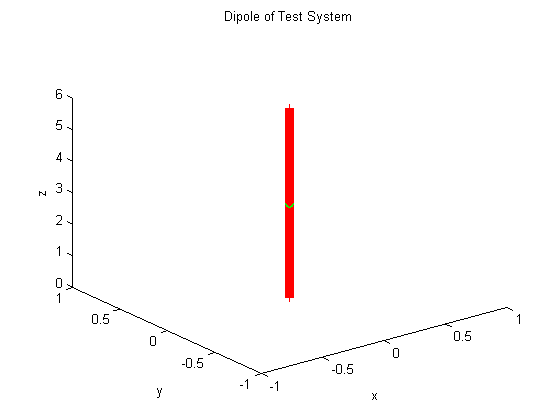
\includegraphics[width=12cm]{DissPics/dipol}\\
  \caption{6 meter dipole used for calculation}\label{figDipol}
\end{figure}

\section{A dipole in isotropic cold plasma}
\subsection{Computing the electric field pattern}
As a first step, an algorithm as described in Appendix B and shown in Appendix C was constructed and used to compute the electric field patterns of a dipole at various relations of antenna length to wavelength. The algorithm is valid for vacuum and isotropic plasmas, but the current distribution of the vacuum calculation is used at this stage. Several configurations in vacuum were computed and compared with results of proved programs for validation. These configurations will be used to investigate the effect of the different plasma models on the radiation pattern. The radiation patterns of the electric field strength are shown on Figures \ref{figNFvac10m300kHz} - \ref{figNFvac10m3halbelambdaMHz}. \\

A second solver was implemented, using sinusoidal base functions, for comparison. This solver, being much faster, produced the same results. The algorithm and source code of this solver is not presented in the thesis.\\

\begin{figure}
\begin{center}
  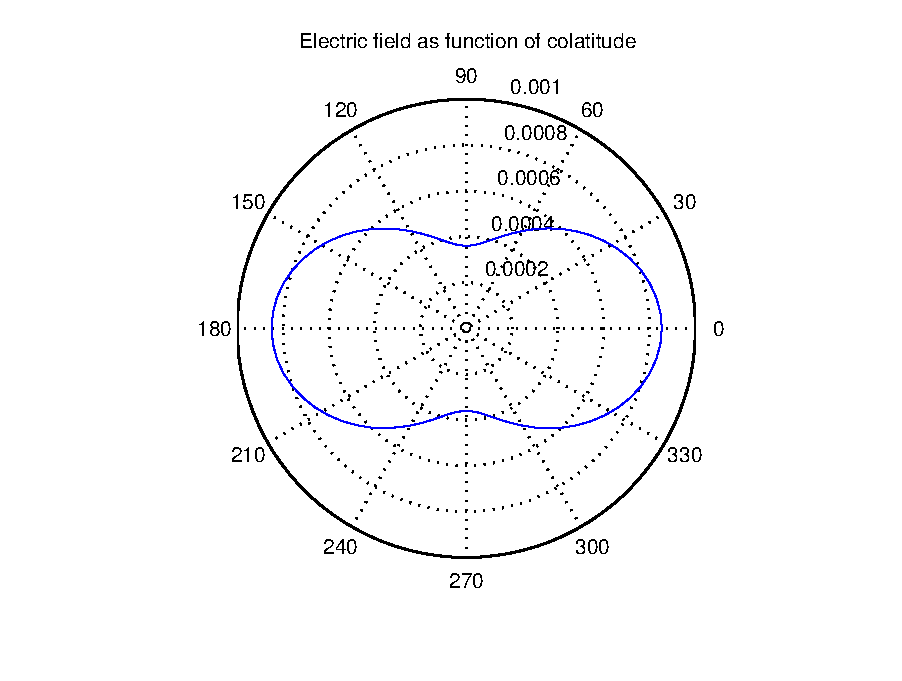
\includegraphics[width=11.5cm]{DissPics/NFvac10m300kHz.eps}
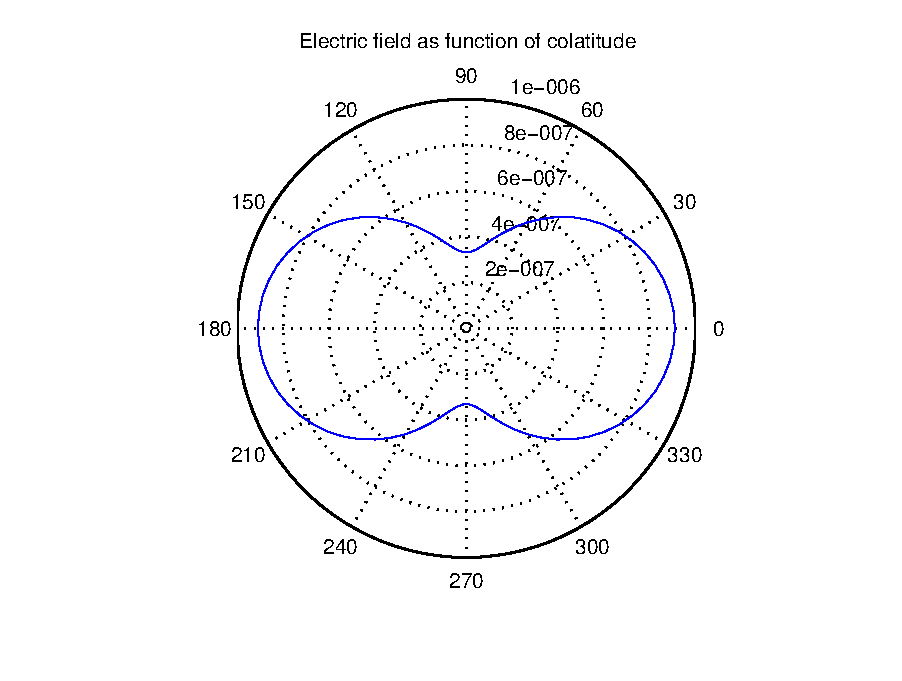
\includegraphics[width=11.5cm]{DissPics/NFvac100m300kHz.eps}
  \caption{Electric field strength $[Vm^{-1}]$ at 10m (top) and 100m (bottom) distance in at 300kHz}\label{figNFvac10m300kHz}
  \end{center}
\end{figure}

\begin{figure}
\begin{center}
  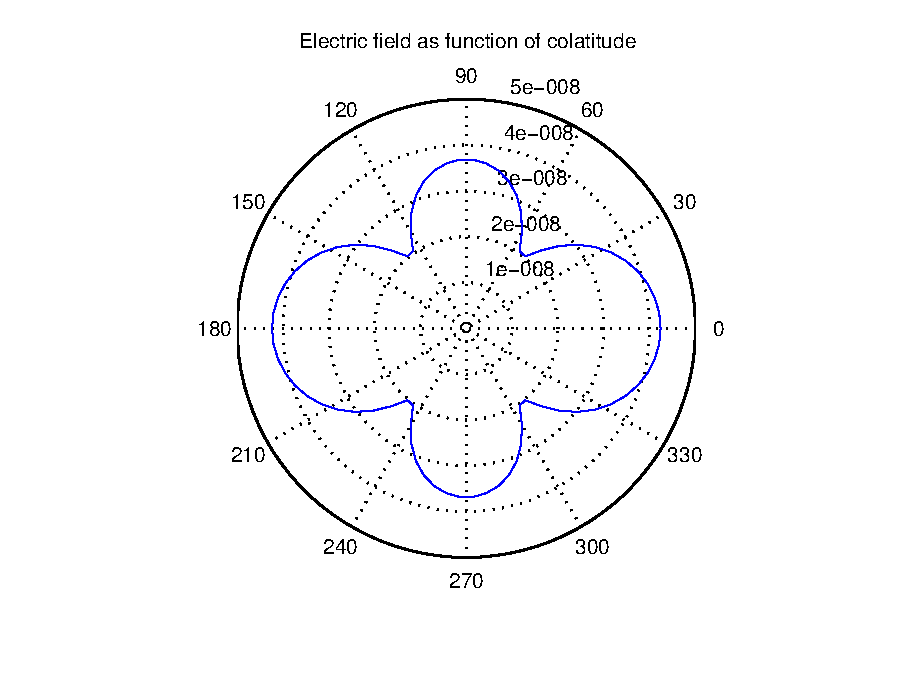
\includegraphics[width=11.5cm]{DissPics/NFvac300m300kHz.eps}
 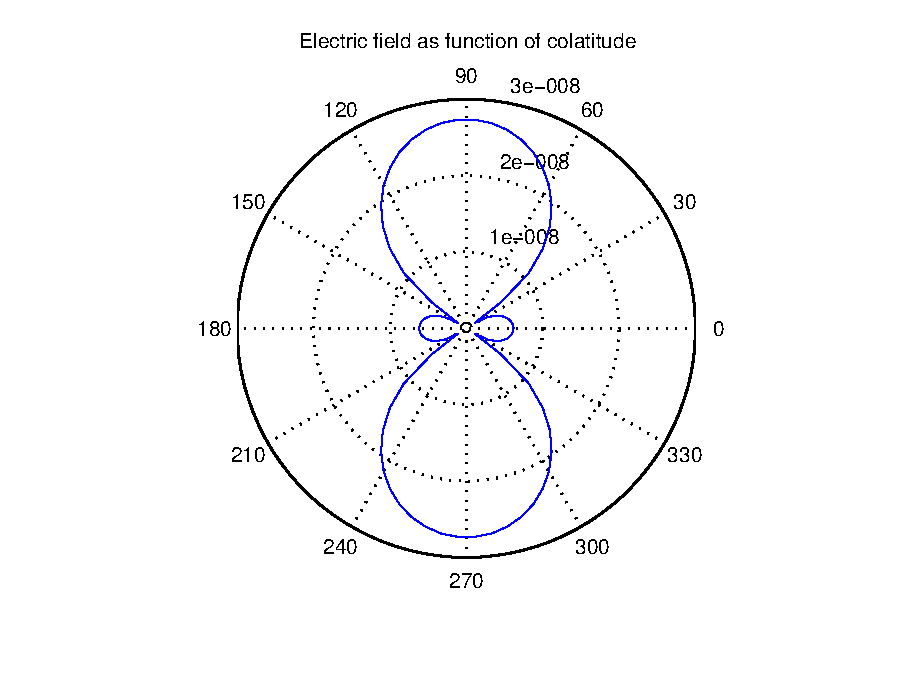
\includegraphics[width=11.5cm]{DissPics/NFvac500m300kHz.eps}
  \caption{Electric field strength $[Vm^{-1}]$ at 300m (top) and 500m (bottom) distance in vacuum at 300kHz}\label{figNFvac300m300kHz}
  \end{center}
\end{figure}


\begin{figure}
\begin{center}
  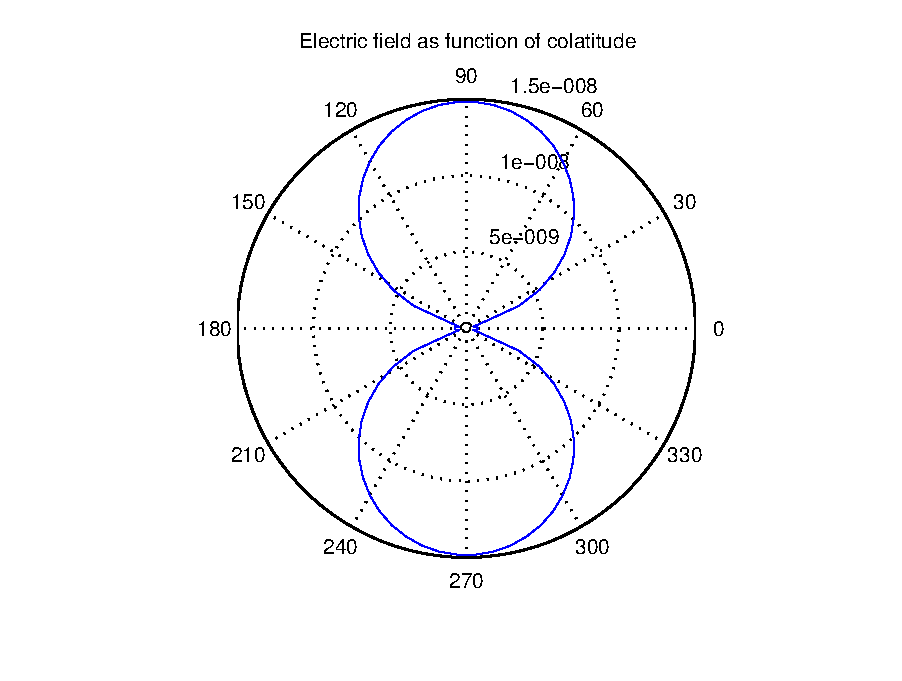
\includegraphics[width=11.5cm]{DissPics/NFvac1000m300kHz.eps}
 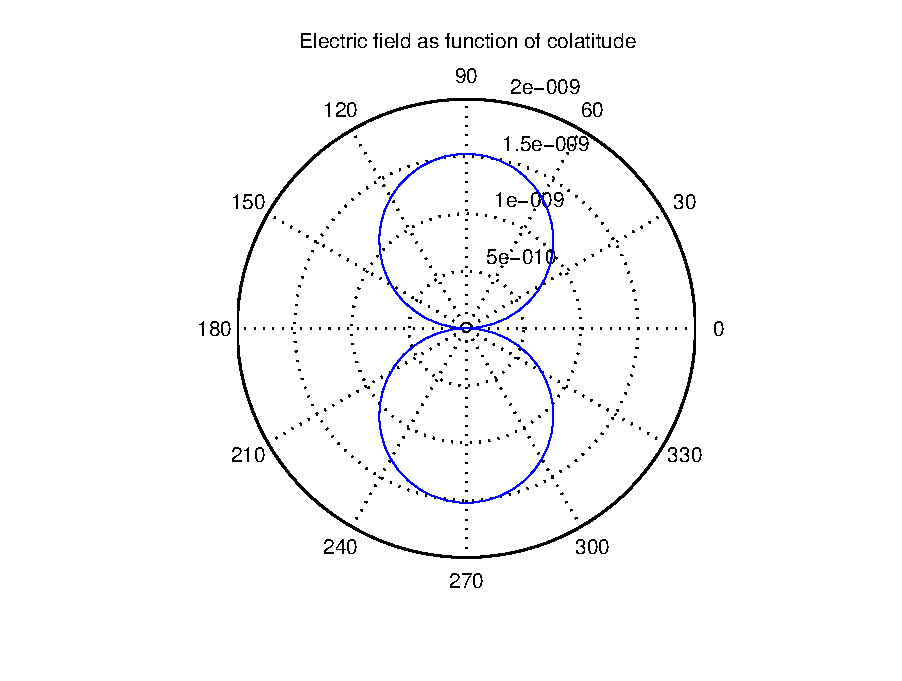
\includegraphics[width=11.5cm]{DissPics/NFvac10000m300kHz.eps}
  \caption{Electric field strength $[Vm^{-1}]$ at 1000m (top) and 10000m (bottom) distance in vacuum at 300kHz}\label{figNFvac1000m300kHz}
  \end{center}
\end{figure}

\begin{figure}
\begin{center}
  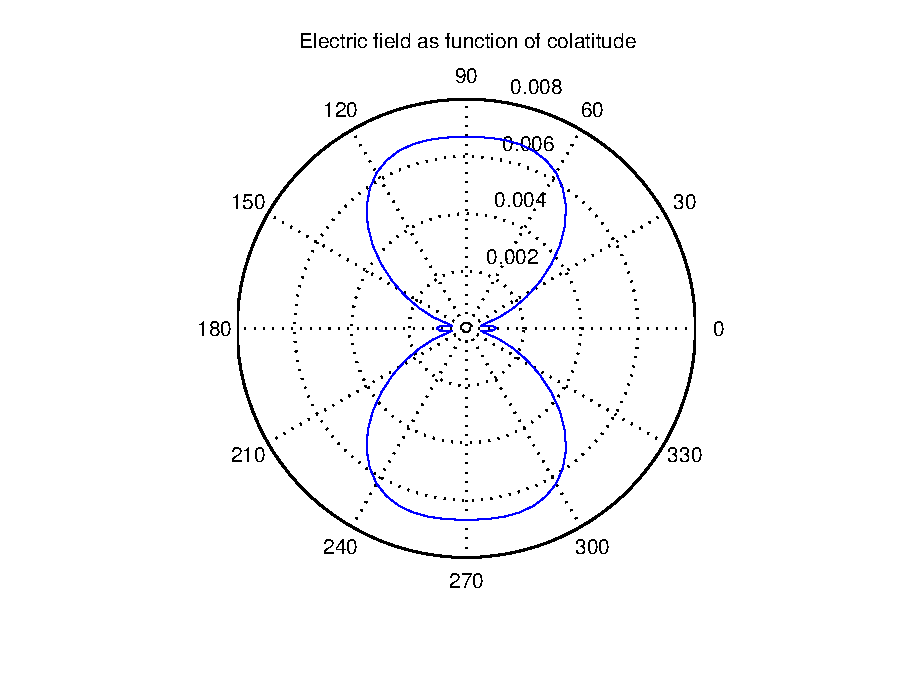
\includegraphics[width=11.5cm]{DissPics/NFvac10m50MHz.eps}
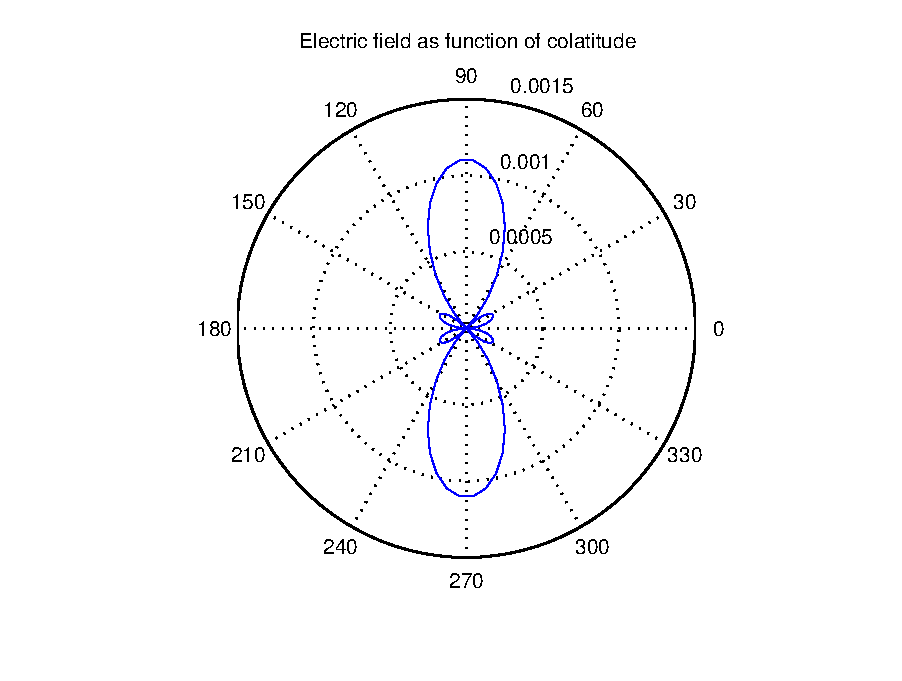
\includegraphics[width=11.5cm]{DissPics/NFvac50m50MHz.eps}
  \caption{Electric field strength $[Vm^{-1}]$ at 10m (top) and 50m (bottom) distance in vacuum at 50MHz}\label{figNFvac10m50MHz}
  \end{center}
\end{figure}


\begin{figure}
\begin{center}
  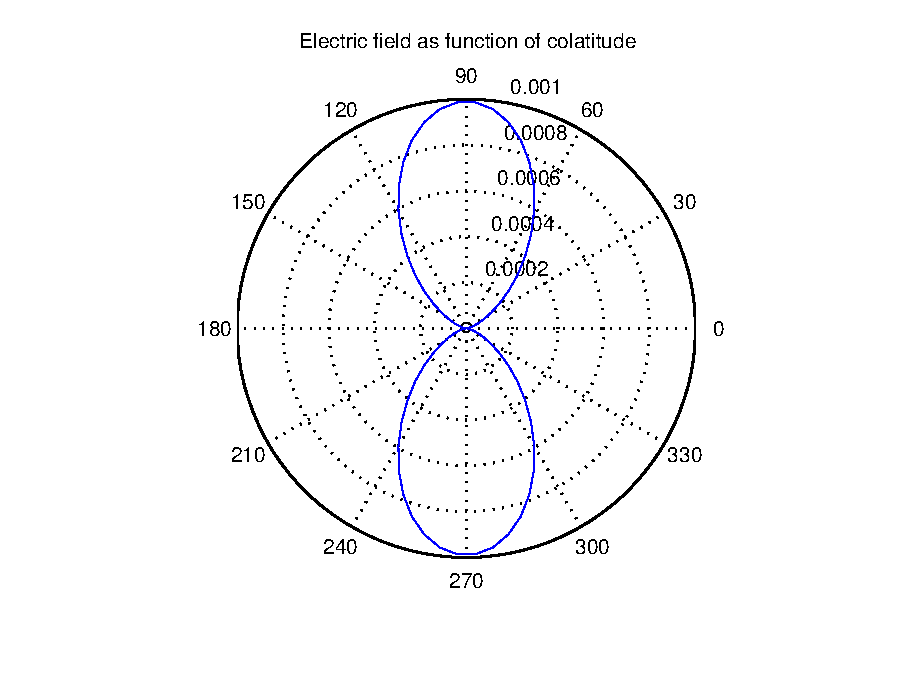
\includegraphics[width=11.5cm]{DissPics/NFvac100m50MHz.eps}
 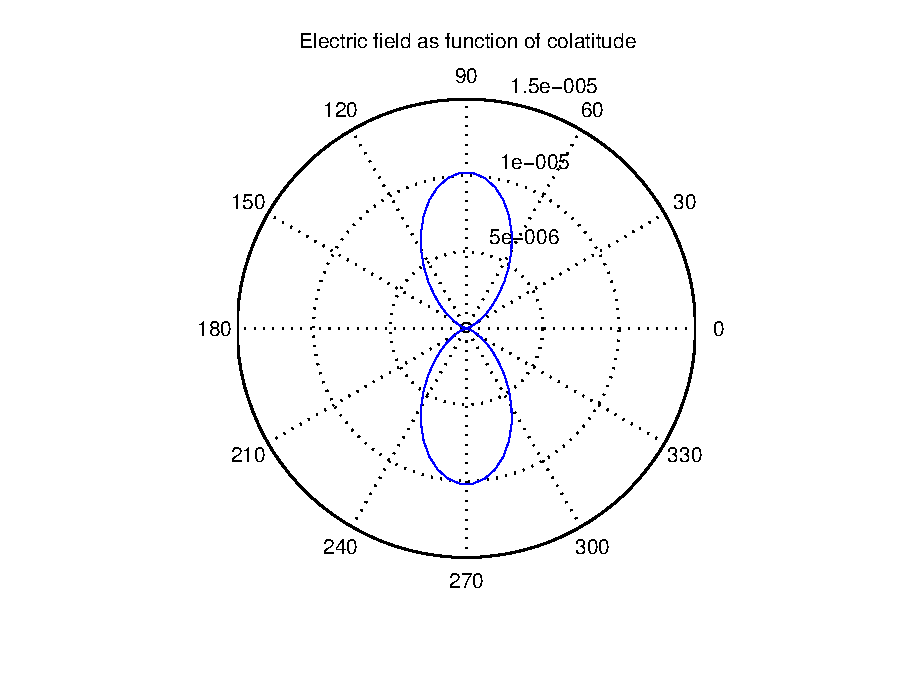
\includegraphics[width=11.5cm]{DissPics/NFvac10000m50MHz.eps}
  \caption{Electric field strength $[Vm^{-1}]$ at 100m (top) and 10000m (bottom) distance in vacuum at 50MHz}\label{figNFvac100m50MHz}
  \end{center}
\end{figure}


\begin{figure}
\begin{center}
  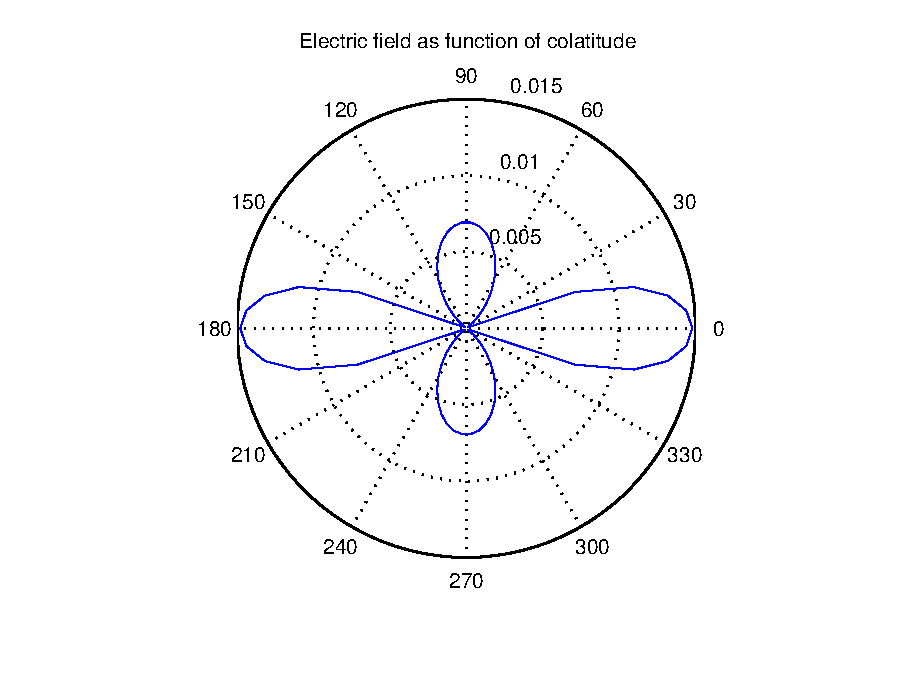
\includegraphics[width=11.5cm]{DissPics/NFvac10m25MHz.eps}
 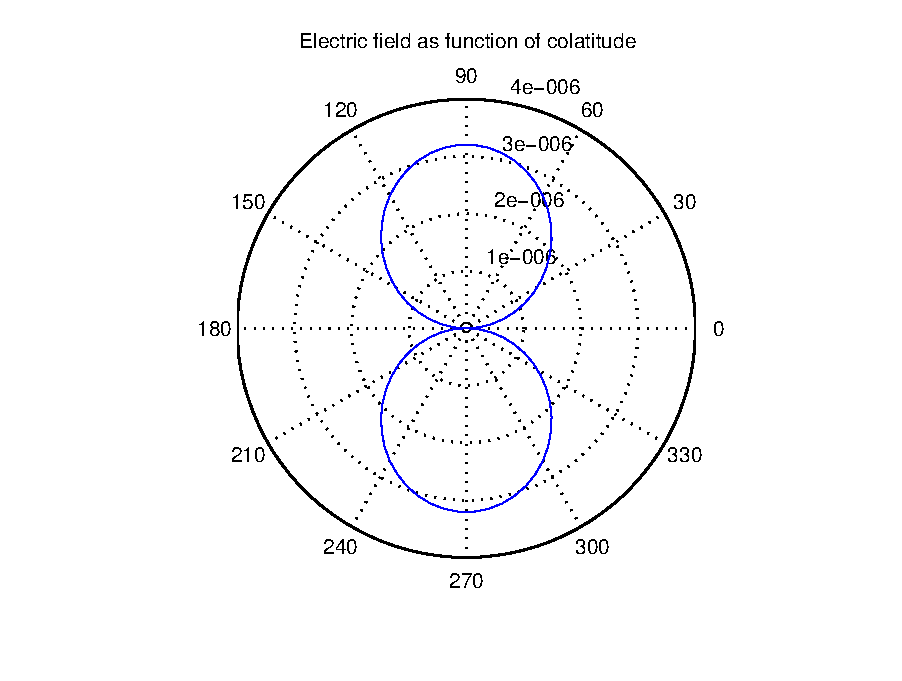
\includegraphics[width=11.5cm]{DissPics/NFvac10000m25MHz.eps}
  \caption{Electric field strength $[Vm^{-1}]$ at 10m (top) and 10000m (bottom) distance in vacuum at 25MHz}\label{figNFvac10m25MHz}
  \end{center}
\end{figure}



\begin{figure}
\begin{center}
  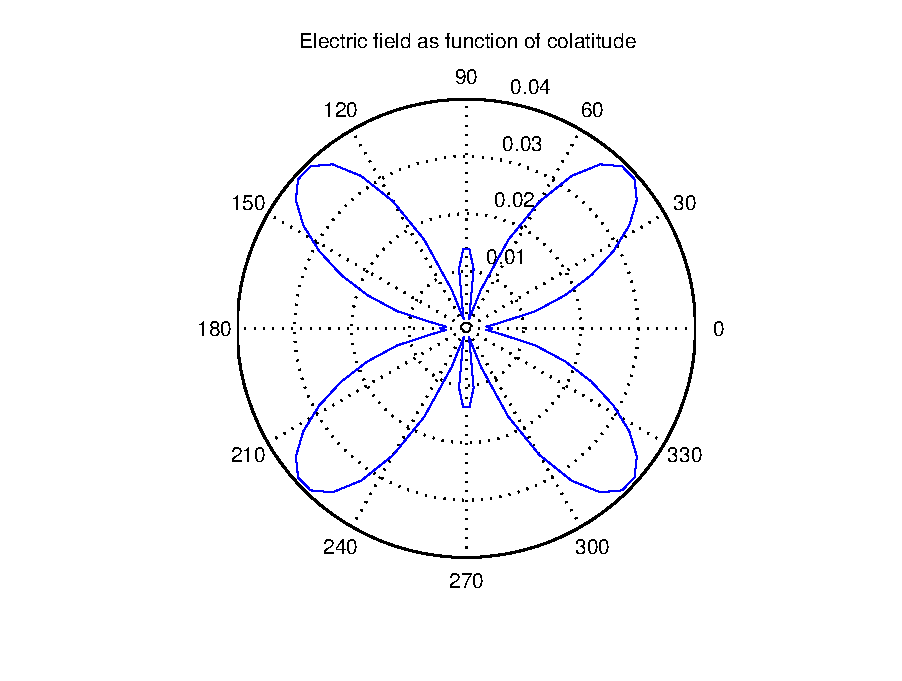
\includegraphics[width=11.5cm]{DissPics/NFvac10m3halbelambdaMHz.eps}
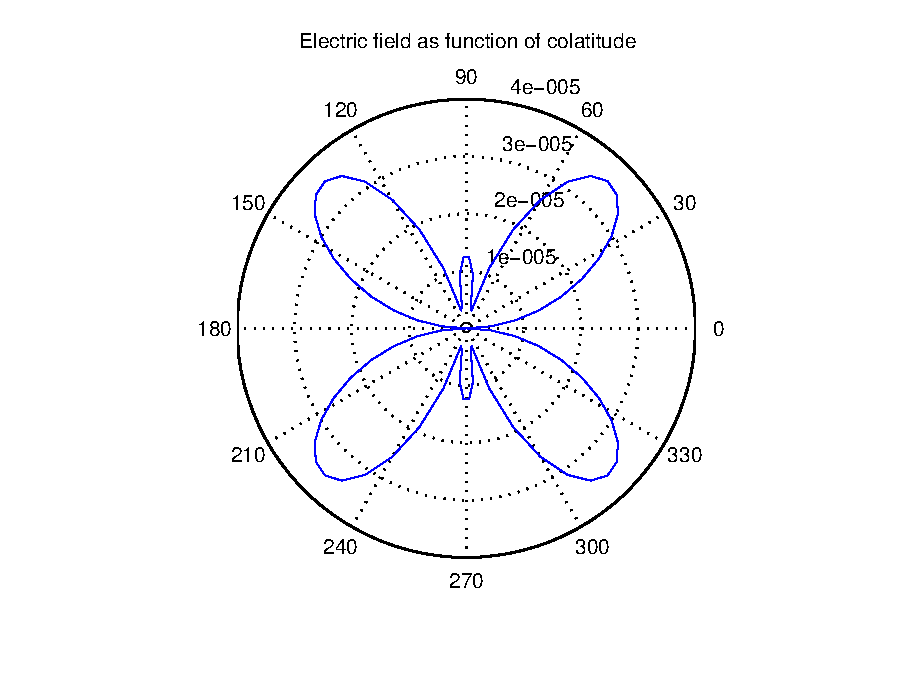
\includegraphics[width=11.5cm]{DissPics/NFvac10000m3halbelambdaMHz.eps}
  \caption{Electric field strength $[Vm^{-1}]$ at 10m (top) and 10000m (bottom) distance in vacuum at $\frac{3}{2}\lambda$ resonance condition}\label{figNFvac10m3halbelambdaMHz}
  \end{center}
\end{figure}


To compute the electric field for an isotropic cold plasma, the dielectric function (\ref{epsilon_plasma}) can be used. At the first run the so-called radio approximation is used, which ignores the influence of the ions. The determining factor of the E-field pattern is the squared relation between the frequency of the electromagnetic wave and the plasma frequency $\frac{\omega_{pe}^2}{\omega^2}$. Looking at eq. (\ref{isotropicelectricfield}), it can be noticed that the permittivity can be found in the denominator of the equation. Hence the effect of the permittivity on the electric field is of inverse proportional nature. There is a cutoff at the plasma frequency. At or below this cutoff frequency an ordinary propagation of electromagnetic waves is not possible. A second parameter, altered by the existence of the plasma which influences the magnitude of the electric field in this simple model, is the wave-number. Its influence outweighs the effect of the relative permittivity and therefore the magnitude of the electric field is expected to be smaller at a given point in space. The phase at a given distance from the antenna is also altered due to the wave-number in the exponent. Since the wave-number at a given frequency is smaller than in vacuum, the wave is elongated which results in a different near-field pattern at a given distance. At large distances the difference in shape vanishes and only the difference in magnitude of the field remains. So the far-field pattern can be expected to have the same shape, however a smaller magnitude.\\

Figure \ref{figNFisocold1000m300kHz0.9} shows a comparison between the radiation patterns at 10000m distance at 300kHz in vacuum and cold isotropic plasma with $\frac{\omega_{pe}^2}{\omega^2}=0.9$.\\

The physical reason for the decreasing effect of the plasma on the magnitude of the electric field is most likely, that in a steady state condition the plasma oscillates with the excitation frequency in the neighborhood of the antenna. Thus an additional form of energy is stored in each volume element. This energy is called ordered kinetic energy:

\begin{equation}
    E_{ok}=\sum_s \frac{1}{2} n_s m_s v_s^2
\end{equation}

$v_s$ is the drift speed of particle species s. The electric and magnetic energies have to be smaller by the amount of the ordered kinetic energy. The relation of magnetic and electric energy to the ordered kinetic energy is proportional to $\epsilon$. At the plasma frequency, the relation is equal to unity. Towards higher frequencies, the magnitude of the ordered kinetic energy becomes less in comparison to energy forms which exist also in vacuum. So the behavior of the antenna tends to the vacuum case when dealing with high frequencies.\\


\begin{figure}
\begin{center}
 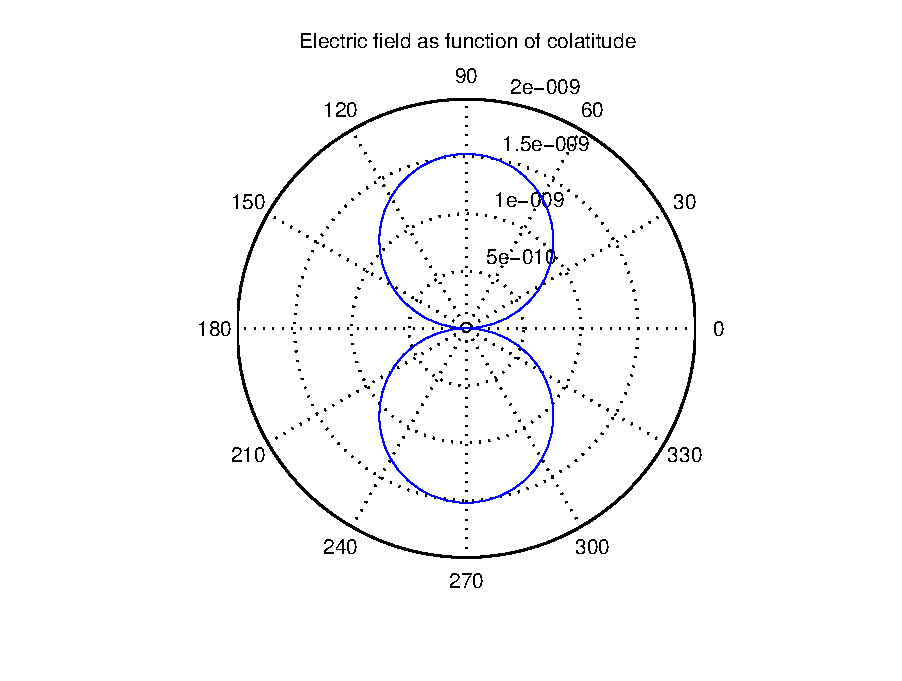
\includegraphics[width=11.5cm]{DissPics/NFvac10000m300kHz.eps}
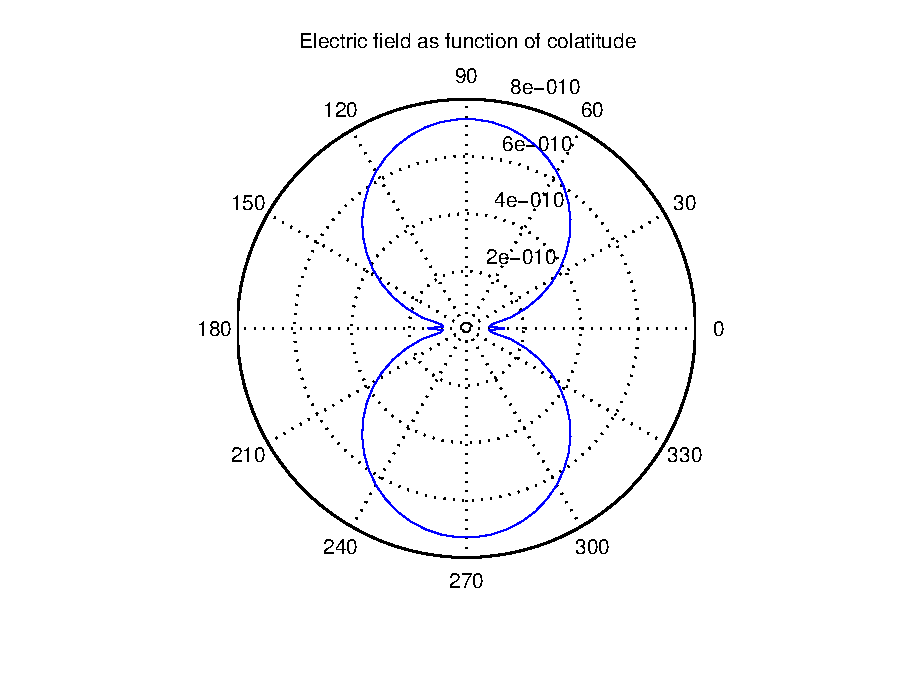
\includegraphics[width=11.5cm]{DissPics/NFisocold10000m300kHz0.9.eps}
  \caption{Electric field strength $[Vm^{-1}]$ at 10000m distance in vacuum (top) and isotropic cold plasma (bottom) with $\frac{\omega_{pe}^2}{\omega^2}=0.9$ at 300kHz}\label{figNFisocold1000m300kHz0.9}
\end{center}
\end{figure}


Taking the effect of the ions into account results in Figure \ref{figNFisocoldwithions1000m300kHz0.9}. The difference to the radio approximation is small but noticeable. The effect of the ions is less then the effect of the electrons by roughly a factor of 2000, which is the mass ratio between ion and electron. So the ratio of the plasma frequencies is $\sqrt{2000}$ and therefore $\frac{\omega_{pi}^2}{\omega_{pe}^2}\approx \frac{1}{2000}$. This result is only true for hydrogen ions when the ion density is equal to the electron density, because these 2 parameters are also part of the formulas of the plasma frequencies and therefore influence the radiated field.

\begin{figure}
\begin{center}
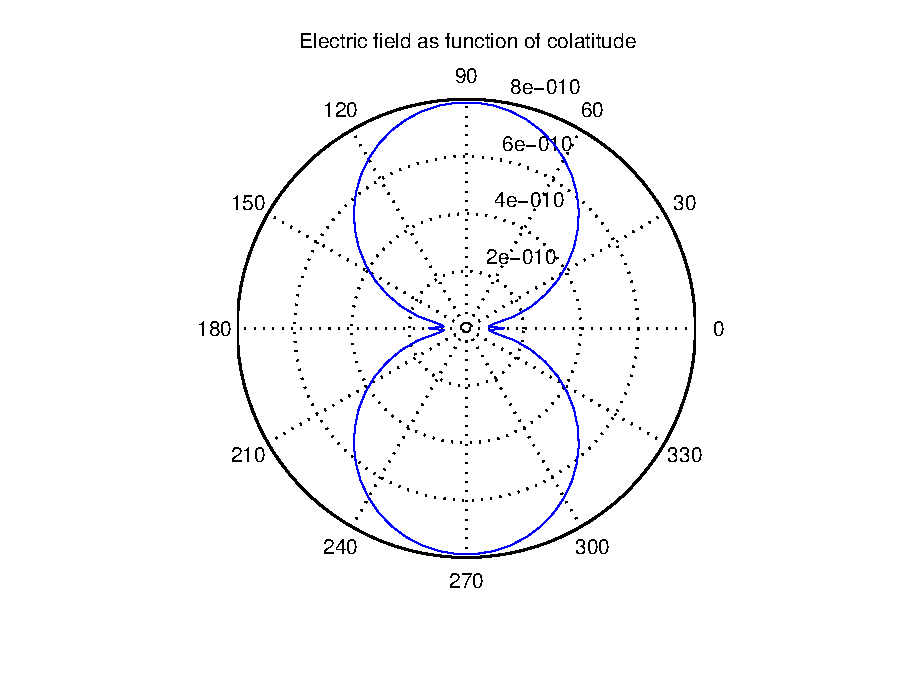
\includegraphics[width=11.5cm]{DissPics/NFisocoldwithions10000m300kHz0.9.eps}
  \caption{Electric field strength $[Vm^{-1}]$ 10000m distance in isotropic cold plasma with $\frac{\omega_{pe}^2}{\omega^2}=0.9$, taking the effect of ions into account, at 300kHz}\label{figNFisocoldwithions1000m300kHz0.9}
\end{center}
\end{figure}

Figure \ref{fig:NFisocold_twommore} shows two examples with other input parameters to demonstrate the change in shape of the pattern.

\begin{figure}
\begin{center}
 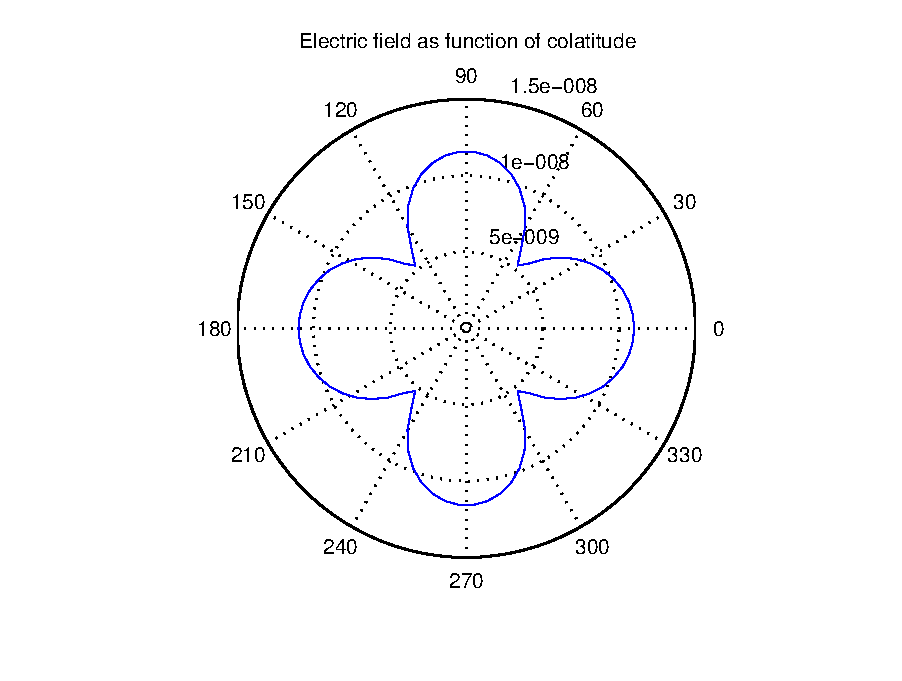
\includegraphics[width=11.5cm]{DissPics/NFisocoldwithions1000m300kHz0.9.eps}
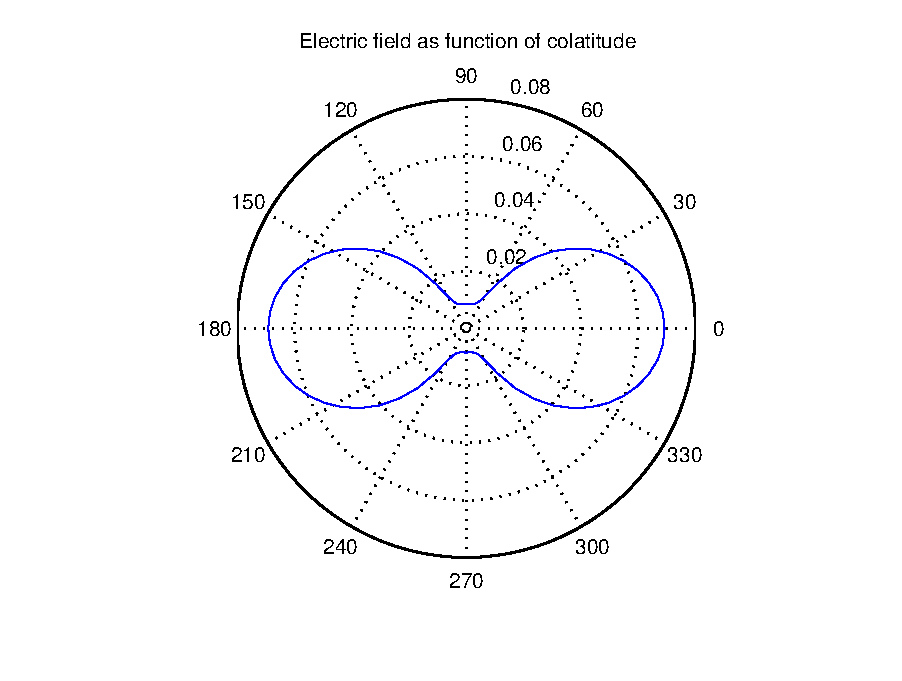
\includegraphics[width=11.5cm]{DissPics/NFisocoldwithions10m25MHz0.9.eps}   \caption{Electric field strength $[Vm^{-1}]$ 1000m distance isotropic cold plasma with $\frac{\omega_{pe}^2}{\omega^2}=0.9$ at 300kHz (top), as well as in 10m at 25MHz (bottom)}\label{fig:NFisocold_twommore}
\end{center}
\end{figure}

\subsection{The effect of plasma on the current distribution}
The next logical step is to investigate the influence of the plasma on the current distribution. A very simple fortran program was written to implement the Method of Moments (MoM) as described in \cite{kraus}. The parameters which are modified by the plasma in this model are the impedance of free space and the wavelength. Since the modifications are inside as well as outside the exponent, the current is expected to change in magnitude and shape. Due to the change of shape the resonance frequency is expected to be shifted and the antenna input impedance, which is the relation of the voltage at the feed to the current at the feed is expected to change. The calculations has been performed for several frequencies using the test dipole of 6 meters length. The effect of the ions has been included in the computation and the relation between the squares of the frequency and the electron plasma frequency is 0.9.\\

Figures \ref{fig:curr_3kh_vac} and \ref{fig:curr_3kh_pl} show the current distributions at 300 kilohertz in vacuum and cold isotropic plasma, respectively. At this wavelength which is much longer than the antenna, the difference in shape is not noticeable. One can see the difference in magnitude though. The calculated input impedances are $6.5065 \cdot 10^{-3} -3.5590\cdot 10^4\imath$ ohms and $2.0527\cdot 10^{-3} -3.575\cdot 10^5\imath$ ohms to 5 significant figures. So a clear difference is noticeable.\\

\begin{figure}
 \begin{center}
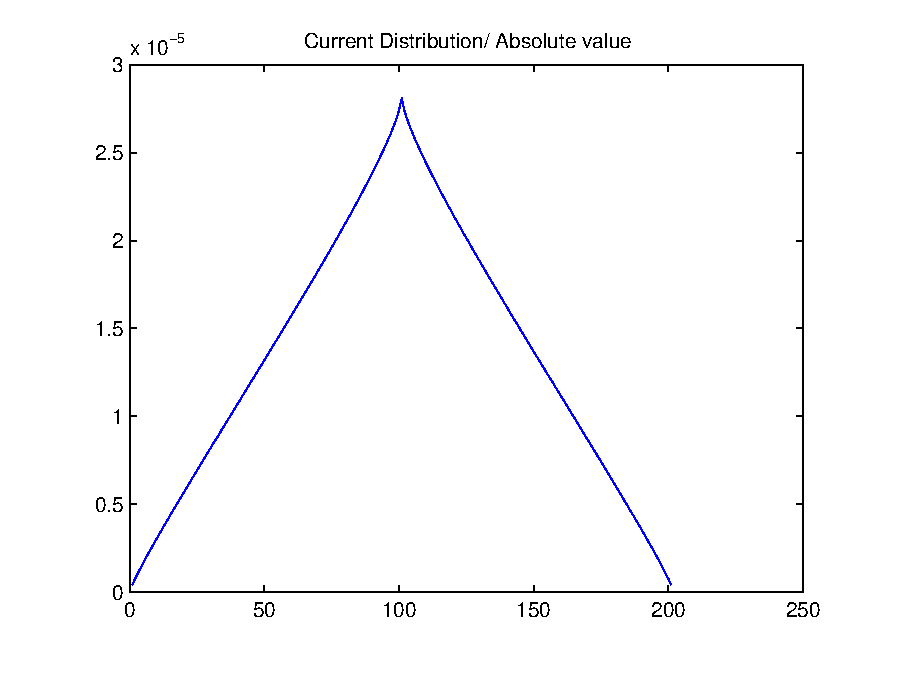
\includegraphics[width=10.0cm]{DissPics/curr_abs_3kh.eps}
 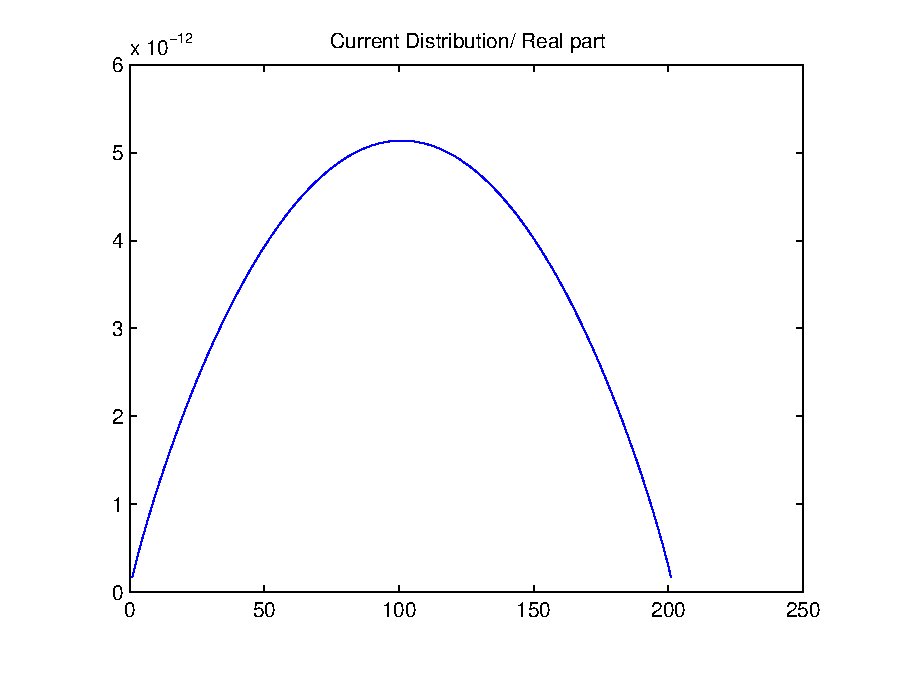
\includegraphics[width=10.0cm]{DissPics/curr_re_3kh.eps}
 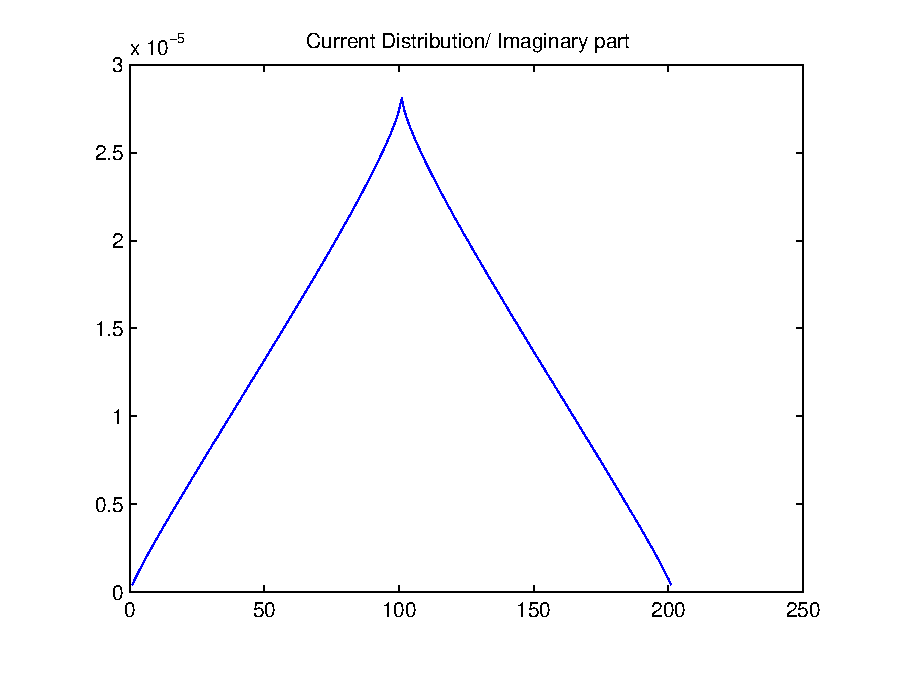
\includegraphics[width=10.0cm]{DissPics/curr_im_3kh.eps}\end{center}
  \caption{The current distribution [A] (y-axis) along the dipole segments (x-axis) at 300kHz in vacuum}\label{fig:curr_3kh_vac}
\end{figure}

\begin{figure}
 \begin{center}
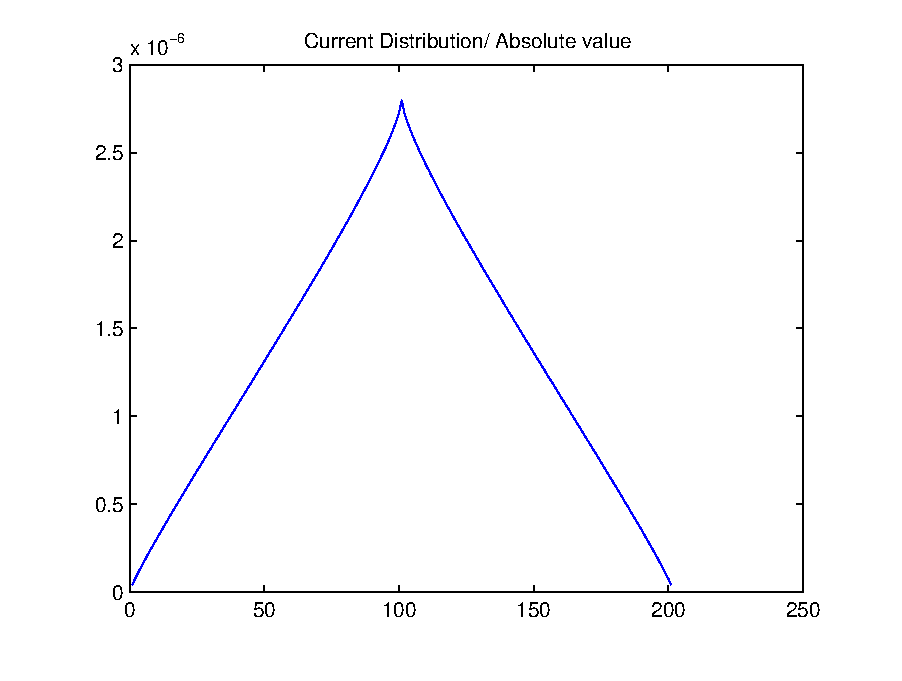
\includegraphics[width=10.0cm]{DissPics/curr_abs_3kh_p.eps}
 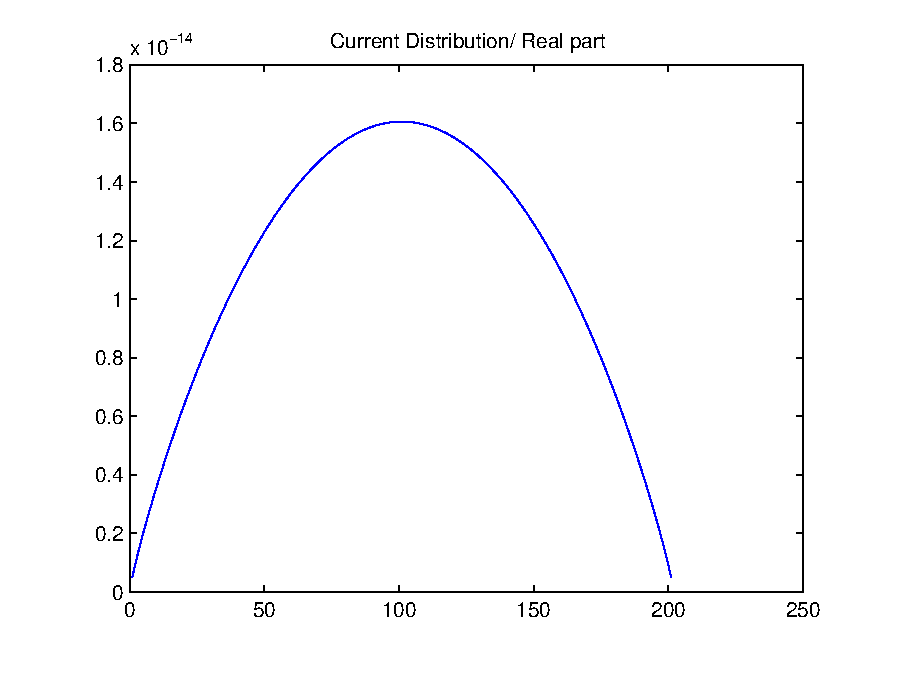
\includegraphics[width=10.0cm]{DissPics/curr_re_3kh_p.eps}
 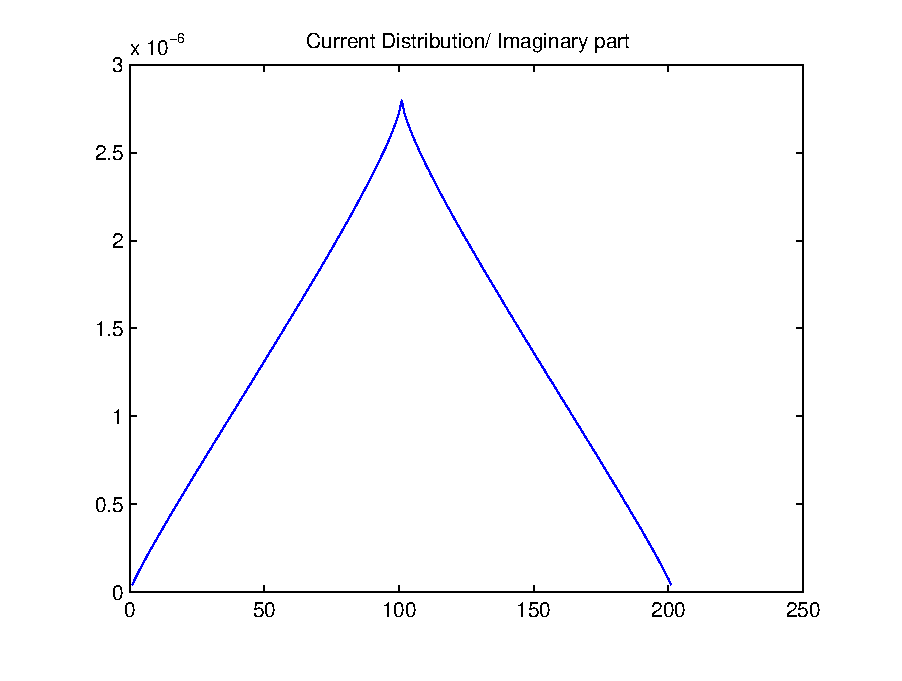
\includegraphics[width=10.0cm]{DissPics/curr_im_3kh_p.eps}\end{center}
  \caption{The current distribution [A] (y-axis) along the dipole segments (x-axis) at 300kHz in plasma}\label{fig:curr_3kh_pl}
\end{figure}

Figures \ref{fig:curr_3mh_vac} to \ref{fig:curr_30mh_pl} show the respective results of calculations with 3MHz and 30MHz. Here the change of shape is more pronounced. The increase of wavelength can be seen. The calculated input impedances are $1.919\cdot 10^2 +4.1009\cdot10^2\imath$ ohms, $2.231 -3.0747\cdot10^3\imath$ ohms, $9.5611 -2.403\cdot 10^2\imath$ ohms, and
$3.137\cdot 10^3 -3.296\cdot 10^3\imath$ ohms.\\

\begin{figure}
 \begin{center}
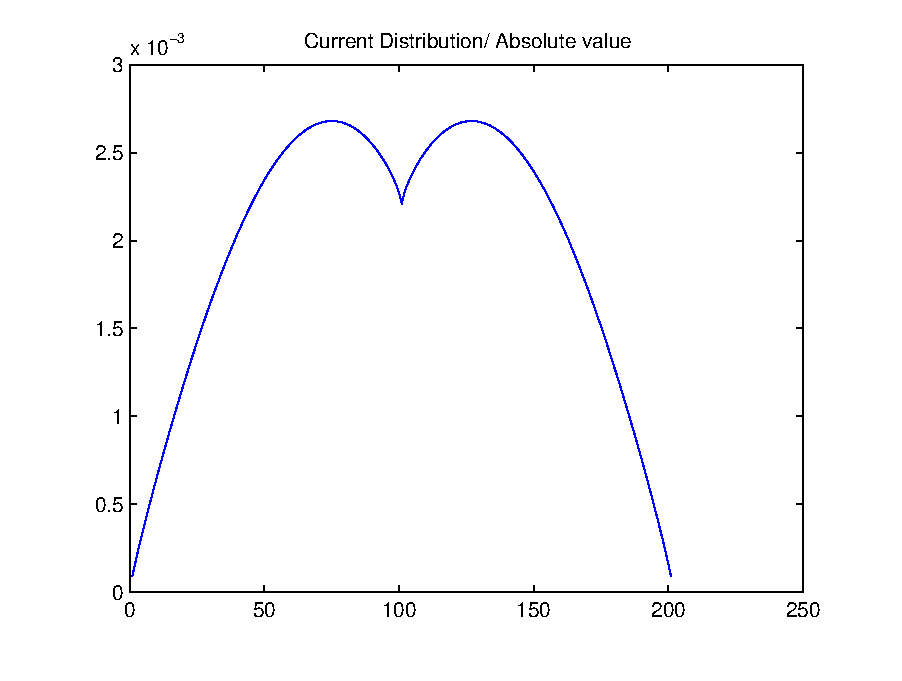
\includegraphics[width=10.0cm]{DissPics/curr_abs_3mh.eps}
 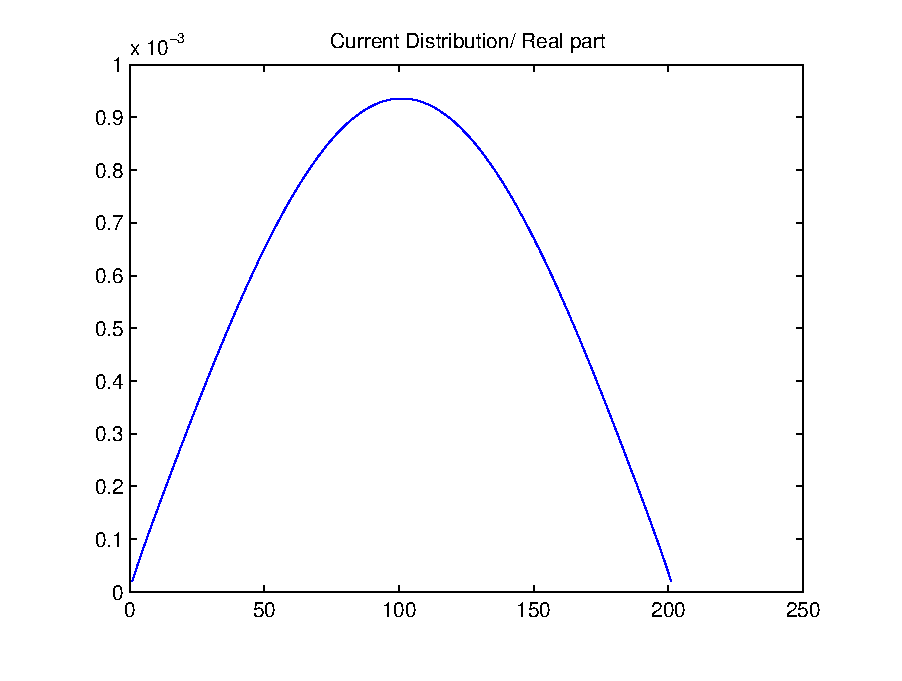
\includegraphics[width=10.0cm]{DissPics/curr_re_3mh.eps}
 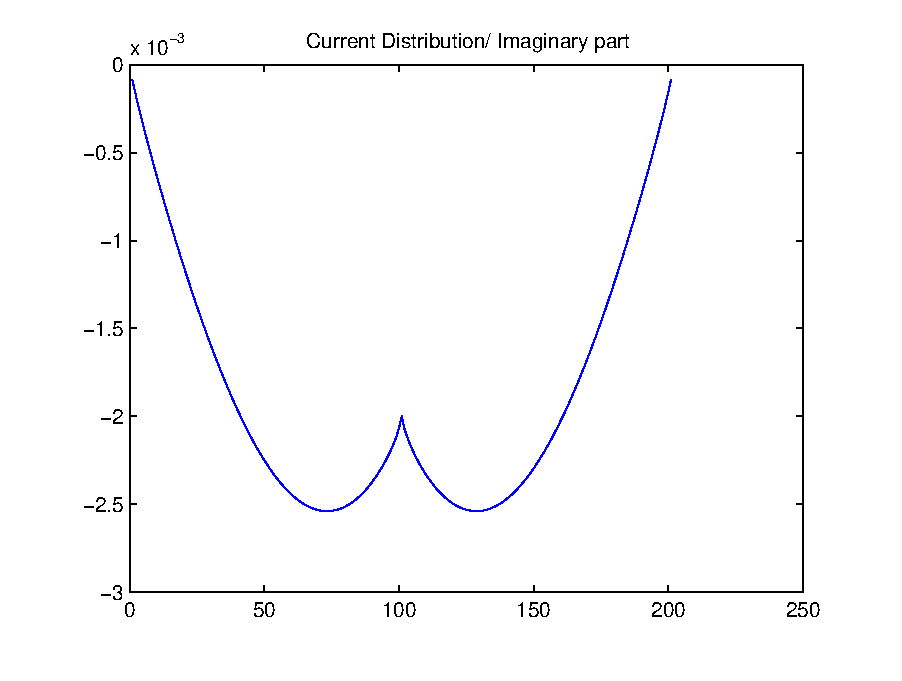
\includegraphics[width=10.0cm]{DissPics/curr_im_3mh.eps}\end{center}
  \caption{The current distribution [A] (y-axis) along the dipole segments (x-axis) at 3MHz in vacuum}\label{fig:curr_3mh_vac}
\end{figure}

\begin{figure}
 \begin{center}
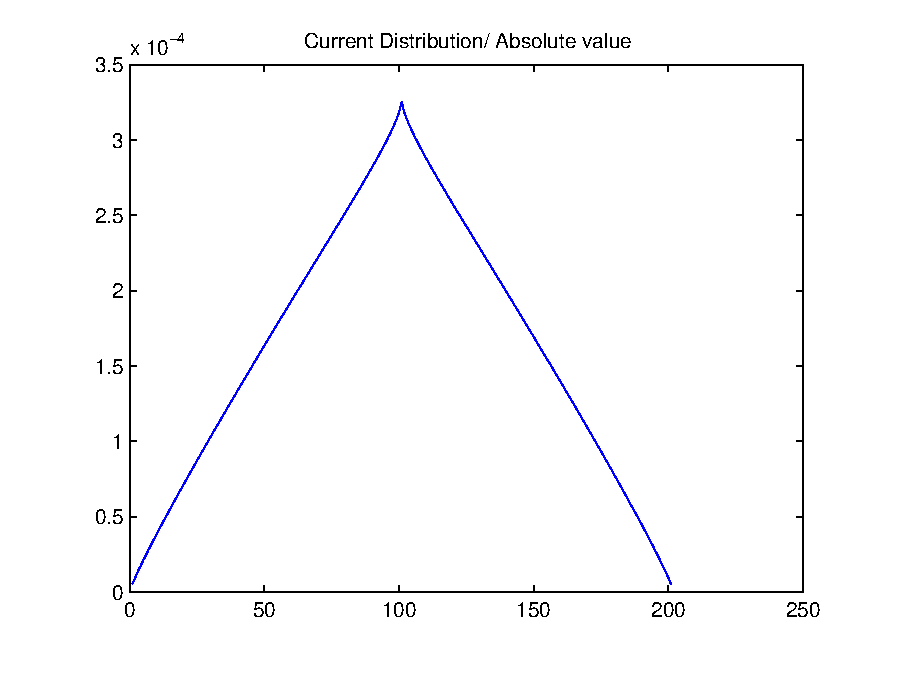
\includegraphics[width=10.0cm]{DissPics/curr_abs_3mh_p.eps}
 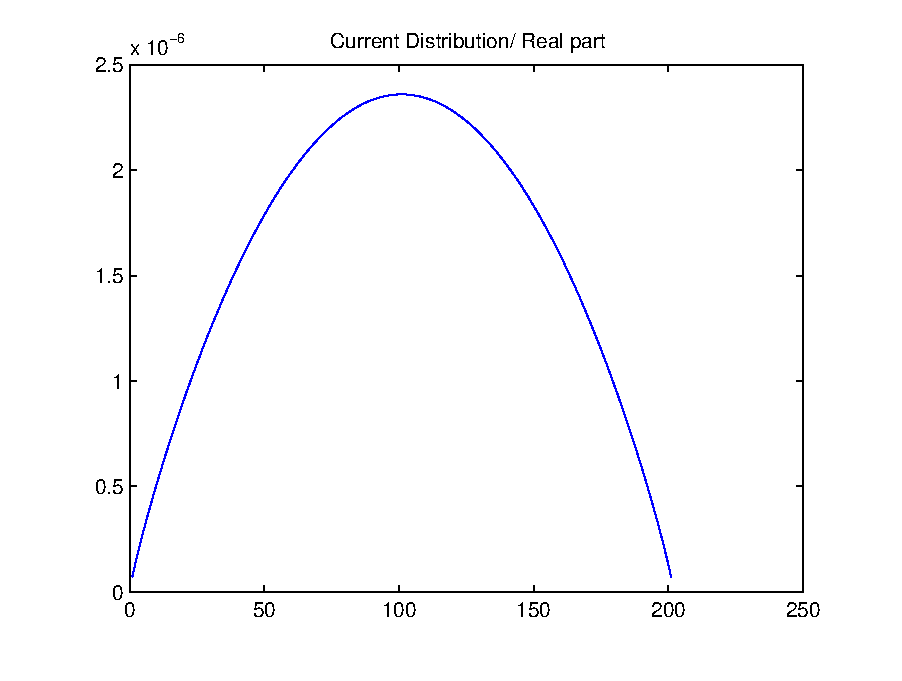
\includegraphics[width=10.0cm]{DissPics/curr_re_3mh_p.eps}
 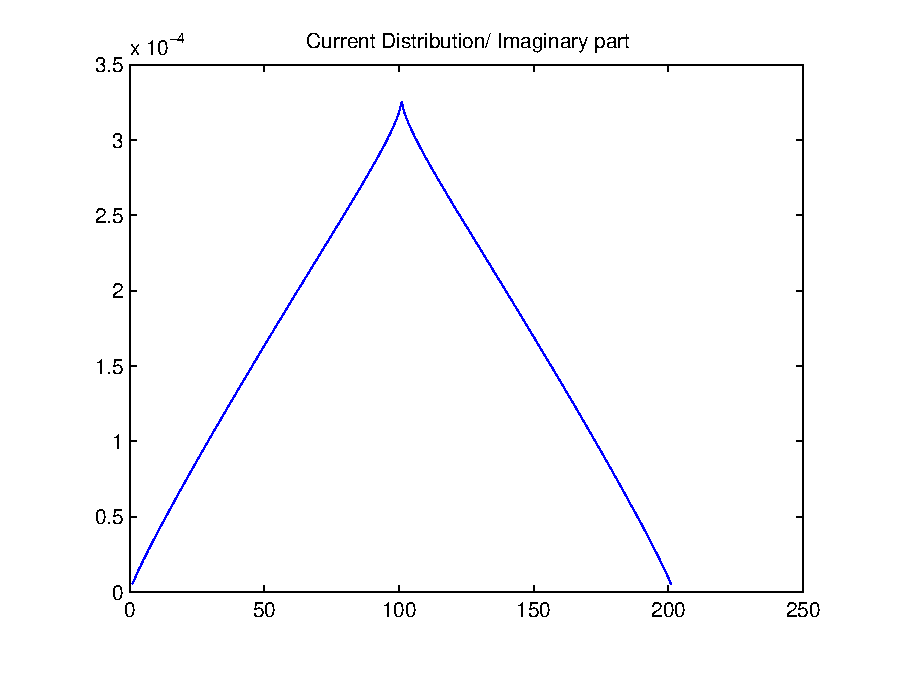
\includegraphics[width=10.0cm]{DissPics/curr_im_3mh_p.eps}\end{center}
  \caption{The current distribution [A] (y-axis) along the dipole segments (x-axis) at 3MHz in plasma}\label{fig:curr_3mh_pl}
\end{figure}

\begin{figure}
 \begin{center}
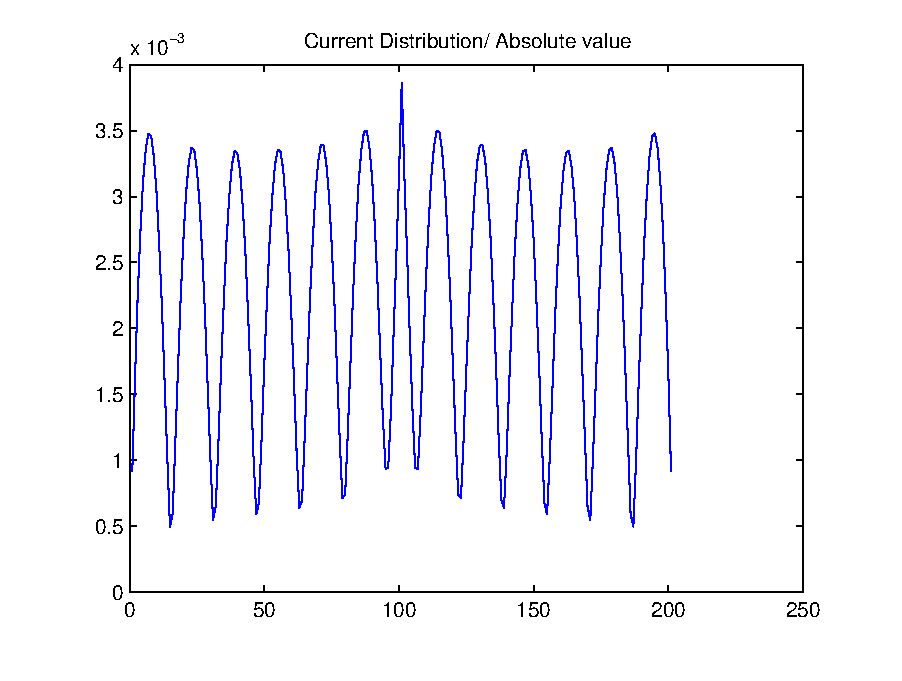
\includegraphics[width=10.0cm]{DissPics/curr_abs_30mh.eps}
 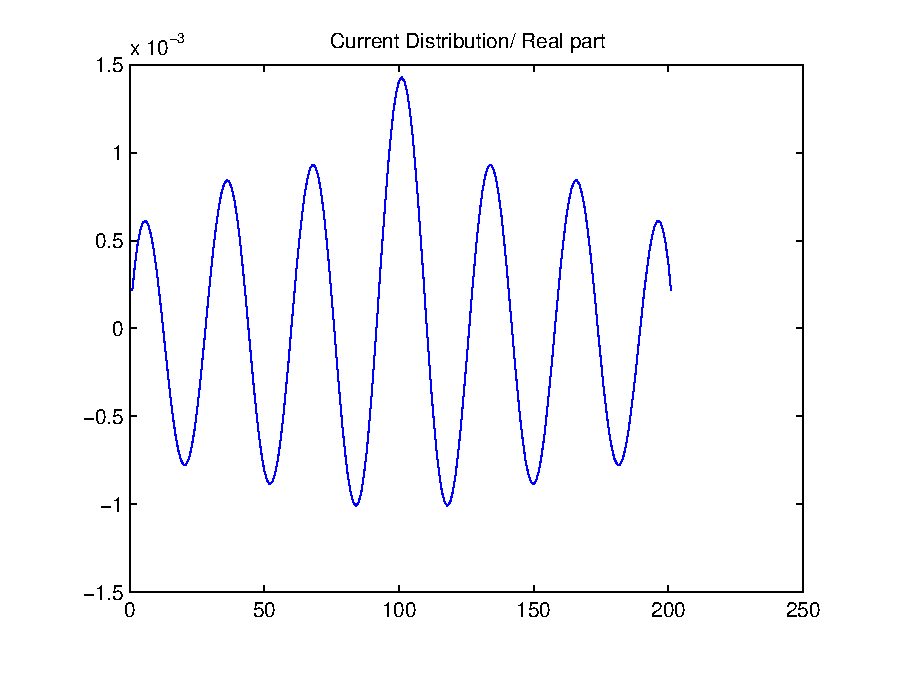
\includegraphics[width=10.0cm]{DissPics/curr_re_30mh.eps}
 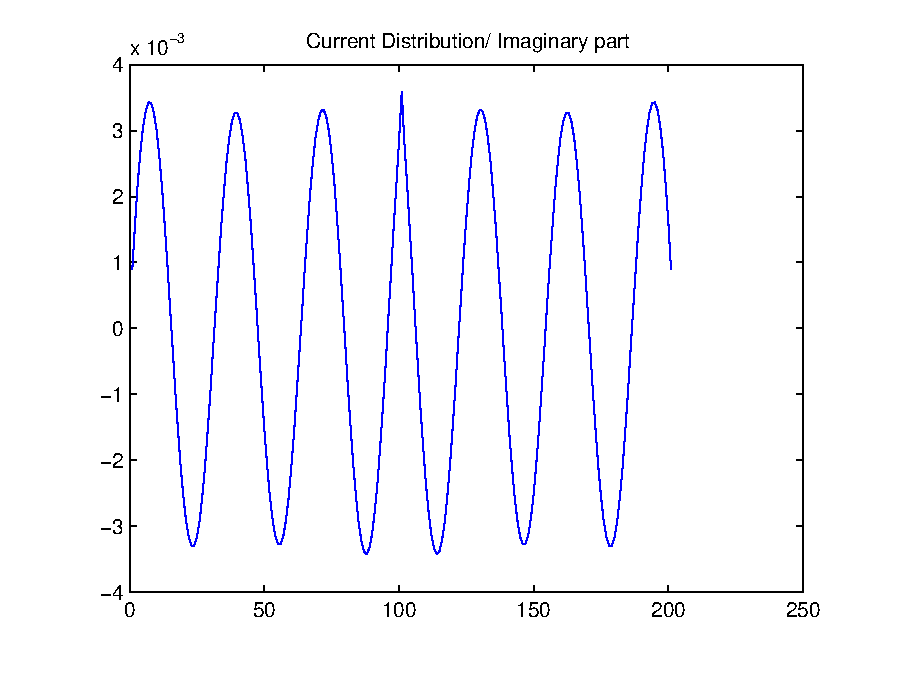
\includegraphics[width=10.0cm]{DissPics/curr_im_30mh.eps}\end{center}
  \caption{The current distribution [A] (y-axis) along the dipole segments (x-axis) at 30MHz in vacuum}\label{fig:curr_30mh_vac}
\end{figure}

\begin{figure}
 \begin{center}
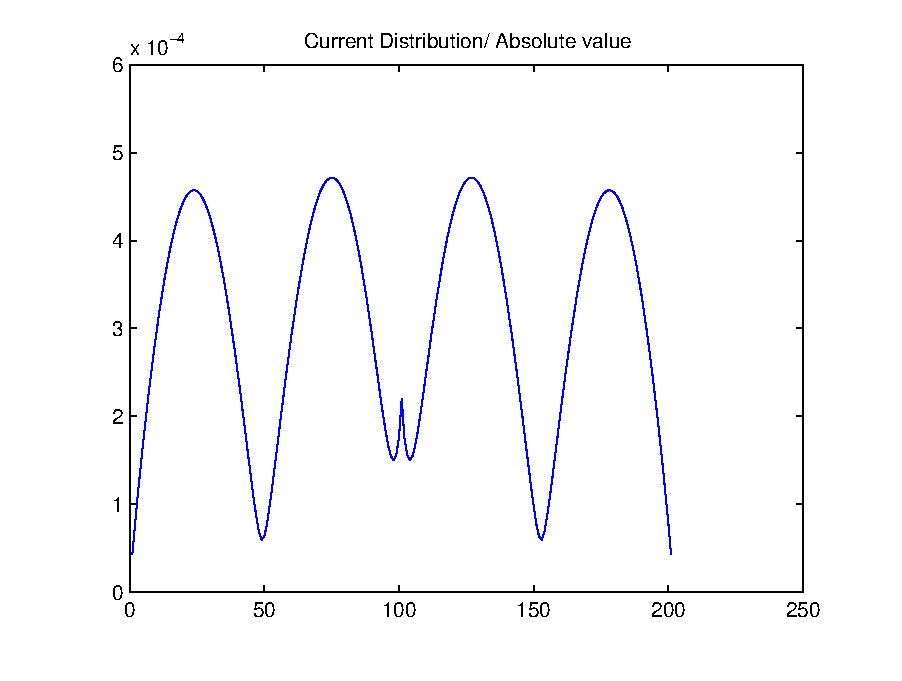
\includegraphics[width=10.0cm]{DissPics/curr_abs_30mh_p.eps}
 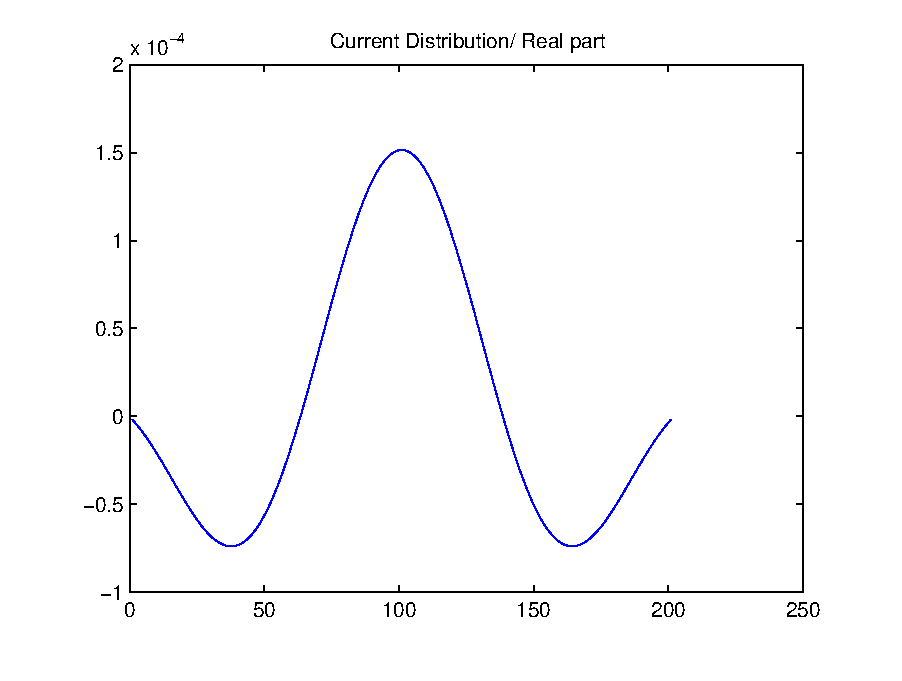
\includegraphics[width=10.0cm]{DissPics/curr_re_30mh_p.eps}
 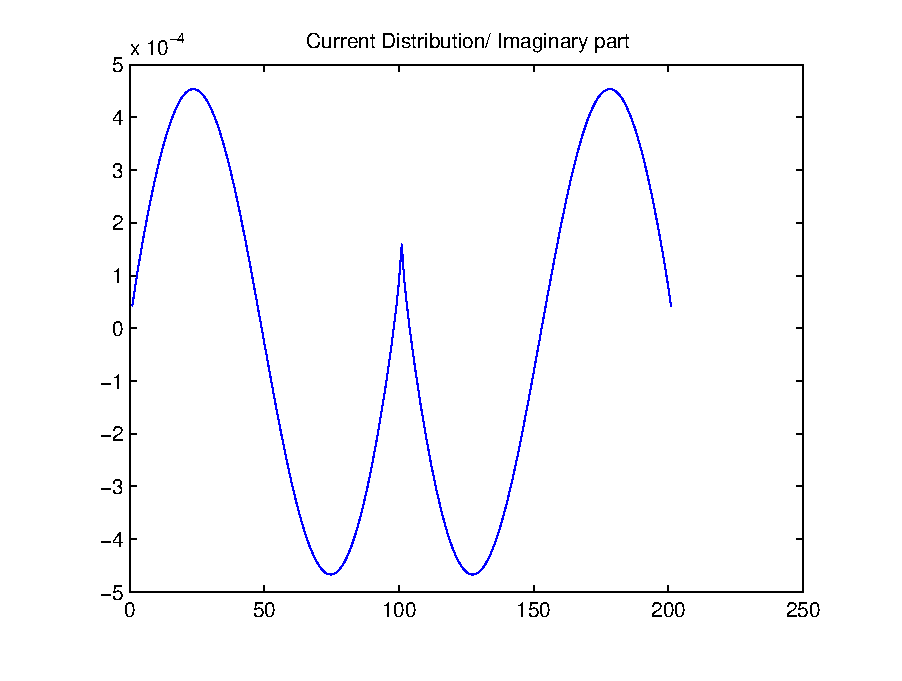
\includegraphics[width=10.0cm]{DissPics/curr_im_30mh_p.eps}\end{center}
  \caption{The current distribution [A] (y-axis) along the dipole segments (x-axis) at 30MHz in plasma}\label{fig:curr_30mh_pl}
\end{figure}

Figure \ref{fig:imps_fixed} shows the real and imaginary part of the input impedance as a function of frequency. The relation between squared frequency and plasma frequency of the electrons is $0.9$ in the whole range. This is not a realistic scenario, but good for demonstration how a high electron content modifies the impedance at a given frequency. The first resonances can be seen in the curve of the impedance in vacuum. The curve of the impedance in plasma shows only the first resonance, i.e. the point where the curve crosses the x-axis. This is the expected behavior.\\



\begin{figure}
\begin{center}
 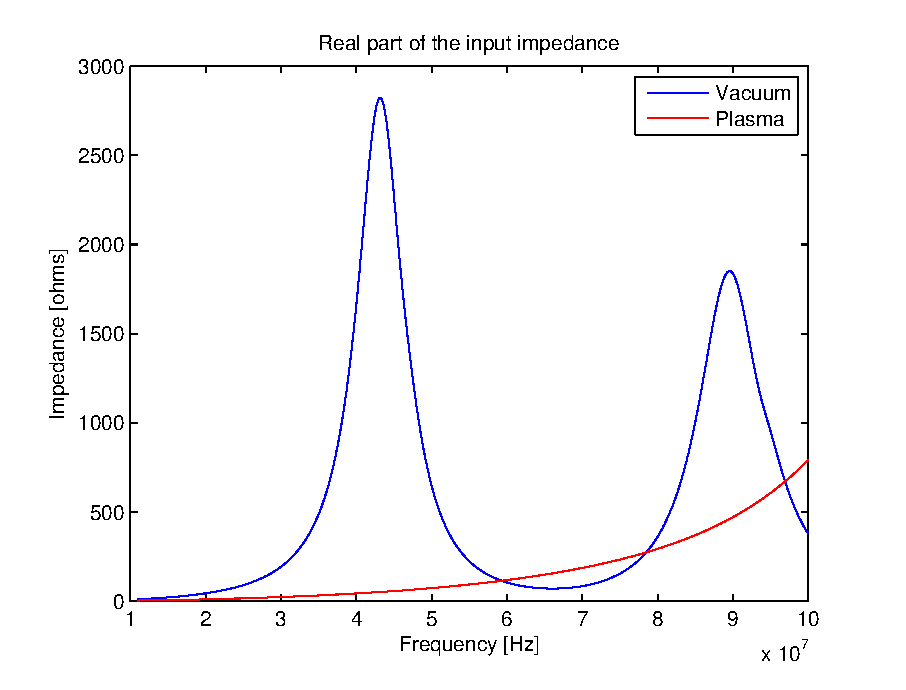
\includegraphics[width=11.5cm]{DissPics/impedance_dipole_fixed_rel.eps}
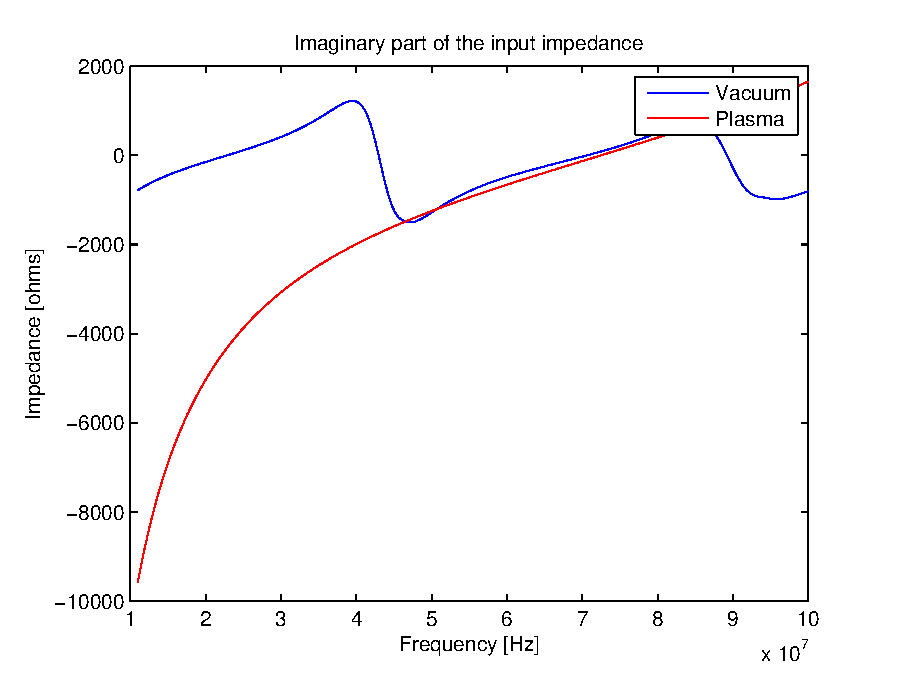
\includegraphics[width=11.5cm]{DissPics/impedance_dipole_fixed_rel_imag.eps}
 \caption{Impedance curves of the dipole with and without plasma. Fixed $\frac{\omega_{pe}^2}{\omega^2}=0.9$ }\label{fig:imps_fixed}
 \end{center}
\end{figure}

Figure \ref{fig:imps_10MHz} shows the curves when the electron plasma frequency is set to $10MHz$ which is a realistic situation. The influence has the effect to shift the resonance to a higher frequency which is the result of the increased wavelength at a given frequency.

\begin{figure}
\begin{center}
 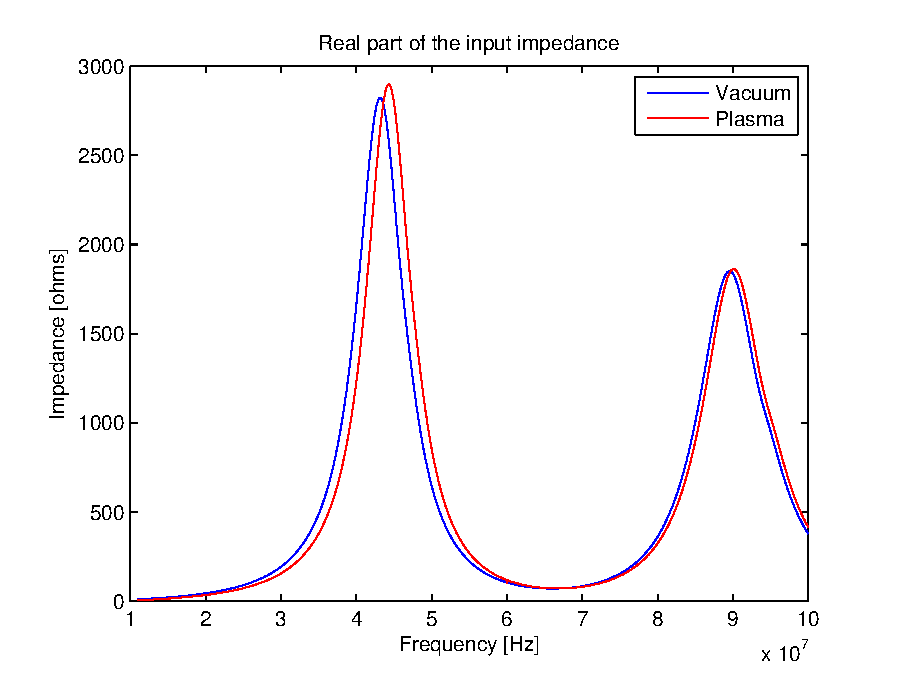
\includegraphics[width=11.5cm]{DissPics/impedance_dipole_fixed_abs.eps}
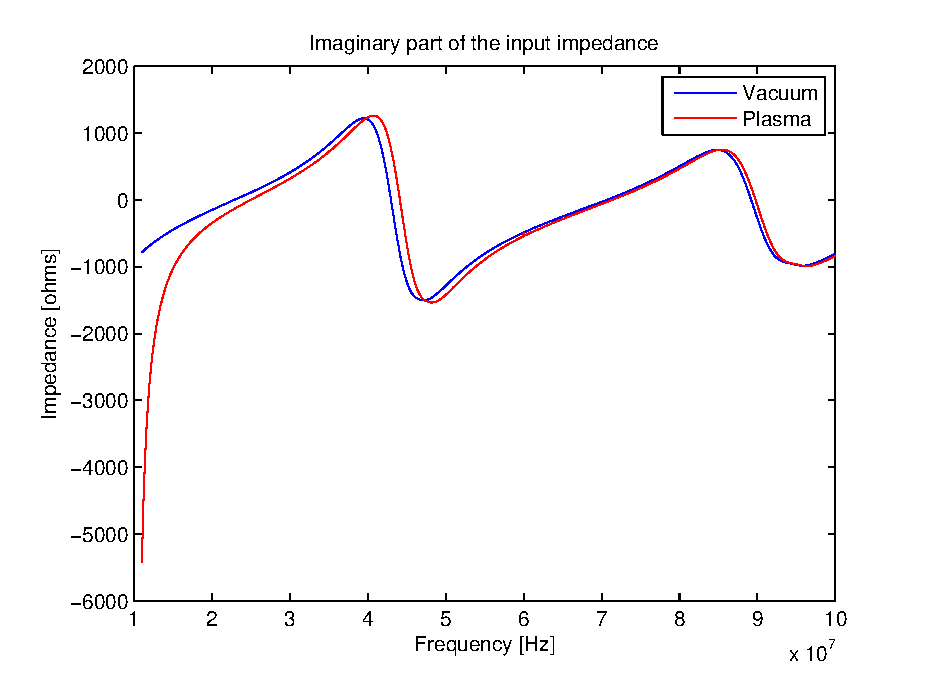
\includegraphics[width=11.5cm]{DissPics/impedance_dipole_fixed_abs_imag.eps}
 \caption{Impedance curves of the dipole with and without plasma. $\omega_{pe}=10MHz$ }\label{fig:imps_10MHz}
 \end{center}
\end{figure}

\subsection{The dipole in cold isotropic plasma}
The final step when investigating the influence of the effect of plasma on the transmission properties of the dipole using the cold isotropic plasma model is to combine both effects. The current distribution and the calculation of the electric field pattern is performed, using the algorithm which includes the plasma effects. The results of the former two sections leave no doubt that the inclusion of the plasma effect will have a dramatic effect on the field pattern. This, in turn, can be used to expect a change in the direction of the effective length vectors of the antennas of a complicated body, as for example a spacecraft. This issue will be dealt with in the next chapter.\\

To illustrate the change of the pattern, the plots of a dipole under the $\frac{3}{2}\lambda$ resonance condition is shown in vacuum as well as in plasma in Figure \ref{fig:NF3halbelambdaMHz}.

\begin{figure}
\begin{center}
  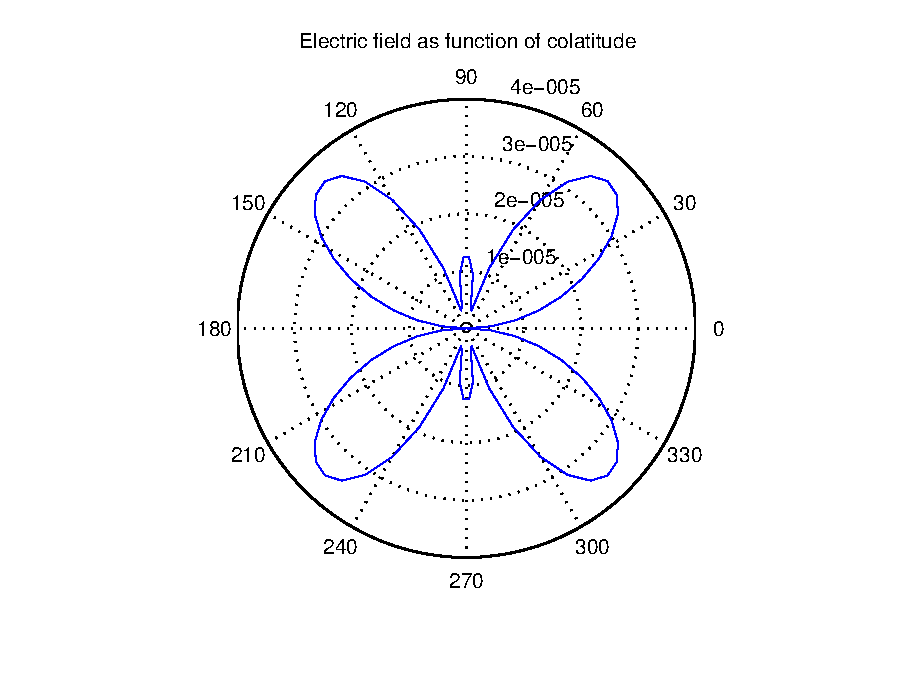
\includegraphics[width=11.5cm]{DissPics/NFvac10000m3halbelambdaMHz.eps}
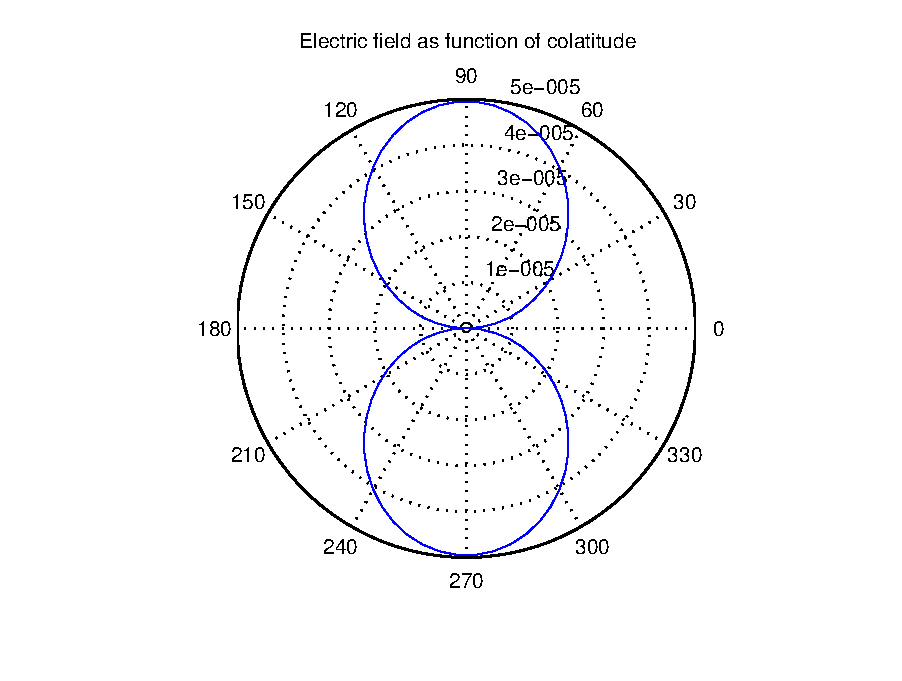
\includegraphics[width=11.5cm]{DissPics/NFvac10000m3halbelambdaMHz_p.eps}
  \caption{Electric field strength $[Vm^{-1}]$ at 10000m distance in vacuum (top) and in plasma at $\frac{3}{2}\lambda$ resonance condition (bottom)}\label{fig:NF3halbelambdaMHz}
\end{center}
\end{figure}

\chapter{Calculation of the Stereo spacecraft antenna properties}
In this chapter the effect of space plasma will be included in the calculation of antenna properties of actual spacecraft antennas. This is only possible for some simple cases. The standard antenna software packages do not allow for anisotropic dielectric tensors, the antenna calculation routines written by the author do not deal with complicated antenna structures which could resemble a spacecraft.\\

Some software packages do, however, allow dielectric constants of varying magnitude including the possibility of being complex. Thus it is possible to compute the value of the relative permittivity according to the plasma model and conditions and then include this value in the input parameters when calling the calculation routine. This pre-patch computation is done in the Matlab routine calling the actual software.\\

The spacecraft to be used for this test is the STEREO A spacecraft. The reason for this is that there exists a good wire and patch model as well as experimental results and actual measured data. Additionally the author of this doctoral thesis has some experience with regard to antenna calibration with this spacecraft.

\section{Cold isotropic plasma}
The first approach to be tested with the real spacecraft is the cold plasma model. As derived in former chapters the way the cold isotropic plasma manifests itself in the model is the relative permittivity. It is real and has a magnitude between zero and one ($0 \leq \mid \epsilon \mid \leq1$). The value one is modeling the vacuum case while the permittivity becomes smaller for plasma. Its actual value depends on the resonance frequencies and thus on the density of the electrons and to a smaller extent of the ions.\\

The software to be used in this section is CONCEPT II in combination with wires. The relative permittivity can be selected and put in, in form of modulus and argument, where the latter is always zero in this section because, as mentioned before, the permittivity in this simple cold plasma model is real.\\


\subsection{The effect on the antenna impedances}

\begin{figure}
\begin{center}
  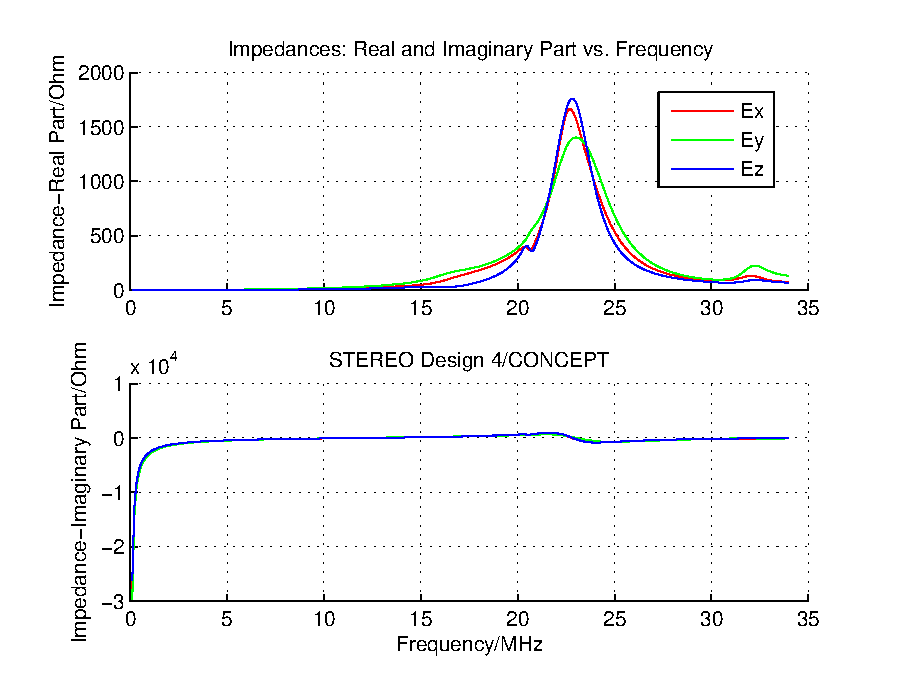
\includegraphics[width=11.5cm]{DissPics/impedance_stereo_vac.eps}
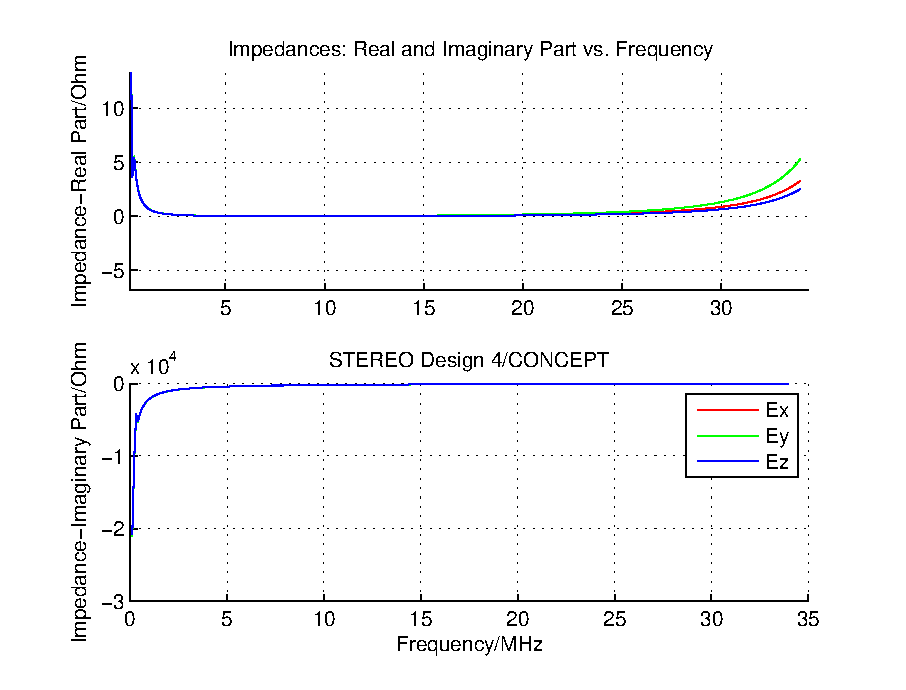
\includegraphics[width=11.5cm]{DissPics/impedance_stereo_pl.eps}
  \caption{The impedance of the S/WAVES antennas in vacuum (top) in relation to cold plasma with $\epsilon_r=0.1$ (bottom)}\label{fig:imp_stereo}
  \end{center}
\end{figure}

Figures \ref{fig:imp_stereo} show the results of these calculations, performed with a constant relative permittivity of $0.1$. The effect on the impedance curve shows the same behavior as for the dipole. The resonance is shifted to a higher frequency, in this particular case even out of the range of the graph (\ref{fig:imp_stereo}, bottom). The curves for the three antennas are so close together at some parts, that they appear as single line. Since Matlab draws one line after another, the final color of the line is blue, the color of the last curve to be drawn on top of the others. The same is true for the following Figures.\\

\begin{figure}
\begin{center}
  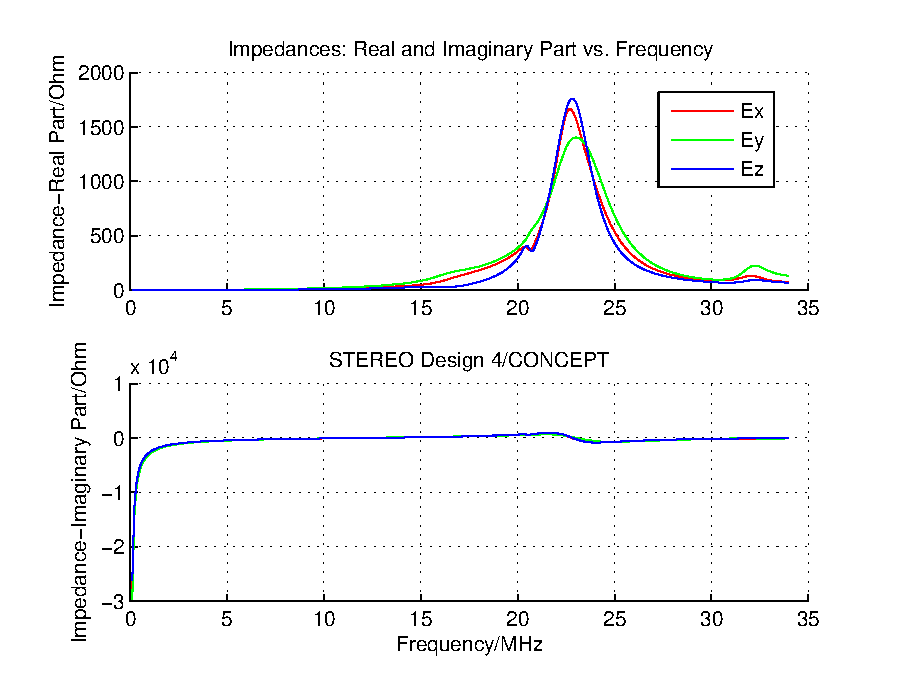
\includegraphics[width=11.5cm]{DissPics/impedance_stereo_vac.eps}
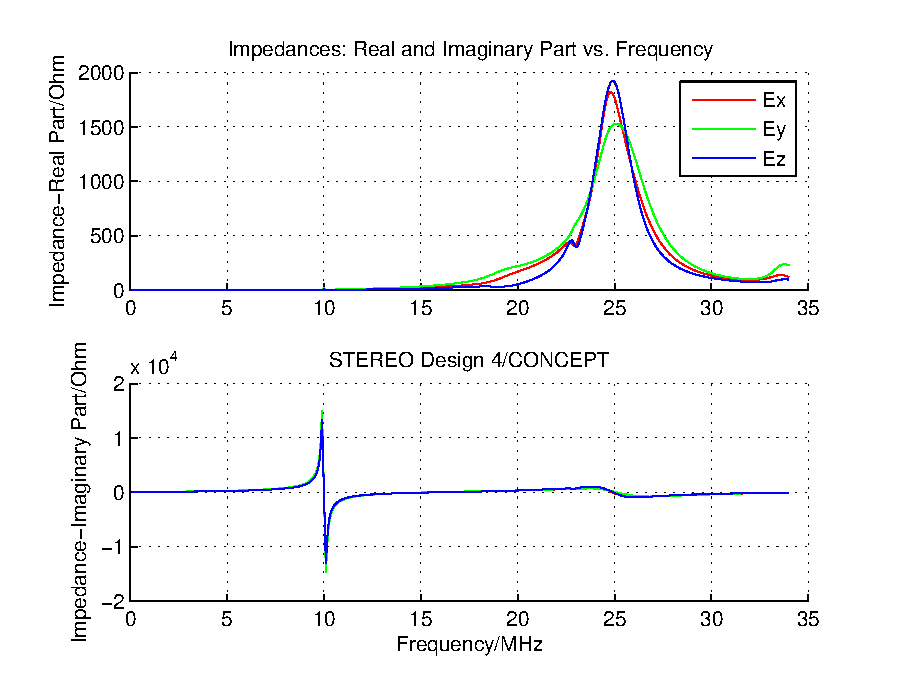
\includegraphics[width=11.5cm]{DissPics/impedance_stereo_pl_fix.eps}
  \caption{The impedance of the S/WAVES antennas in vacuum (top) in relation to cold plasma with $f_{pe}=10MHz$ (bottom)}\label{fig:imp_stereo_fix}
  \end{center}
\end{figure}

Figures \ref{fig:imp_stereo_fix} show the same calculation with a fixed electron plasma frequency of 10MHz. Only the part of the graph above 10MHz is relevant. The model is not valid at the lower frequency range. Figure \ref{fig:imp_stereo_fix_zoom} shows a small rise of the real and imaginary part of the impedance curve when tending towards the plasma resonance.

\begin{figure}
\begin{center}
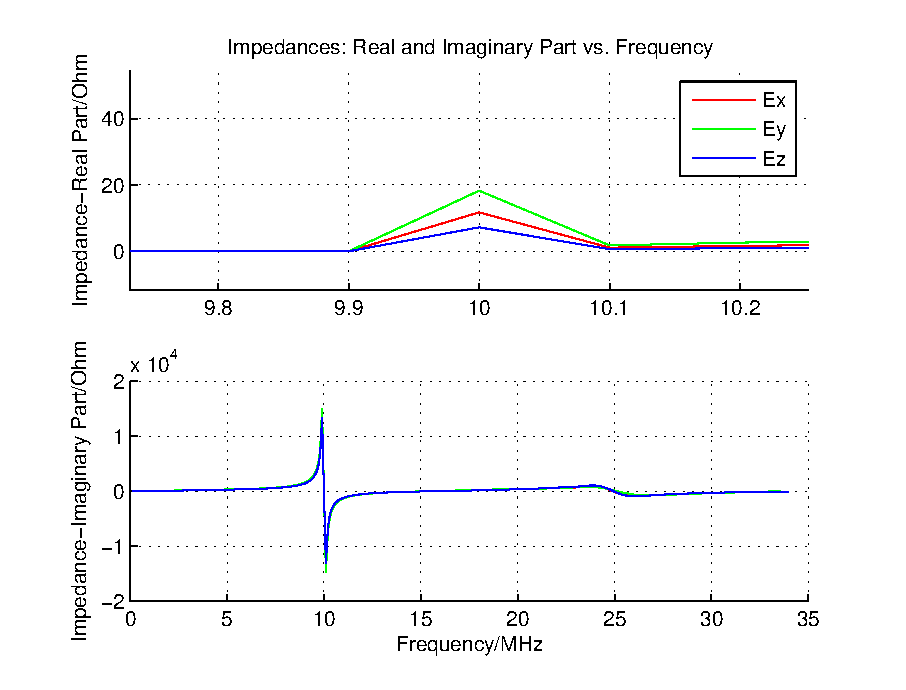
\includegraphics[width=11.5cm]{DissPics/impedance_stereo_pl_fix_zoom.eps}
  \caption{The impedance of the S/WAVES antennas in cold plasma with $f_{pe}=10MHz$, zooming into the frequency range around 10MHz}\label{fig:imp_stereo_fix_zoom}
\end{center}
\end{figure}

\begin{figure}
\begin{center}
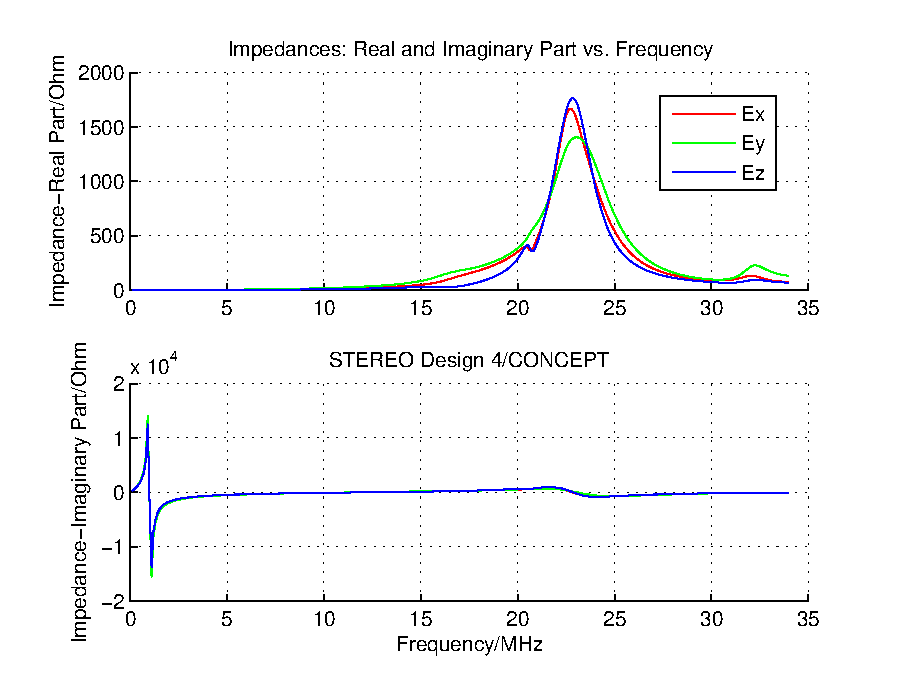
\includegraphics[width=11.5cm]{DissPics/impedance_stereo_pl_1mhz.eps}
  \caption{The impedance of the S/WAVES antennas in cold plasma with $f_{pe}=1MHz$}\label{fig:imp_stereo_1MHZ}
\end{center}
\end{figure}

\subsection{The effect on the effective length vectors}
Computing the effective length vectors using the cold plasma permittivity results in a slightly longer effective length vector. The directions are not altered very much. As an example the quasistatic effective length vectors of the STEREO antennas are given in Tables \ref{tab:heff_vacuum} and \ref{tab:heff_cold_plasma}. In both cases a frequency of $300kHz$ is used, which is a typical value when investigating the behavior of an antenna in the quasistatic limit. At the first table, vacuum is used as the surrounding medium, while a cold isotropic plasma model is used for comparison (second table).


\begin{table}
\begin{center}
\caption{Effective length vectors in vacuum: $f=300kHz$}
\label{tab:heff_vacuum}
\begin{tabular}{|c|c|c|c|}
 \hline
 & $length/m$ & $\zeta/^\circ$ & $\xi/^\circ$ \\
\hline
$E_x$ & $1.35$ & $119.9$ & $-135.3$ \\
$E_y$ & $1.64$ & $114.4$ & $127.3$ \\
$E_z$ & $1.09$ & $124.7$ & $15.5$ \\
\hline\end{tabular}
\end{center}
\end{table}



\begin{table}
\begin{center}
\caption{Effective length vectors in cold plasma: f=300kHz, $f_{pe}=100kHz$}
\label{tab:heff_cold_plasma}
\begin{tabular}{|c|c|c|c|}
 \hline
 & $length/m$ & $\zeta/^\circ$ & $\xi/^\circ$ \\
\hline
$E_x$ & $1.26$ & $119.6$ & $-135.0$ \\
$E_y$ & $1.53$ & $114.1$ & $127.2$ \\
$E_z$ & $1.02$ & $124.3$ & $15.2$ \\
\hline\end{tabular}
\end{center}
\end{table}

\chapter{The physics of the plasma sheath}
The antennas of a spacecraft are electromagnetically coupled to each other, to other parts of the spacecraft, and to the surrounding space plasma. The coupling can often be described by a
combination of resistivity and capacitance, which are the mutual resistance and capacitances when describing the interaction between antennas, the base resistance and capacitances when describing the interaction between the antennas and the hull, and finally the sheath resistance $R_s$ and sheath capacitance $C_s$ when treating the coupling between the antennas and the plasma (see Fig. \ref{fig_schaltplan}). The resistive coupling dominates at frequencies below the typical plasma frequencies and the capacitive coupling  dominates at high frequencies \cite{gurnett98}. \\

When spaceborn, two or three (in case of an existing photoelectron current contribution) different currents act on the conduction surface of the spacecraft, the current of positively charged ions and thermal electrons are flowing towards the surface, and, if parts of the spacecraft are exposed to sunlight, the current of photoelectrons is flowing away from the surface. Because the velocity of the thermal electrons is higher than the velocity of the ions, the spacecraft potential of a spacecraft which is not illuminated from sunlight, or is moving through a dense plasma where the current of the photoelectrons is negligible in comparison to the current due to the thermal electrons, is negative. If the photoelectron current dominates, which is usually the case in rarefied plasma, the thermal electron current, the spacecraft, and the spacecraft antennas, will be charged positively.

\begin{figure}
\includegraphics[width=12cm]{DissPics/schaltplan.eps}\\
\caption{Circuit diagram of an antenna system \cite{bale07}}
\label{fig_schaltplan}
\end{figure}


\section{Antenna-plasma coupling on a negatively charged spacecraft}
Due to the negative charge of the spacecraft, an ion sheath will be created, a zone which is mostly depleted of electrons. The thermal electrons have to cross a potential difference which results in preventing the less energized electrons to reach the surface. The positively charged ions are attracted, so their current will increase. The photoelectron current, which consists of electrons created by the photoelectric effect due to incident sunlight, does not depend on the thickness of the sheath or the potential of the spacecraft. A steady state condition is eventually reached, where the total current is zero.

\begin{equation}
I_{ant}+I_{th}+I_i+I_{ph}=0
\end{equation}

$I_{ant}$ is the current flowing from the antenna to the receiver, $I_{th}$ is the current of the thermal electrons, $I_i$ is the ion current and $I_{ph}$ is the photoelectron current. The photoelectron current is equal to the photoelectron production rate because due to the negatively charged spacecraft all photoelectrons cross the sheath and eventually reach the space plasma. It can be estimated by

\begin{equation}
I_{ph}=i_{ph}A_\phi
\end{equation}

where $i_{ph}$ is the photoelectron saturation current which has the dimensions $Am^{-2}$. In solar wind, it can be estimated as $i_{ph}\sim 10^{-4} Am^{-2}$ according to \cite{fahleson67}, while  \cite{grard73} gives $2\cdot 10^{-5}Am^{-2}$ as appropriate value. $A_\phi$ is the projected area of the antenna, which one can estimate as length of the antenna times the diameter times a factor $A_{rel}$ due to the angle of the antenna in relation to the direction of the sun and the part of the antenna which is in the shadow of the spacecraft hull, which is estimated crudely as $0.5$ for most spacecraft. A current is defined which brings a positive charge to the antenna as positive. Hence the photoelectron current, which consists of negatively charged electrons leaving the antenna, is positive.

\begin{equation}\label{eq:photo_current}
I_{ph} \sim A_{rel} i_{ph}ld
\end{equation}


$l$ is the length of the cylindrical antenna, while $d$ is the diameter. A detailed analysis of the thermal electron current, shape of the potential or charge density distribution along the thickness of the sheath makes the solution of Poisson's equation necessary. The one-dimensional distribution function of the electrons in the sheath can be written as

\begin{equation}
    f_e(x,v)=\frac{\bar{n}_e}{\sqrt{\frac{2 \pi \kappa T_e}{m_e}}}e^{-\frac{\varepsilon}{\kappa T_e}}
\end{equation}

postulating a Maxwellian distribution and a steady state condition. The unit would be $[m^{-6}s^3]$. $\bar{n}_e$ is the mean electron density. There exist investigations for a monokinetic and monoenergetic distribution function but it seems a Maxwellian distribution is closer to reality. $\varepsilon=\frac{1}{2}m_e v^2-e\phi(x)$ is the conserved energy of an electron, where $\phi$ is the potential at point x. The potential has the following boundary conditions.

\begin{eqnarray}
\phi(0)&=&V\\
\phi(\infty)&=&0
\end{eqnarray}

In this section the spacecraft potential V is supposed to be negative in relation to the surrounding plasma. This can be the case when a sufficient strong solar radiation is not present. Spacecraft operating in such an environment often are not electromagnetically coupled to the space plasma because the particle density around the spacecraft and the antennas is not high enough. A sheath can not form.\\

The particle density can be calculated by taking the zeroth moment of the distribution function (\ref{velocity_moment_number_density}).

\begin{eqnarray}
    n_e(x)&=&\int_{-\infty}^\infty f_e(x,v)dv\\
&=&\int_{-\infty}^\infty \frac{\bar{n}_e}{\sqrt{\frac{2 \pi \kappa T_e}{m_e}}}e^{-\frac{\frac{1}{2}m_e v^2-e\phi(x)}{\kappa T_e}}dv\\
&=&\frac{\bar{n}_e}{\sqrt{\frac{2 \pi \kappa T_e}{m_e}}} e^{\frac{e\phi(x)}{\kappa T_e}} \int_{-\infty}^\infty e^{-\frac{\frac{1}{2}m_e v^2}{\kappa T_e}}dv \label{eq:standard_integral}\\
&=&\frac{\bar{n}_e}{\sqrt{\frac{2 \pi \kappa T_e}{m_e}}} e^{\frac{e\phi(x)}{\kappa T_e}} \sqrt{\frac{2\pi \kappa T_e}{m_e}}\\
&=&\bar{n}_e e^{\frac{e\phi(x)}{\kappa T_e}}
\end{eqnarray}

The integral in (\ref{eq:standard_integral}) is a standard Gau\ss'ian error integral. The solution can be looked up in an integral table. The thermal current incident on the spacecraft can be computed by taking the first velocity moment of the distribution function, which yields the bulk speed multiplied by the particle density.


\begin{eqnarray}
    j_e(x)&=&-e\int_{-\infty}^\infty v f_e(x,v)dv\\
&=&-e\int_{-\infty}^\infty \frac{\bar{n}_e}{\sqrt{\frac{2 \pi \kappa T_e}{m_e}}}v e^{-\frac{\frac{1}{2}m_e v^2-e\phi(x)}{\kappa T_e}}dv\\
&=&-\frac{e \bar{n}_e}{\sqrt{\frac{2 \pi \kappa T_e}{m_e}}} e^{\frac{e\phi(x)}{\kappa T_e}} \int_{-\infty}^\infty v e^{-\frac{\frac{1}{2}m_e v^2}{\kappa T_e}}dv\\
&=&-e \bar{n}_e \sqrt{\frac{\kappa T_e}{2\pi m_e}} e^{\frac{e\phi(x)}{\kappa T_e}}
\end{eqnarray}

So the thermal electron current can be estimated as

\begin{equation}\label{eq:thermal_electron_current}
I_e=-e\bar{n}_e A \sqrt{\frac{\kappa T_e}{2\pi m_e}}e^{\frac{eV}{\kappa T_e}}
\end{equation}

$A$ is the surface area of the antenna, i.e. $ld\pi$ in the case of a cylindrically shaped antenna. The Boltzmann factor takes care that only these electrons exhibiting enough energy to cross the potential difference of the sheath, will reach the surface of the antenna and contribute to the thermal electron current. Using the Boltzmann factor implies a Maxwellian energy distribution which is supported by measurements \cite{grard73}. Ignoring the influence of the relatively immobile ions, the thermal current and the photoelectron current can be equated to estimate the floating potential ($I=0$) of the antenna ((\ref{eq:thermal_electron_current})+(\ref{eq:photo_current})=0):

\begin{equation}
V=\frac{\kappa T_e}{e} \ln\left[\frac{i_{ph} A_{\textrm{rel}}}{e\bar{n}_e  \pi} \sqrt{\frac{2 m_e}{\kappa T_e}}\right]
\end{equation}

This equation is a very rough estimation for antennas of cylindrical shape, ignoring the effect of the ion current and the finite velocity of the spacecraft. Measurements from former space mission have shown that the potential is rarely above 10V. A more accurate equation can be found by taking into account the ion current. All ions reach the surface, because they are attracted by the negatively charged spacecraft. So the ion flux $n_i(x)v_i(x)$ has to be conserved, postulating cold ions which move towards the spacecraft with a speed corresponding to the average kinetic speed of the real plasma. Since the ions accelerate when falling down the potential slope, they become faster and their density decreases with $n_i(x)\propto v_i(x)^{-1}$. Also their energy is conserved.

\begin{equation}
    \frac{1}{2}m_i\bar{v}_i^2=\frac{1}{2}m_iv_i(x)^2+e\phi(x)
\end{equation}

$\bar{v}_i$ is the kinetic speed of the ions. So

\begin{equation}
    v_i(x)=\sqrt{\bar{v}_i^2-\frac{2e\phi(x)}{m_i}}
\end{equation}

Using the conservation of the ion flux, a relation between the number density and the potential can be found.

\begin{equation}
    n_i(x)=\frac{\bar{n}_i}{\sqrt{1-\frac{2e\phi(x)}{m_i\bar{v}_i^2}}}
\end{equation}


Hence the ion current can be estimated as

\begin{equation}
    I_i(x)=eld\pi n_i(x)v_i(x)=eld\pi \frac{v_i(x) \bar{n}_i}{\sqrt{1-\frac{2e\phi(x)}{m_i\bar{v}_i^2}}}
\end{equation}

To find the ion current at the surface, one could set the spatial variable x to zero. But due to the required flux conservation, one can simply write

\begin{equation}
    I_i(x)=eld\pi \bar{n}_i\bar{v}_i
\end{equation}

and a new relation for the spacecraft potential can be found, this time including the effect of the ions.

\begin{equation}
V=\frac{\kappa T_e}{e} \ln\left[\left(\frac{i_{ph} A_{\textrm{rel}}}{e\bar{n}_e  \pi}+\bar{v}_i\right) \sqrt{\frac{2\pi m_e}{\kappa T_e}}\right]
\end{equation}

Quasi-neutrality was postulated in this equation. The effect of the ion current, however, is very small. Similar considerations can be used for the photoelectrons.

\begin{equation}
    \frac{1}{2}m_e\bar{v}_{ph}^2-eV=\frac{1}{2}m_e v_{ph}(x)^2-e\phi(x)
\end{equation}

This results in

\begin{equation}
    v_{ph}(x)=\sqrt{\bar{v}_{ph}^2-\frac{2e}{m_e}\left(V-\phi(x)\right)}
\end{equation}

and

\begin{equation}
    n_{ph}(x)=\frac{\bar{n}_{ph}}{\sqrt{1-\frac{2e}{m_e\bar{v}_{ph}^2}\left(V-\phi(x)\right)}}
\end{equation}

The kinetic velocity can be computed from the average photoelectron energy which is known to be $1.5eV$, and the particle density can be computed with the relation

\begin{equation}
j_{ph}(0) = i_{ph}=e \bar{v}_{ph} \bar{n}_{ph}
\end{equation}

at $x=0$, i.e. at the surface. To calculate the structure of the potential inside the sheath, Poisson's equation has to be employed. The one dimensional version dealing with the case of a flat surface can be written as Poisson's equation

\begin{equation}
    \frac{d^2 \phi(x)}{dx^2}=-\frac{e(n_i(x)-n_{ph}(x)-n_e(x))}{\epsilon_0}
\end{equation}

Inside the sheath of a negatively charged body the charge density of the ions is expected to be larger than the charge density of the electrons, because the body repels the light electrons creating an electron depletion zone. Therefore a convex structure of the potential is expected. After substituting the relevant particle densities, one gets

\begin{equation}
    \frac{d^2 \phi(x)}{dx^2}=-\frac{e}{\epsilon_0}\left(\frac{\bar{n}_i}{\sqrt{1-\frac{2e\phi(x)}{m_i\bar{v}_i^2}}}-
\frac{\bar{n}_{ph}}{\sqrt{1-\frac{2e}{m_e\bar{v}_{ph}^2}\left(V-\phi(x)\right)}}-\bar{n}_e e^{\frac{e\phi(x)}{\kappa T_e}}\right)
\end{equation}

The equation is non-linear and can therefore only be solved numerically. It can be simplified if the following conditions are true.

\begin{eqnarray}
% \nonumber to remove numbering (before each equation)
  e\phi(x) &\ll& m_i\bar{v}_i^2 \\
 e(V-\phi(x)) &\ll& m_e\bar{v}_{ph}^2 \\
 e\phi(x) &\ll& \kappa T_e
 \end{eqnarray}

Then the second term under each square root is very small and the equation can be approximated by a Taylor expansion. This condition, when the potential energy is small in relation to the kinetic and thermal energies of the particles, corresponds to the part of the sheath which is distant from the object, i.e. the spacecraft.

\begin{eqnarray}
% \nonumber to remove numbering (before each equation)
  \frac{1}{\sqrt{1-\frac{2e\phi(x)}{m_i\bar{v}_i^2}}} &\sim& 1+\frac{2e\phi(x)}{m_i\bar{v}_i^2} \\
\frac{1}{\sqrt{1-\frac{2e}{m_e\bar{v}_{ph}^2}\left(V-\phi(x)\right)}} &\sim& 1+\frac{2e\left(V-\phi(x)\right)}{m_e\bar{v}_{ph}^2} \\
e^{\frac{e\phi(x)}{kT_e}} &\sim& 1+\frac{e\phi(x)}{\kappa T_e}
\end{eqnarray}

Then

\begin{eqnarray}
    &&\frac{d^2\phi(x)}{dx^2}=-\frac{e}{\epsilon_0}\left(\bar{n}_i  \left(1+\frac{2e\phi(x)}{m_i\bar{v}_i^2}\right) \right.\\
    &&\left. -\bar{n}_{ph}\left(  1+\frac{2e\left(V-\phi(x)\right)}{m_e\bar{v}_{ph}^2}\right)-\bar{n}_e \left( 1+\frac{e\phi(x)}{\kappa T_e} \right) \right)\nonumber\\
&&=-\frac{e}{\epsilon_0}\left( (\bar{n}_i -  \bar{n}_{ph} -  \bar{n}_e ) \right. \nonumber\\
&& \left. + e\left( \frac{2\bar{n}_i \phi(x)}{m_i\bar{v}_i^2} +\frac{2\bar{n}_{ph}(V-\phi(x))}{m_e\bar{v}_{ph}^2}-\frac{\bar{n}_e \phi(x)}{\kappa T_e}\right)  \right)\nonumber\\
&&=-\frac{e}{\epsilon_0}\left( \left(\bar{n}_i -  \bar{n}_{ph} \left( 1+ \frac{2eV}{m_e\bar{v}_{ph}^2}\right)-  \bar{n}_e \right)\right.\nonumber \\
&& \left. + e\left( \frac{2\bar{n}_i}{m_i\bar{v}_i^2} +\frac{2\bar{n}_{ph}}{m_e\bar{v}_{ph}^2}-\frac{\bar{n}_e }{\kappa T_e}\right)\phi(x)  \right)  \nonumber
\end{eqnarray}
Hence
\begin{eqnarray}
 &&\frac{d^2\phi(x)}{dx^2}+\frac{e^2}{\epsilon_0}\left( \frac{2\bar{n}_i }{m_i\bar{v}_i^2} +\frac{2\bar{n}_{ph}}{m_e\bar{v}_{ph}^2}-\frac{\bar{n}_e }{\kappa T_e}\right)\phi(x) \\
 &&=-\frac{e}{\epsilon_0}\left( \bar{n}_i - \left( 1+ \frac{2eV}{m_e\bar{v}_{ph}^2}\right) \bar{n}_{ph} -  \bar{n}_e  \right)\nonumber
\end{eqnarray}

which can be solved analytically. To preserve the physical content of the original equation, the solution must be convex, which means that the term in the brackets on the left side must be smaller than zero (the potential is negative). Neglecting the photoelectrons and assuming quasi-neutrality, this means the condition

\begin{equation}
    \frac{m_i\bar{v}_i^2}{2} > \kappa T_e
\end{equation}

i.e. the mean kinetic energy of the ions must be greater than the thermal energy of the electrons. This is called the Bohm criterion. If no photoelectrons are present, the linearized differential equation is

\begin{eqnarray}
    \frac{d^2\phi(x)}{dx^2}&=&-\frac{e}{\epsilon_0}\left[\bar{n}_i  \left(1+\frac{2e\phi(x)}{m_i\bar{v}_i^2}\right)  -\bar{n}_e \left( 1+\frac{e\phi(x)}{\kappa T_e} \right) \right]
\end{eqnarray}

Assuming quasi-neutrality

\begin{eqnarray}
    \frac{d^2\phi(x)}{dx^2}&=&-\frac{e^2\bar{n}_0}{\epsilon_0}\left( \frac{2}{m_i\bar{v}_i^2}  - \frac{1}{\kappa T_e} \right)\phi(x)
\end{eqnarray}

The Bohm criterion has to be applied. The solution of this equation is

\begin{equation}
    \phi(x)=Ve^{-\frac{x}{\lambda_{sh}}}
\end{equation}

where

\begin{equation}
    \lambda_{sh}=\sqrt{\frac{\epsilon_0}{e^2\bar{n}_0}\left( \frac{2}{m_i\bar{v}_i^2}  - \frac{1}{\kappa T_e} \right)^{-1}}
\end{equation}

The thickness of the sheath can be estimated as

\begin{equation}
\delta=\lambda_{sh}
\end{equation}

Due to the Bohm criterion this value is similar to the Debye length of the thermal electrons, so the thickness of the plasma sheath of a negatively charged spacecraft without photoelectrons can be estimated as the magnitude of the electron Debye length to a first approximation. In rarefied plasma, the electron Debye length is too large to permit any effective coupling between antenna and space plasma. In this case the antenna-plasma coupling can only work if photoelectrons are present. If the photoelectron current outweighs the thermal electron current, the antenna/spacecraft is charged positively, changing the physics of the system. This case will be analyzed in the next section. The plasma resistance $R_s$ is the gradient of the V-I curve.

\begin{equation}
R_s=\frac{\partial V}{\partial I}
\end{equation}

In the case of a negatively charged antenna, it can be shown that

\begin{equation}
R_s=\frac{\kappa T_e}{e(I_{ph}+I_i)}
\end{equation}

at low frequencies \cite{gurnett98}, where $I_{ph}$ is the photoelectron current and $I_i$ the ion current. At high frequencies the resistive part of the plasma impedance can be neglected. The capacitance $C_s$ between the antenna and the plasma can be estimated by using the equation of a cylindrical capacitor.

\begin{equation}
C_s=l_a\frac{2\pi \epsilon_0}{\ln{\left( \frac{\delta}{r_a} \right)}}
\end{equation}

$l_a$ and $r_a$ are the length and the radius of the antenna, respectively.

\section{Antenna-plasma coupling on a positively charged spacecraft}
On a positively charged spacecraft, the number of generated photoelectrons exceeds the number of thermal electrons reaching the surface. Therefore the number of photoelectrons with an energy high enough to cross the sheath and enter the space plasma must be in balance to the thermal electrons. The thermal electrons are attracted to the surface so all of them reach the surface, while most of the photoelectrons will not be able to leave the sheath and fall back to the surface. They do not contribute to the photoelectron current. Hence, the distribution of the photoelectrons, which can be reasonably approximated as Maxwellian, has to be considered instead of the thermal electrons which results in

\begin{equation}
I_e=-en_e dl\pi \sqrt{\frac{\kappa T_e}{2\pi m_e}}
\end{equation}

and

\begin{equation}\label{eq:ph_current_positive_sc}
I_{ph} = A_{rel} i_{ph}ld e^{-\frac{eV}{\kappa T_{ph}}}
\end{equation}

$T_{ph}$ is the kinetic temperature of the photoelectrons which can be taken to be $1.5eV$ in solar wind conditions at one AU \cite{grard73}. The floating potential can be derived in a similar way as in the case of a negative potential by equating the currents $(I_e+I_{ph}=0)$.

\begin{equation}\label{eq:volt_positive_sc}
 V=-\frac{\kappa T_{ph}}{e}\ln{\left[\frac{en_e \pi}{A_{rel} i_{ph}} \sqrt{\frac{\kappa T_e}{2\pi m_e}}\right]}
\end{equation}

A positively charged spacecraft is covered with a sheet of photoelectrons. In a dynamical process photoelectrons are created in a rate of $i_{ph}\times illuminated area$. Not all electrons reach the environmental plasma, only those which have an energy large enough to cross the potential difference of the plasma sheath. The electrons with lower energy fall back to the surface and are absorbed again. The fraction of the photoelectrons which are unable to leave the spacecraft is


\begin{equation}
\frac{1}{ V } \int_0^V e^{-\frac{e\phi}{\kappa T_{ph}}} d\phi=\frac{1}{ V }\left[ -\frac{\kappa T_{ph}}{e}e^{-\frac{e\phi }{\kappa T_{ph}}}\right]_0^V=1-e^{-\frac{eV}{\kappa T_{ph}}}
\end{equation}

So the back flowing photoelectron current is

\begin{equation}
I_{ph,back} = A_{rel} i_{ph}ld (1-e^{-\frac{eV}{\kappa T_{ph}}})
\end{equation}

But since the photoelectrons escaping to the space plasma are replaced by thermal electrons, the total back flowing current at the surface of the antenna is the production rate on average. This must be the case such that the net charge of the antenna remains constant on a timescale which is large enough to balance the emission or absorption processes of individual particles.

\begin{equation}
I_{back} = I_{ph,back}+I_e \sim A_{rel} i_{ph}ld
\end{equation}


In a steady state condition, the average number density of electrons inside the sheath must be constant. The particle density due to the photoelectron current can be estimated by using the equation

\begin{equation}
\mathbf{j}=\bar{\mathbf{v}}nq
\end{equation}

where $\bar{v}=\sqrt{\frac{3kT}{m}}$ is the average velocity of the particle species. Hence on average the particle density due to the outgoing photoelectrons at the surface of the spacecraft is

\begin{equation}
n_{ph}(0)=\frac{j_{ph}(0)}{{\bar{v}_{ph}(0) q}}=\frac{j_{ph}(0)}{\bar{v}_{ph}(0)e}=\frac{A_{rel} i_{ph}ld}{dl\pi\bar{v}_{ph}(0)e}=\frac{A_{rel} i_{ph}}{\pi\bar{v}_{ph}(0)e}
\end{equation}

The total electron density is twice the density of the outgoing photoelectrons.

\begin{equation}\label{ne0}
n_{e,tot}(0)=\frac{2 A_{rel} i_{ph}}{\pi\bar{v}_{ph}(0)e}
\end{equation}

An interesting result is that the particle density is independent of the diameter and length of the antenna. The thickness of the sheath can be estimated as

\begin{equation}
    \delta \sim \lambda_{ph}=\sqrt{\frac{\epsilon_0 \kappa T_{ph}}{n_{totph}(0) e^2}}
\end{equation}

As in the last section, for a fully consistent theory which provides the particle and potential distribution along the thickness of the sheath, Poisson's equation has to be solved. The thermal electron particle density can be found in accordance with the ion particle density of the negatively charged spacecraft which results in

\begin{equation}
    n_e(x)=\frac{\bar{n}_e}{\sqrt{1+\frac{2e\phi(x)}{m_e\bar{v}_e^2}}}
\end{equation}

while the density of the photoelectrons is found like the density of the thermal electrons in the case of a negatively charged spacecraft, since the photoelectrons are postulated to have a Maxwell-Boltzmann distribution.

\begin{equation}\label{eq:photoelectron_density}
    n_{ph}(x)=2n_{ph}(0) e^{-\frac{e(V-\phi(x))}{\kappa T_{ph}}}
\end{equation}

The factor of 2 is necessary to include the photoelectrons which are falling back to the surface. It can be reasonably postulated that the heavy ions are not disturbed by the potential variation inside the sheath.

\begin{equation}
    n_i(x)=\bar{n}_i
\end{equation}

In a one-dimensional simplification which postulates a homogeneous sheath above a flat surface, it could be written as

\begin{equation}\label{eq:poisson}
    \frac{d^2 \phi(x)}{dx^2}=-\frac{e}{\epsilon_0}\left( \bar{n}_i -n_{ph}(x)-n_{e}(x) \right)
\end{equation}

Substituting for $n_{ph}$ and $n_e$ gives

\begin{equation}
    \frac{d^2 \phi(x)}{dx^2}-\frac{2en_{ph}(0)}{\epsilon_0} e^{-\frac{e(V-\phi(x))}{\kappa T_{ph}}}-\frac{e\bar{n}_e}{\epsilon_0\sqrt{1+\frac{2e\phi(x)}{m_e\bar{v}_e^2}}} =-\frac{e\bar{n}_i }{\epsilon_0}
\end{equation}

This equation is non-linear again and can only be solved by numerical methods. Two boundary conditions are needed, which would be the potential at the surface(V), and the potential at infinity(0). The equation can be linearized by approximating it with a Taylor polynomial.

\begin{eqnarray}
% \nonumber to remove numbering (before each equation)
  \frac{1}{\sqrt{1+\frac{2e\phi(x)}{m_e\bar{v}_e^2}}} &\sim& 1-\frac{2e\phi(x)}{m_e\bar{v}_e^2} \\
e^{\frac{e\phi(x)}{kT_e{ph}}} &\sim& 1+\frac{e\phi(x)}{\kappa T_{ph}}
\end{eqnarray}

Hence

\begin{equation}
    \frac{d^2 \phi(x)}{dx^2}-\frac{2en_{ph}(0)}{\epsilon_0} e^{-\frac{eV}{\kappa T_{ph}}}\left( 1+\frac{e\phi(x)}{\kappa T_�{ph}} \right)-\frac{e\bar{n}_e}{\epsilon_0}\left( 1-\frac{2e\phi(x)}{m_e\bar{v}_e^2}\right) =-\frac{e\bar{n}_i }{\epsilon_0}
\end{equation}

Assuming quasi-neutrality

\begin{equation}
    \frac{d^2 \phi(x)}{dx^2}-\frac{2en_{ph}(0)}{\epsilon_0} e^{-\frac{eV}{\kappa T_{ph}}}\left( 1+\frac{e\phi(x)}{\kappa T_{ph}} \right)+\frac{2e^2\bar{n}_0}{\epsilon_0 m_e\bar{v}_e^2} \phi(x)=0
\end{equation}

\begin{equation}
   \frac{d^2 \phi(x)}{dx^2}-\frac{2e^2}{\epsilon_0}\left(\frac{n_{ph}(0)}{ \kappa T_{ph}} e^{-\frac{eV}{\kappa T_{ph}}}  -\frac{\bar{n}_0}{ m_e\bar{v}_e^2}\right) \phi(x)=\frac{2en_{ph}(0)}{\epsilon_0} e^{-\frac{eV}{\kappa T_{ph}}}
\end{equation}

As in the last section the approximation is valid if the potential energy of the particles is low in relation to the thermal energy, which is to be expected near the boundary of the sheath. The solution is an exponential function to which a constant has to be added. Due to physical reasoning only the part which the negative exponent remains. It has to be emphasized that the boundary conditions are not fulfilled in this approximation. This is not relevant, since the approximation is not valid at the boundaries, therefore it can not be expected to yield correct results at these points. The shielding distance could be defined as

\begin{equation}\label{eq:sheath_debye_length}
    \lambda_{\textrm{sh}}=\left[\frac{2e^2}{\epsilon_0}\left(\frac{n_{ph}(0)}{ \kappa T_{ph}} e^{-\frac{eV}{\kappa T_{ph}}}  -\frac{\bar{n}_0}{ m_e\bar{v}_e^2}\right)\right]^{-\frac{1}{2}}
\end{equation}


Using a cylindrical polar coordinate system, eq. (\ref{eq:poisson}) would be altered to

\begin{equation}\label{eq:poisson_cyl}
    \frac{1}{r}\frac{d}{dr}\left( r\frac{d \phi(r)}{dr}\right)=-\frac{e}{\epsilon_0}\left( \bar{n}_i -n_{ph}(r)-n_{e}(r) \right)
\end{equation}

which results in

\begin{equation}\label{eq:poisson_cyl_2}
    \frac{1}{r}\frac{d}{dr}\left( r\frac{d \phi(r)}{dr}\right)-\frac{2en_{ph}(0)}{\epsilon_0} e^{-\frac{e(V-\phi(r))}{\kappa T_{ph}}} =-\frac{e\bar{n}_i }{\epsilon_0}
\end{equation}

and, using the Taylor expansion

\begin{equation}\label{eq:poisson_cyl_lin}
    \frac{1}{r}\frac{d}{dr}\left( r\frac{d \phi(r)}{dr}\right)-\frac{2e^2 n_{ph}(0)}{\kappa T_{ph} \epsilon_0} e^{-\frac{eV}{\kappa T_{ph}}}\phi(r) =\frac{e}{\epsilon_0}(2n_{ph}(0)e^{-\frac{eV}{\kappa T_{ph}}}-\bar{n}_i)
\end{equation}

The fact that the shape of the body discussed is now cylindrical, has no influence on the vanishing term at the right side of the equation, due to physical reasoning. So one can bring the equation into the form of a Sturm-Liouville problem.

\begin{equation}\label{eq:sturm-liouville}
   \frac{d}{dr}\left( r\frac{d \phi(r)}{dr}\right)-r\frac{2e^2 n_{ph}(0)}{\kappa T_{ph} \epsilon_0} e^{-\frac{eV}{\kappa T_{ph}}}\phi(r) =0
\end{equation}

By performing the outer differentiation is can be further reshaped into a modified Bessel's equation of order 0.

\begin{equation}\label{eq:bessel_de}
   R^2\frac{d^2 \Phi(R)}{dR^2}+ R\frac{d \Phi(R)}{dr} -R^2 \Phi(R) =0
\end{equation}

where

\begin{eqnarray}
    R&=&\lambda_{sh}r\\
    \Phi(R)&=&\phi(r)\\
    \lambda_{sh}&=&\sqrt{\frac{2e^2 n_{ph}(0)}{\kappa T_{ph} \epsilon_0} e^{-\frac{eV}{\kappa T_{ph}}}}
\end{eqnarray}

Due to the boundary conditions, the potential must vanish at infinity, a modified Bessel's function of second kind ($K$) is the correct solution. Hence the solution is

\begin{equation}
    \phi(\sqrt{C}r)=\Phi(R)=A K_0(R)=A K_0(\lambda_{sh}r)
\end{equation}

where A is a constant depending on the second boundary condition to ensure that the potential at the surface is equal to V.\\


The sheath resistance is connected to that part of the photoelectron current which leaves the sheath into the surrounding plasma encounters. This corresponds to the gradient of the voltage-current curve.

\begin{equation}
    R_s=\frac{dV}{dI_{ph}}
\end{equation}

Solving (\ref{eq:ph_current_positive_sc}) for V gives

\begin{equation}
V = -\frac{\kappa T_{ph}}{e} \ln{ \frac{I_{ph}}{A_{rel} i_{ph}ld}}
\end{equation}

Hence

\begin{equation}
    R_s=-\frac{\kappa T_{ph}}{eI_{ph}}
\end{equation}

The equation for the sheath capacitance is similar as for the ion sheath, with the difference that the sheath consists of electrons. Therefore the mean permittivity of an electron plasma has to be used.

\begin{equation}
C_s=l_a\frac{2\pi \epsilon_0 \bar{\epsilon}_r}{\ln{\left( \frac{\delta}{r_a} \right)}}
\end{equation}

Which version of the permittivity is to be used depends on the used model. In a simple cold isotropic model, equation (\ref{epsilon_plasma}) could be used with

\begin{equation}
    \bar{\epsilon}_r=\frac{1}{\delta}\int_{r'=0}^{r'=\delta}\left( 1-\frac{\omega_p(r')^2}{\omega^2}\right) dr'
\end{equation}

using the relevant equation for the electron plasma frequency and equation (\ref{eq:photoelectron_density}) for the photoelectron density.

\begin{eqnarray}
\int_{r'=0}^{r'=\delta}\left( 1-\frac{\omega_p(r')^2}{\omega^2}\right) dr'&=&\int_{r'=0}^{r'=\delta}\left( 1-\frac{n_e(r')e^2}{m_e\epsilon_0\omega^2}\right) dr'\\
&=&\int_{r'=0}^{r'=\delta}\left( 1-\frac{n_e(0)e^2}{m_e\epsilon_0\omega^2}e^{-\frac{eVr'}{\kappa T_{ph}\delta}}\right) dr'\\
&=&\delta+\left[\frac{\kappa T_{ph}\delta n_e(0)e^2}{eV m_e\epsilon_0\omega^2}e^{-\frac{eVr'}{\kappa T_{ph}\delta}}\right]_0^\delta \\
&=&\delta+\frac{\kappa T_{ph}\delta n_e(0)e}{V m_e\epsilon_0\omega^2}\left(e^{-\frac{eV}{\kappa T_{ph}}}-1 \right)
\end{eqnarray}

Hence,

\begin{equation}
    \bar{\epsilon}_r=1-\frac{\kappa T_{ph} n_e(0)e}{V m_e\epsilon_0\omega^2}\left(1-e^{-\frac{eV}{\kappa T_{ph}}} \right)
\end{equation}

Since the plasma sheath, positively or negatively charged, is irregularly shaped, the results of this and the former section have to be understood as more or less first order estimations. Resulting values should be checked against measurement results, which will be done for the STEREO spacecraft in the next section.

\section{Implementation of the sheath in numerical calibration of spacecraft antennas}
In this section the implementation of the results of the former section is shown, using STEREO as an example.

The spacecraft STEREO operates in solar wind conditions at 1AU. Therefore a photoelectron flux of $i_{ph}\sim 10^{-4} Am^{-2}$ can be used, which gives

\begin{equation}
I_{ph}=A_{rel} i_{ph}ld\sim 7.6 \cdot 10^{-6}A
\end{equation}

using $A_{rel}=\frac{1}{2}$ and the parameters of the SWAVES antennas, i.e. a length of 6 meters and a diameter of 1 inch (0.0254m). The thermal current is

\begin{equation}
I_e=-en_e d\pi \sqrt{\frac{\kappa T_e}{2\pi m_e}}\sim -2\cdot 10^{-7}A
\end{equation}

using an electron temperature of 10eV and an electron particle density of 5 electrons per cube centimeter. Clearly, the STEREO spacecraft must be positively charged because the photoelectron current is one order of magnitude higher than the thermal electron current. Using a photoelectron energy of 10eV, the potential difference can be estimated as

\begin{equation}
    V\sim5.5V
\end{equation}

according to equation (\ref{eq:volt_positive_sc}). This value is in accordance with the experience of former space missions and measurements (see \cite{kellogg01} for instance. By using this number in the Boltzmann factor it can be estimated that about $2.5\%$ of the produced photoelectrons have enough energy to cross the plasma sheath. The average speed of the photoelectron is $\bar{v}\sim 9\cdot 10^5 ms^{-1}$, resulting in a total particle density of $2\cdot10^8m^{-3}$. This, in turn results in a Debye length of $\lambda_{ph}\sim0.6m$ using the usual equation and $\lambda_{sh}\sim0.4m$ using equation (\ref{eq:sheath_debye_length}). Using these values gives a sheath resistance of

\begin{equation}
    R_s=0.2M\Omega
\end{equation}

and a capacitance of

\begin{equation}
    C_s=87pF
\end{equation}

\begin{figure}
\begin{center}
  \includegraphics[width=11.5cm]{DissPics/impedance_stereo_dipole_vac.eps}
\includegraphics[width=11.5cm]{DissPics/impedance_stereo_dipole_sheath.eps}
  \caption{The impedance of the S/WAVES $E_x-E_y$ dipole with inclusion of the plasma sheath (top) in relation to the case in vacuum (bottom)}\label{fig:imp_stereo_sheath_dipole}
  \end{center}
\end{figure}

\begin{figure}
\begin{center}
  \includegraphics[width=11.5cm]{DissPics/impedance_stereo_mono_vac.eps}
\includegraphics[width=11.5cm]{DissPics/impedance_stereo_mono_sheath.eps}
  \caption{The impedance of the S/WAVES $E_z$ monopole with inclusion of the plasma sheath (top) in relation to the case in vacuum (bottom)}\label{fig:imp_stereo_sheath_mono}
  \end{center}
\end{figure}


Figures \ref{fig:imp_stereo_sheath_dipole} and \ref{fig:imp_stereo_sheath_mono} show the impedance curves with and without plasma sheath on semi-logarithmic plots. It can be seen that the influence of the photoelectron sheath results in a shift of the second resonance to the right, i.e. to a higher plasma frequency. This corresponds to a shortening of the effective length vectors. The same behavior was seen in the former chapter, where a different method was developed and implemented, to allow for the plasma effect.



\chapter{Conclusion and outlook}
In this PhD thesis methods where investigated and shown to include the effects of space plasma in the numerical antenna calibration process. Only
frequencies above the characteristic plasma resonance frequencies where considered. In this frequency regime plasma effects are traditionally
ignored and the antennas are treated as in vacuum. Effects due to plasma are supposed to be so small that a detailed treatment seems not
to be necessary.\\

However the author of this thesis states that investigating this topic has certain importance and there are specific regimes and applications where the inclusion of the plasma in the computation is of value and can not be neglected. Such a regime
might be a dense space plasma which can be found in the magnetosphere of planets.\\

In the first Chapter the subject of the thesis was defined and introduced. The large second Chapter contains the theoretical framework and
formalism of electrodynamics and plasma electrodynamics on which the thesis is built. Since plasma electrodynamics is a rather new field of physics, many different styles and formalisms
co-exist in literature. Hence, before starting to work on the subject it was necessary to establish the formalism which is used consistently
throughout the thesis. A similar situation exists for antenna theory which is treated in Chapter three.\\

In hapter four the method for the numerical solution of the equations describing the antenna systems are introduced. While other methods,
like the finite difference time domain (FDTD) method, seem to be even more suitable for investigating antennas in plasma, the author has chosen the
method of moments (MOM) because it is the most widely used method for calibrating spacecraft antennas. A reason for this fact is because
complex geometrical structures can be represented most easily with this method.\\

Chapters 5 to 7 contain the actual investigations of the antennas in plasma. Chapter 5 deals with simple dipoles, using a simple 2D algorithm.
The solver was written by the author and the source code is printed in the appendix. First, the effect on the radiation pattern was
investigated, using equal current distributions. Then the effect of the plasma on current distribution and antenna impedance was investigated.
It was shown that the effect of the plasma on the computed results depends on frequency and resonance frequencies. For high frequencies the
plasma effect tends to zero, which is of course a well known result.\\

Chapter 6 deals with a real application, the antennas of the STEREO spacecraft. The effect of the plasma on antenna impedances and effective
length vectors was investigated, showing that the effects are rather small regarding the directions of the effective length vectors, but the
length of the effective lengths vectors are influenced considerably in a way that they are shorter than without plasma. The solver of CONCEPT II was used for the calculations in this chapter.\\

The final Chapter 7, uses a completely different approach to include the plasma effect in the antenna computations. It uses the model
of a plasma sheath which forms around all conducting bodies immersed in plasma. The sheath has a certain resistivity and capacity, which can
be applied to the equations describing the antenna behavior. This approach was investigated theoretically and applied to the STEREO spacecraft
antennas. The overall result is the same as when using the former approach, i.e. a decrease in length of the effective length vectors.\\

This thesis marks only the beginning of a possible investigation of the subject how to include the plasma effect into numerical antenna
calibration. There exists a wide field for future investigations. A possible next step would be to include anisotropy into the calculation and so the considering of an external magnetic field. The implementation would be to use the respective permittivity tensor instead of the isotropic permittivity which was used in this thesis. NEC 4 is able to perform computations of this kind, so it would be worthwhile to use this antenna calibration package for further investigations. A different approach would be to use a different modeling and solution process. In particular the FDTD method should be suitable for this kind of problem.\\

When numerical calculations of any kind are performed it is always mandatory to check the results either against known and proven results or
against reality by performing experiments. For this kind of problem a further investigation would be to measure the radiated wave of a simple dipole in
a plasma chamber by using a network analyzer and compare the measured values with the results of a numerical calculation.\\

As Wolfgang Johann von Goethe once said, many good things do not have an end, so you simply have to let it come to an end. So this is the end.





\chapter{\textbf{Appendix A}}
The trivial, but long derivation of \ref{derive} is performed in detail in this Appendix. The first derivation is
\begin{eqnarray}
% \nonumber to remove numbering (before each equation)
 &&\partial_{ij} \left( \frac{e^{- \imath k \cdot | \mathbf{r}-\mathbf{r'} |}}{| \mathbf{r}-\mathbf{r'} |} \right)=   \partial_{i}  \partial_{j}  \left. \left( \frac{e^{- \imath k  \sqrt{\sum_k(r_k-r'_k)^2} }}{\sqrt{\sum_k(r_k-r'_k)^2}}\right) \right|_{k=1\dots 3}\nonumber\\
&& = \partial_{i} \left( \frac{\sqrt{\sum_k(r_k-r'_k)^2} \partial_{j}e^{- \imath k  \sqrt{\sum_k(r_k-r'_k)^2} }-e^{- \imath k \cdot \sqrt{\sum_k(r_k-r'_k)^2}} \partial_j \sqrt{\sum_k(r_k-r'_k)^2}}{\sum_k(r_k-r'_k)^2}\right)\nonumber \\
%&& = \partial_{i} \left(  \frac{-\imath k\sqrt{\sum_k(r_k-r'_k)^2}e^{- \imath k  \sqrt{\sum_k(r_k-r'_k)^2} }(\sum_k(r_k-r'_k)^2)^{-\frac{1}{2}}(r_j-r'_j)-e^{- \imath k  \sqrt{\sum_k(r_k-r'_k)^2}} (\sum_k(r_k-r'_k)^2)^{-\frac{1}{2}}(r_j-r'_j)}{\sum_k(r_k-r'_k)^2}\right)\nonumber\\
&&= \partial_{i} \left( \frac{e^{- \imath k  \sqrt{\sum_k(r_k-r'_k)^2} }}{\sqrt{\sum_k(r_k-r'_k)^2}} \left( -\imath k- \frac{1}{\sqrt{\sum_k(r_k-r'_k)^2}}\right)\frac{(r_j-r'_j)}{\sqrt{\sum_k(r_k-r'_k)^2}}\right)\label{first_derivation}\\
&&= \partial_{i} \left( \frac{e^{- \imath k | \mathbf{r}-\mathbf{r'}|}}{| \mathbf{r}-\mathbf{r'}|} \left( -\imath k- \frac{1}{| \mathbf{r}-\mathbf{r'}|}\right)\frac{(r_j-r'_j)}{| \mathbf{r}-\mathbf{r'}|}\right)
 \end{eqnarray}


The second derivation will be done in steps, where the derivation of the first term can be easily written down from eq. (\ref{first_derivation}).


\begin{eqnarray}
% \nonumber to remove numbering (before each equation)
 \partial_{i} \left( \frac{e^{- \imath k \cdot | \mathbf{r}-\mathbf{r'} |}}{| \mathbf{r}-\mathbf{r'} |} \right)&=&    \left( \frac{e^{- \imath k  \sqrt{\sum_k(r_k-r'_k)^2} }}{\sqrt{\sum_k(r_k-r'_k)^2}} \left( -\imath k- \frac{1}{\sqrt{\sum_k(r_k-r'_k)^2}}\right)\frac{(r_i-r'_i)}{\sqrt{\sum_k(r_k-r'_k)^2}}\right)\nonumber\\
&=&    \left( \frac{e^{- \imath k  | \mathbf{r}-\mathbf{r'}| }}{| \mathbf{r}-\mathbf{r'}|} \left( -\imath k- \frac{1}{| \mathbf{r}-\mathbf{r'}|}\right)\frac{(r_i-r'_i)}{| \mathbf{r}-\mathbf{r'}|}\right)
 \end{eqnarray}


also


\begin{eqnarray}
  \partial_{i}  \left( -\imath k- \frac{1}{\sqrt{\sum_k(r_k-r'_k)^2}}\right)&=& \left(\sum_k(r_k-r'_k)^2\right)^{-\frac{3}{2}}(r_i-r'_i)\nonumber\\
&=&\frac{(r_i-r'_i)}{| \mathbf{r}-\mathbf{r'}|^3}
 \end{eqnarray}


and


\begin{eqnarray}
  \partial_{i} \left( \frac{(r_j-r'_j)}{\sqrt{\sum_k(r_k-r'_k)^2}}\right)&=&\frac{\sqrt{\sum_k(r_k-r'_k)^2}\partial_{i}(r_j-r'_j)- (r_j-r'_j) \partial_{i}\sqrt{\sum_k(r_k-r'_k)^2}}{\sum_k(r_k-r'_k)^2}\nonumber\\
&=&\frac{\sqrt{\sum_k(r_k-r'_k)^2}\delta_{ij}- (r_j-r'_j)(r_i-r'_i) (\sum_k(r_k-r'_k)^2)^{-\frac{1}{2}}}{\sum_k(r_k-r'_k)^2}\nonumber\\
&=&\frac{\delta_{ij}}{| \mathbf{r}-\mathbf{r'}|}-\frac{ (r_j-r'_j)(r_i-r'_i) }{| \mathbf{r}-\mathbf{r'}|^3}
 \end{eqnarray}

Now everything will be put together.

\begin{eqnarray}
&& \partial_{i} \left( \frac{e^{- \imath k | \mathbf{r}-\mathbf{r'}|}}{| \mathbf{r}-\mathbf{r'}|} \left( -\imath k- \frac{1}{| \mathbf{r}-\mathbf{r'}|}\right)\right)=\nonumber\\
&&=\left( \frac{e^{- \imath k  | \mathbf{r}-\mathbf{r'}| }}{| \mathbf{r}-\mathbf{r'}|} \left( -\imath k- \frac{1}{| \mathbf{r}-\mathbf{r'}|}\right)\frac{(r_i-r'_i)}{| \mathbf{r}-\mathbf{r'}|}\right) \left( -\imath k- \frac{1}{| \mathbf{r}-\mathbf{r'}|}\right)+\frac{e^{- \imath k | \mathbf{r}-\mathbf{r'}|}}{| \mathbf{r}-\mathbf{r'}|}\frac{(r_i-r'_i)}{| \mathbf{r}-\mathbf{r'}|^3}\nonumber\\
&&=\frac{e^{- \imath k | \mathbf{r}-\mathbf{r'}|}}{| \mathbf{r}-\mathbf{r'}|}\left( \left( -\imath k- \frac{1}{| \mathbf{r}-\mathbf{r'}|}\right)^2 +  \frac{1}{| \mathbf{r}-\mathbf{r'}|^2}\right)\frac{(r_i-r'_i)}{| \mathbf{r}-\mathbf{r'}|}
 \end{eqnarray}

and

\begin{eqnarray}
&&\partial_{i} \left( \frac{e^{- \imath k | \mathbf{r}-\mathbf{r'}|}}{| \mathbf{r}-\mathbf{r'}|} \left( -\imath k- \frac{1}{| \mathbf{r}-\mathbf{r'}|}\right)\frac{(r_j-r'_j)}{| \mathbf{r}-\mathbf{r'}|}\right)=\\
&& \frac{e^{- \imath k | \mathbf{r}-\mathbf{r'}|}}{| \mathbf{r}-\mathbf{r'}|}\left( \left( -\imath k- \frac{1}{| \mathbf{r}-\mathbf{r'}|}\right)^2 +  \frac{1}{| \mathbf{r}-\mathbf{r'}|^2}\right) \frac{(r_i-r'_i)}{| \mathbf{r}-\mathbf{r'}|}\frac{(r_j-r'_j)}{| \mathbf{r}-\mathbf{r'}|} \nonumber \\
&&+  \left( \frac{e^{- \imath k | \mathbf{r}-\mathbf{r'}|}}{| \mathbf{r}-\mathbf{r'}|} \left( -\imath k- \frac{1}{| \mathbf{r}-\mathbf{r'}|}\right)\right) \left( \frac{\delta_{ij}}{| \mathbf{r}-\mathbf{r'}|}-\frac{ (r_j-r'_j)(r_i-r'_i) }{| \mathbf{r}-\mathbf{r'}|^3}\right)=\nonumber\\
&& \frac{e^{- \imath k | \mathbf{r}-\mathbf{r'}|}}{| \mathbf{r}-\mathbf{r'}|}\left[ \left( \left( -\imath k- \frac{1}{| \mathbf{r}-\mathbf{r'}|}\right)^2 +  \frac{1}{| \mathbf{r}-\mathbf{r'}|^2}\right) \frac{(r_i-r'_i)(r_j-r'_j)}{| \mathbf{r}-\mathbf{r'}|^2}\right. \nonumber \\
&&+ \left. \left(   -\imath k- \frac{1}{| \mathbf{r}-\mathbf{r'}|}\right) \left( \frac{\delta_{ij}}{| \mathbf{r}-\mathbf{r'}|}-\frac{ (r_j-r'_j)(r_i-r'_i) }{| \mathbf{r}-\mathbf{r'}|^3}\right) \right] =\nonumber\\
&& \frac{e^{- \imath k | \mathbf{r}-\mathbf{r'}|}}{| \mathbf{r}-\mathbf{r'}|}\left[ \left( \left( \imath k+ \frac{1}{| \mathbf{r}-\mathbf{r'}|}\right)^2 + \left( \imath k+ \frac{1}{| \mathbf{r}-\mathbf{r'}|}\right) \frac{1}{| \mathbf{r}-\mathbf{r'}|} +  \frac{1}{| \mathbf{r}-\mathbf{r'}|^2}\right) \right. \nonumber \\
&&\frac{(r_i-r'_i)(r_j-r'_j)}{| \mathbf{r}-\mathbf{r'}|^2}+ \left. \left(   -\imath k- \frac{1}{| \mathbf{r}-\mathbf{r'}|}\right)  \frac{\delta_{ij}}{| \mathbf{r}-\mathbf{r'}|} \right] =\nonumber\\
&& \frac{e^{- \imath k | \mathbf{r}-\mathbf{r'}|}}{| \mathbf{r}-\mathbf{r'}|}\left[ \left( ( \imath k)^2+ 3 \left( \imath k + \frac{1}{| \mathbf{r}-\mathbf{r'}|} \right)\frac{1}{| \mathbf{r}-\mathbf{r'}|} \right) \frac{(r_i-r'_i)(r_j-r'_j)}{| \mathbf{r}-\mathbf{r'}|^2} \right.  \nonumber \\
&& -\left. \left(   \imath k+ \frac{1}{| \mathbf{r}-\mathbf{r'}|}\right)  \frac{\delta_{ij}}{| \mathbf{r}-\mathbf{r'}|} \right]\nonumber
 \end{eqnarray}

Finally

\begin{eqnarray}
&&\left(  \partial_{ij}   + k^2 \delta_{ij} \right) \frac{\epsilon_r^{-1}}{4 \pi \imath \omega \epsilon_0} \frac{e^{- \imath k  | \mathbf{r}-\mathbf{r'} |}}{| \mathbf{r}-\mathbf{r'} |}=\\
&&  \frac{\epsilon_r^{-1}}{4 \pi \imath \omega \epsilon_0} \frac{e^{- \imath k | \mathbf{r}-\mathbf{r'}|}}{| \mathbf{r}-\mathbf{r'}|}\left[ \left( ( \imath k)^2+ 3 \left( \imath k + \frac{1}{| \mathbf{r}-\mathbf{r'}|} \right)\frac{1}{| \mathbf{r}-\mathbf{r'}|} \right) \frac{(r_i-r'_i)(r_j-r'_j)}{| \mathbf{r}-\mathbf{r'}|^2} \nonumber \right. \\
&&\left. -  \left(   \imath k+| \mathbf{r}-\mathbf{r'}|(\imath k)^2 + \frac{1}{| \mathbf{r}-\mathbf{r'}|}\right)  \frac{\delta_{ij}}{| \mathbf{r}-\mathbf{r'}|} \right]=\nonumber\\
&&  \frac{\epsilon_r^{-1}}{4 \pi \imath \omega \epsilon_0} \frac{e^{- \imath k | \mathbf{r}-\mathbf{r'}|}}{| \mathbf{r}-\mathbf{r'}|^2}\left[ \left( ( \imath k)^2+ 3 \left( \imath k + \frac{1}{| \mathbf{r}-\mathbf{r'}|} \right)\frac{1}{| \mathbf{r}-\mathbf{r'}|} \right) \frac{(r_i-r'_i)(r_j-r'_j)}{| \mathbf{r}-\mathbf{r'}|}\right. \nonumber \\
&& \left. -  \delta_{ij} \left(   \imath k+| \mathbf{r}-\mathbf{r'}|(\imath k)^2 + \frac{1}{| \mathbf{r}-\mathbf{r'}|}\right) \right]\nonumber
 \end{eqnarray}


\chapter{\textbf{Appendix B}}
In this appendix, the internal working of my electromagnetic code (MEC) will be presented. MEC uses a simplified version of the MoM, which is only valid for straight dipole antennas with constant diameter. Infinite conductance is postulated. It is based on Pocklington's equation as described in chapter 14 of \cite{kraus}, which essentially  is a one dimensional version of (\ref{E_vacuum_2}). Richmond published a very suitable form of the equation in \cite{richmond66} which is used for MEC.

\begin{equation}
E=\frac{\lambda \eta_0}{8 \pi^2 \imath} \int_{-\frac{l}{2}}^{\frac{l}{2}} \frac{e^{-\imath k r}}{r^5} \left[ (1+\imath k r)(2 r^2-3a^2)+k^2a^2r^2\right]I(z') dz'
\end{equation}

$\eta_0$ is the impedance of free space and k is the wavenumber, a is the radius of the wires and l denotes the length of the wire segment. r is defined as

\begin{equation}
 r=\sqrt{(z-z')^2+a^2}
\end{equation}

which is the distance between the source point on the wire and the observation point.\\

The electric field integral equation is built and multiplied by the length of a segment to get an equation in the form of Ohm's law (\ref{eq:mom}). As expansion function, the pulse function is utilized. Solving this equation yields the current distribution along the dipole.\\

Once the current distribution is found, it is easy to find the other observables. The antenna impedance can be found by dividing the voltage on the gap by the fed current.

\begin{equation}
    Z=\frac{V}{I_f}
\end{equation}

The real part is the antenna resistance, the imaginary part is the reactance. The impedance is used as criterium for convergence of the solution. During the solution process the number of segments is increased until the impedance remains stable, i.e. until the factor of the result of the last calculation and the result of the current is smaller than a criterium $\varepsilon$. Normally a value of $\varepsilon < 0.1$ is used as convergence criterium.\\

 The thin wire approximation which is used in many MoM solvers, including NEC, results in a behavior called relativ stability. When segment size is reduced, and the solution becomes stable, the system is said to be in the area of stability. When the segment size is reduzed further, the solution becomes unstable again. There exist systems where the area of stability does not exist. Therefore it is very important to check for stability when doing EMC calculations with MoM solvers. When the system has no stable region, the modeling process has to be revised.\\

The fields can be computed by dividing the dipole in short dipoles and using the equations


\begin{eqnarray} \label{get_E_hd}
\mathbf{E}&=&\frac{i k \eta_0 I l}{4 \pi r} e^{-ikr } \left\{ \mathbf{\hat{r} }\left[  \left[  \frac{ 1}{ i k r} +\frac{1}{(kir)^2}\right]   2  \cos (\theta )   \right]\right.\\
&&\left.+\mathbf{ \hat{\theta}} \left[  \sin \theta   \left( 1 + \frac{1}{kir}+  \frac{1}{(kir)^2} \right) \right] \right\}\nonumber
\end{eqnarray}

and

\begin{equation} \label{get_B_hd}
\mathbf{B}= \mathbf{\hat{\phi}} \frac{i \mu_0 k I l}{4 \pi r} e^{-ikr } \left[ 1+ \frac{1}{kir}\right] \sin \theta
\end{equation}

for the near fields, and

\begin{eqnarray}
\mathbf{H}_{ff} (\mathbf{k},\omega)&=&\mathbf{\hat{\phi}}  \frac{ik I_0}{4 \pi r} e^{-ikr} \frac{\cos (\frac{\pi}{2} \cos \theta)}{\sin \theta}\\
\mathbf{E}_{ff} (\mathbf{k},\omega)&=& \mathbf{\hat{\theta}} \frac{i \eta_0 k I_0}{2 \pi r} e^{-ikr} \frac{\cos (\frac{\pi}{2} \cos \theta)}{\sin \theta}
\end{eqnarray}

for the farfield approximation. $\theta$, $\phi$ and r are the coordinates of the spherical coordinate system used in the thesis. Due to the linearity of the Maxwell equations, one can just add the fields of all segments to get the total field of the dipole. Detailed derivations and discussions of these equations can be found in \cite{my_masterthesis}.\\

The energy flux can be quantified by the complex Poynting vector, which can be computed as follows:

\begin{eqnarray} \label{poynting_hd}
\mathbf{S}&=&\mathbf{E} \times \mathbf{H}^* \\
&=& \eta_0 \left| \frac{ k I l}{4 \pi r}\right|^2 \left\{ \mathbf{\hat{r} }\left[ 1 + \frac{1}{(ikr)^3}\right] \sin^2 \theta - \mathbf{\hat{\theta}} \left[ \frac{1}{ikr} - \frac{1}{(ikr)^3}\right] \sin 2\theta \right\} \nonumber
\end{eqnarray}

The time averaged version, which was used to draw the power patters in MEC, is

\begin{equation}\label{time_averaged_energy_flow_hd}
\langle \mathbf{S} \rangle = \frac{1}{2} \mathfrak{Re} (\mathbf{S}) =\mathbf{ \hat{r}} \frac{\eta_0}{2} \left| \frac{ k I l}{4 \pi r}\right|^2 \sin^2 \theta
\end{equation}

One can get the overall radiation power by integrating over a surface enclosing the antenna. The result:

\begin{equation}\label{total_power_hwd}
P_{rad} = \frac{\eta_0}{4 \pi} I_0^2 \int_0^{\pi} \frac{\cos^2 (\frac{\pi}{2} \cos \theta)}{\sin^2 \theta} d \theta
\end{equation}

For validation many calculations were performed, using MEC, ASAP and CONCEPT II, to compare the results. Due to the different equations used in the three software packages, the results can differ, depending on the frequency used. Best results were produced when the relation of wavelength to length of the dipole was of order of magnitude 5. Plasma effects enter these equations in form of permittivities or they are added after the current computation in form of sheaths capacitances as depicted in Figure \ref{fig_schaltplan}.


\chapter{\textbf{Appendix C}}
In this appendix the source code of the most important routines of the author's electromagnetic code (MEC) are given, which implement the theory described in Appendix B.

\section{mcCreateDipole}
This function creates a wire-model of a dipole. The dipole is saved in a file. The conductivity, which is stored in the antenna structure is for future use. In combination with the present solvers it has no effect.

\small
\begin{verbatim}
 function [mcant,asapant,conceptant]=mcCreateDipole(N, l, rad,feed)


% function ant=mcCreateDipole(N, l, rad,feed)
%   The function creates an antenna structure and stores it in ant.
%   N...number of segments
%   l...length
%   rad...radius of the wire
%   feed...position of feed(s)

if(nargin<2)
    fprintf('Please specify length of dipole');
    return;
end

if(nargin<4)
    feed=ceil(N/2);
end

mcant=struct(...
    'nodes',[],...
    'segs',[],...
    'feeds',[],...
    'conductivity',0, ...
    'radius',0,...
    'nNodes',0, ...
    'nSegs',0, ...
    'length',0 ...
    );

mcant.nNodes=N+1;
mcant.nSegs=N;

for(n=1:mcant.nNodes)
    mcant.nodes(n,:)=[0 0 (n-0.5)*l/mcant.nNodes];
end


for(n=1:mcant.nSegs)
    mcant.segs(n,:)=[n n+1];
end

mcant.feeds=feed;

%mcant.conductivity=5.9e7 % copper
mcant.conductivity=3.54e7; % aluminium
%mcant.conductivity=30e6; % aluminium

mcant.radius=rad;
mcant.length=l;

% create text file for passing parameters

fh=fopen('grid.mec','w');
fprintf(fh,'%i\n',mcant.nNodes);
fprintf(fh,'%i\n',mcant.nSegs);
fprintf(fh,'%f\n',mcant.conductivity);
fprintf(fh,'%f\n',mcant.radius);
fprintf(fh,'%f\n',mcant.length);
fprintf(fh,'%i\n',length(feed));

for q=1:length(feed)
    fprintf(fh,'%i\n',feed(q));
end

for q=1:mcant.nNodes
    fprintf(fh,'%f %f %f\n',mcant.nodes(q,1),mcant.nodes(q,2),...
    	mcant.nodes(q,3));
end

for q=1:mcant.nSegs
    fprintf(fh,'%i %i\n',mcant.segs(q,1),mcant.segs(q,2));
end

fclose(fh);
\end{verbatim}
\normalsize

\section{mcPlotImpedance}
The impedance plots were created with the following plot.
\small
\begin{verbatim}
 % mcPlotImpedance

% mcPlotImpedance is a routine which plots the real and imaginary
% parts of the input impedance as a function of frequency.
clear
% input parameters

nSegs=201;
antLength=6;
antRadius=2e-3;
feed=100;

f=11e6:1e5:100e6;
freqrelsqu=0.9;
f_pe=10e6;
ioneffect=1;
integral=1;
inte=50;

% create grid

ant=mcCreateDipole(nSegs,antLength,antRadius,feed);

% compute impedance

for n=1:length(f)
    freqrelsqu=(f_pe/f(n))^2;
    [cs,imp(n)]=mcfGetCurrent(ant,f(n),0,ioneffect,1,integral,inte,1);
    [cs,impp(n)]=mcfGetCurrent(ant,f(n),freqrelsqu,ioneffect,1,...
    	integral,inte,1);
end

figure
plot(f,real(imp),'b');
line(f,real(impp),'color','r');
title('Real part of the input impedance');
xlabel('Frequency');
ylabel('Impedance');
legend('Vacuum','Plasma');

figure
plot(f,imag(imp),'b');
line(f,imag(impp),'color','r');
title('Imaginary part of the input impedance');
xlabel('Frequency');
ylabel('Impedance');
legend('Vacuum','Plasma');
\end{verbatim}
\normalsize
\section{mcNearFieldPlasma}
This function computes and plots the near filed produced by the current distribution in the current structure cs.
\small
\begin{verbatim}
 function [E,E_r,E_t,B]=mcNearFieldPlasma(ant,cs, NN,dist,output,...
 	freqrelsqu, ioneffect)

%   function [E_r,E_t,B]=mcFarField(ant,cs, NN,dist,output)
%
%   This function computes the to components of the electric and the
%   only  component of the magnetic induction field either as
%   function of theta and phi at distance dist from the phase center if
%   the parameter output is set to 1, or up to a distance of dist if
%   output=2.
%
%   ant...antenna structure
%   cs...current structure
%   NN...number of points in theta and phi direction
%   dist...distance from the phase center
%   output...method of output:  1...The fields are calculated at a
%                                   distance dist from the phase center
%                               2...A Grid is constructed from r=0 to
%                                   r=dist with NN points in theta and
%                                   phi direction. The E and B vectors
%                                   are displayed.
%                               3...Shows the E and B Field vectors
%                                   projected on the horizontal and the
%                                   vertical plane, each in the center
%
%   frequrelsequ...omega_pe^2/omega^2
%   ioneffect...consider the effect of ions ?   0...no
%                                               1...jep
%
%   For the radio approximation set ionrelsequ to 0 to ignore the effect of
%   the ions. For the vacuum case, set also frequrelsequ to zero to ignore
%   also the effects of the electrons...but why do you use this function
%   then ?


% constants

if nargin<7
    ioneffect=0;   % radio approximation
end % if

mu=4*pi*1e-7;    % henry/meter...free space
epsilon0=8.8542e-12;   % parad/meter...free space
%Z0=376.7;  % ohm...impedance of free space

ionrelsequ=ioneffect*freqrelsqu/2000 % omega_pe/omega_pi = ...
	1/sqrt(2000);
epsilon_r=(1-freqrelsqu-ionrelsequ);
epsilon=epsilon0*epsilon_r;  % epsilon=epsilon0*...
	(1-omega_pe^2/omega^2-omega_pi^2/omega^2)
% parameter

if(nargin<5)
    fprintf('Not enough parameters');
    return
end

N=ant.nSegs;

wavelength=3e8/cs.f;
k=sqrt(epsilon_r)*2*pi/wavelength;
omega=2*pi*cs.f;

switch(output)
  case(1)
    E_r=zeros(NN,NN);
    E_t=zeros(NN,NN);

    E_1=zeros(NN,NN);
    E_2=zeros(NN,NN);
    E_3=zeros(NN,NN);

    B=zeros(NN,NN);

    fprintf('Working on segment 000');
    theta=linspace(0,pi,NN);
    phi=linspace(0,2*pi,NN);


%   compute lengths and midpoints of segments

    for(n=1:N)
      l(n)=norm((ant.nodes(ant.segs(n,2),:)-...
        ant.nodes(ant.segs(n,1),:)),'fro');
      mid(n,:)=(ant.nodes(ant.segs(n,1),:)+...
        ant.nodes(ant.segs(n,2),:))./2;
    end

%   compute fields

    for(n=1:N)
      fprintf('\b\b\b\b%4i',n);
      for(t=1:NN)
        for(p=1:NN)

	  % compute distance s and the real angle

          point = [0,0,ant.length/2]+dist*[cos(phi(p))*...
            sin(theta(t)),sin(phi(p))*sin(theta(t)),...
            cos(theta(t))];
          s=norm(point-mid(n,:),'fro');

            % compute fields

          commonterm=(-k^2+3*(i*k+1/s)/s)/s;

          E_1(t,p)=E_1(t,p)+1/(4*pi*i*epsilon*omega)*...
            (exp(-i*k*s)/s^2)*(commonterm*point(1)*...
            (point(3)-mid(n,3)))*l(n)*cs.I(n);

          E_2(t,p)=E_2(t,p)+1/(4*pi*i*epsilon*omega)*...
            (exp(-i*k*s)/s^2)*(commonterm*point(2)*...
            (point(3)-mid(n,3)))*l(n)*cs.I(n);

          E_3(t,p)=E_3(t,p)+1/(4*pi*i*epsilon*omega)*...
            (exp(-i*k*s)/s^2)*(commonterm*(point(3)-...
            mid(n,3))^2-(i*k-s*k^2+1/s))*l(n)*cs.I(n);
        end
      end
    end % for all segments

    E=sqrt(E_1.^2+E_2.^2+E_3.^2);
% plot graphs
    Plot2d_1(theta,abs(real(E)),'Electric field as function of ...
      colatitude',NN)

    Plot3d_1(theta,phi,real(E),'Electric field',NN);

    Plot2d_1(theta,abs(real(B)),'Magnetic induction field ...
      as function of colatitude',NN)

    Plot3d_1(theta,phi,real(B),'Magnetic induction field',NN);

    Plot3d_1(theta,phi,abs(real(B)),'Magnitude of the magnetic ...
      induction field',NN);

    case(2)
      E_r=zeros(NN,NN,NN);
      E_t=zeros(NN,NN,NN);
      B=zeros(NN,NN,NN);

      fprintf('Working on segment 000');

      theta=linspace(0,pi,NN);
      phi=linspace(0,2*pi,NN);
      r=linspace(1,dist,NN);

%   compute lengths and midpoints of segments

      for(n=1:N)
        l(n)=norm((ant.nodes(ant.segs(n,2),:)-...
          ant.nodes(ant.segs(n,1),:)),'fro');
        mid(n,:)=(ant.nodes(ant.segs(n,1),:)+...
          ant.nodes(ant.segs(n,2),:))./2;
      end

%   compute fields

      for(n=1:N)
        fprintf('\b\b\b\b%4i',n);
        for(t=1:NN)
          for(p=1:NN)
            for(rr=1:NN)
              % compute distance s and the real angle

              point = [0,0,ant.length/2]+r(rr)*[sin(phi(p))*...
                sin(theta(t)),cos(phi(p))*sin(theta(t)),...
                cos(theta(t))];

              s=norm(point-mid(n,:),'fro');
              realtheta=atan2(sqrt(point(1)^2+point(2)^2),...
                point(3)-mid(n,3));
              costheta=(point(3)-mid(n,3))/s;

	    % compute fields
              E_r(t,p,rr)=E_r(t,p,rr)+((Z0*k*cs.I(n)*...
                l(n)*i)/(4*pi*s))*exp(-i*k*s)*((1/(i*k*s))+...
                (1/(i*k*s)^2))*2*costheta;

              E_t(t,p,rr)=E_t(t,p,rr)+((Z0*k*cs.I(n)*...
                l(n)*i)/(4*pi*s))*exp(-i*k*s)*(1+(1/(i*k*s))+...
                (1/(i*k*s)^2))*sin(realtheta);

              B(t,p,rr)=B(t,p,rr)+((mu*k*cs.I(n)*...
                l(n)*i)/(4*pi*s))*exp(-i*k*s)*(1+(1/(i*k*s)))
                *sin(realtheta);
            end
          end
        end
      end % for all segments


% plot graph

     fprintf('\nTransforming the coordinates !');
     n=1;
     for(t=1:NN)
       for(p=1:NN)
         for(rr=1:NN)
           [X(n),Y(n),Z(n)]=sph2cart(phi(p),pi/2-theta(t),r(rr));

           Etx(n)=real(E_t(t,p,rr))*cos(theta(t))*cos(phi(p));
           Ety(n)=real(E_t(t,p,rr))*cos(theta(t))*sin(phi(p));
           Etz(n)=-real(E_t(t,p,rr))*sin(theta(t));

           Erx(n)=real(E_r(t,p,rr))*sin(theta(t))*cos(phi(p));
           Ery(n)=real(E_r(t,p,rr))*sin(theta(t))*sin(phi(p));
           Erz(n)=real(E_r(t,p,rr))*cos(theta(t));

           Bx(n)=-real(B(t,p,rr))*sin(phi(p));
           By(n)=real(B(t,p,rr))*cos(phi(p));
           Bz(n)=0;

           n=n+1;
         end
       end
     end


     Ex=Etx+Erx;
     Ey=Ety+Ery;
     Ez=Etz+Erz;

     fprintf('\nNormalizing vectors !');

     for(n=1:length(Ex))
       Ex_n(n)=Ex(n)/norm([Ex(n),Ey(n) ,Ez(n)],'fro');
       Ey_n(n)=Ey(n)/norm([Ex(n),Ey(n) ,Ez(n)],'fro');
       Ez_n(n)=Ez(n)/norm([Ex(n),Ey(n) ,Ez(n)],'fro');

       Bx_n(n)=Bx(n)/norm([Bx(n),By(n) ,Bz(n)],'fro');
       By_n(n)=By(n)/norm([Bx(n),By(n) ,Bz(n)],'fro');
       Bz_n(n)=Bz(n)/norm([Bx(n),By(n) ,Bz(n)],'fro');
     end

     fprintf('\nPlotting !');

     figure;
     quiver3(X,Y,Z,Ex,Ey,Ez);
     title('Electric field');

     figure;
     quiver3(X,Y,Z,Ex_n,Ey_n,Ez_n);
     title('Electric field, normalized');

     figure;
     quiver3(X,Y,Z,Bx,By,Bz);
     title('Magnetic induction field');

     figure;
     quiver3(X,Y,Z,Bx_n,By_n,Bz_n);
     title('Magnetic induction field, normalized');
    case(3)
      E_r_v=zeros(NN,NN); %   vertical plane
      E_r_h=zeros(NN,NN);%   horizontal plane

      E_t_v=zeros(NN,NN);
      E_t_h=zeros(NN,NN);

      B_v=zeros(NN,NN);
      B_h=zeros(NN,NN);

      fprintf('Working on segment 000');

      theta=linspace(0,pi,NN);
      phi=linspace(0,2*pi,NN);
      r=linspace(1,dist,NN);

%   compute lengths and midpoints of segments

      for(n=1:N)
        l(n)=norm((ant.nodes(ant.segs(n,2),:)-...
          ant.nodes(ant.segs(n,1),:)),'fro');

        mid(n,:)=(ant.nodes(ant.segs(n,1),:)+...
          ant.nodes(ant.segs(n,2),:))./2;
      end

%   compute fields

      for(n=1:N)
        fprintf('\b\b\b\b%4i',n);

        % vertical plane

        p=1;
        for(t=1:NN)
          for(rr=1:NN)
            % compute distance s and the real angle

            point = [0,0,ant.length/2]+r(rr)*[sin(phi(p))*...
              sin(theta(t)),cos(phi(p))*sin(theta(t)),cos(theta(t))];

            s=norm(point-mid(n,:),'fro');
            realtheta=atan2(sqrt(point(1)^2+point(2)^2),...
              point(3)-mid(n,3));

            costheta=(point(3)-mid(n,3))/s;
            % compute fields

            E_r_v(t,rr)=E_r_v(t,rr)+((Z0*k*cs.I(n)*l(n)*i)/(4*pi*s))*...
              exp(-i*k*s)*((1/(i*k*s))+(1/(i*k*s)^2))*2*costheta;

            E_t_v(t,rr)=E_t_v(t,rr)+((Z0*k*cs.I(n)*l(n)*i)/(4*pi*s))*...
              exp(-i*k*s)*(1+(1/(i*k*s))+(1/(i*k*s)^2))*sin(realtheta);

            B_v(t,rr)=B_v(t,rr)+((mu*k*cs.I(n)*l(n)*i)/(4*pi*s))*...
              exp(-i*k*s)*(1+(1/(i*k*s)))*sin(realtheta);
          end
        end

        % horizontal plane

        th=pi/2;
        for(p=1:NN)
          for(rr=1:NN)
            % compute distance s and the real angle

            point = [0,0,ant.length/2]+r(rr)*...
              [sin(phi(p))*sin(th),cos(phi(p))*sin(th),cos(th)];

            s=norm(point-mid(n,:),'fro');
            realtheta=atan2(sqrt(point(1)^2+point(2)^2),point(3)-...
              mid(n,3));

            costheta=(point(3)-mid(n,3))/s;
            % compute fields
            E_r_h(p,rr)=E_r_h(p,rr)+((Z0*k*cs.I(n)*l(n)*i)/...
              (4*pi*s))*exp(-i*k*s)*((1/(i*k*s))+...
              (1/(i*k*s)^2))*2*costheta;

            E_t_h(p,rr)=E_t_h(p,rr)+((Z0*k*cs.I(n)*l(n)*i)/...
              (4*pi*s))*exp(-i*k*s)*(1+(1/(i*k*s))+...
              (1/(i*k*s)^2))*sin(realtheta);

            B_h(p,rr)=B_h(p,rr)+((mu*k*cs.I(n)*l(n)*i)/(4*pi*s))*...
              exp(-i*k*s)*(1+(1/(i*k*s)))*sin(realtheta);
          end
        end
      end % for all segments


      % plot graph

      fprintf('\nTransforming the coordinates !');

      n=1;
      p=1;
      for(t=1:NN)
        for(rr=1:NN)
          [X_v(n),Y_v(n),Z_v(n)]=sph2cart(phi(p),pi/2-theta(t),r(rr));

          Etvx(n)=real(E_t_v(t,rr))*cos(theta(t))*cos(phi(p));
          Etvy(n)=real(E_t_v(t,rr))*cos(theta(t))*sin(phi(p));
          Etvz(n)=-real(E_t_v(t,rr))*sin(theta(t));

          Ervx(n)=real(E_r_v(t,rr))*sin(theta(t))*cos(phi(p));
          Ervy(n)=real(E_r_v(t,rr))*sin(theta(t))*sin(phi(p));
          Ervz(n)=real(E_r_v(t,rr))*cos(theta(t));

          Bvx(n)=-real(B_v(t,rr))*sin(phi(p));
          Bvy(n)=real(B_v(t,rr))*cos(phi(p));
          Bvz(n)=0;

          n=n+1;
        end
      end

      n=1;
      for(p=1:NN)
        for(rr=1:NN)
          [X_h(n),Y_h(n),Z_h(n)]=sph2cart(phi(p),0,r(rr));

          Ethx(n)=real(E_t_h(t,rr))*cos(th)*cos(phi(p));
          Ethy(n)=real(E_t_h(t,rr))*cos(th)*sin(phi(p));
          Ethz(n)=-real(E_t_h(t,rr))*sin(th);

          Erhx(n)=real(E_r_h(t,rr))*sin(th)*cos(phi(p));
          Erhy(n)=real(E_r_h(t,rr))*sin(th)*sin(phi(p));
          Erhz(n)=real(E_r_h(t,rr))*cos(th);

          Bhx(n)=-real(B_h(t,rr))*sin(phi(p));
          Bhy(n)=real(B_h(t,rr))*cos(phi(p));
          Bhz(n)=0;

          n=n+1;
        end
      end

      Evx=Etvx+Ervx;
      Evy=Etvy+Ervy;
      Evz=Etvz+Ervz;

      Ehx=Ethx+Erhx;
      Ehy=Ethy+Erhy;
      Ehz=Ethz+Erhz;

      fprintf('\nNormalizing vectors !');

      for(n=1:length(Evx))
        Evx_n(n)=Evx(n)/norm([Evx(n),Evy(n) ,Evz(n)],'fro');
        Evy_n(n)=Evy(n)/norm([Evx(n),Evy(n) ,Evz(n)],'fro');
        Evz_n(n)=Evz(n)/norm([Evx(n),Evy(n) ,Evz(n)],'fro');

        Bvx_n(n)=Bvx(n)/norm([Bvx(n),Bvy(n) ,Bvz(n)],'fro');
        Bvy_n(n)=Bvy(n)/norm([Bvx(n),Bvy(n) ,Bvz(n)],'fro');
        Bvz_n(n)=Bvz(n)/norm([Bvx(n),Bvy(n) ,Bvz(n)],'fro');
      end

      for(n=1:length(Ehx))
        Ehx_n(n)=Ehx(n)/norm([Ehx(n),Ehy(n) ,Ehz(n)],'fro');
        Ehy_n(n)=Ehy(n)/norm([Ehx(n),Ehy(n) ,Ehz(n)],'fro');
        Ehz_n(n)=Ehz(n)/norm([Ehx(n),Ehy(n) ,Ehz(n)],'fro');

        Bhx_n(n)=Bhx(n)/norm([Bhx(n),Bhy(n) ,Bhz(n)],'fro');
        Bhy_n(n)=Bhy(n)/norm([Bhx(n),Bhy(n) ,Bhz(n)],'fro');
        Bhz_n(n)=Bhz(n)/norm([Bhx(n),Bhy(n) ,Bhz(n)],'fro');
      end

      fprintf('\nPlotting !');

      figure;
      quiver(X_h,Y_h,Ehx,Ehy);
      title('Electric field in the horizontal plane');

      figure;
      quiver(X_h,Y_h,Ehx_n,Ehy_n);
      title('Electric field in the horizontal plane, normalized');

      figure;
      quiver(X_v,Z_v,Evx,Evz);
      title('Electric field in the vertical plane');

      figure;
      quiver(X_v,Z_v,Evx_n,Evz_n);
      title('Electric field in the vertical plane, normalized');

      figure;
      quiver(X_h,Y_h,Bhx,Bhy);
      title('Magnetic induction field in the horizontal plane');

      figure;
      quiver(X_h,Y_h,Bhx_n,Bhy_n);
      title('Magnetic induction field in the horizontal plane,...
        normalized');

      figure;
      quiver(X_v,Z_v,Bvx,Bvz);
      title('Magnetic induction field in the vertical plane');

      figure;
      quiver(X_v,Z_v,Bvx_n,Bvz_n);
      title('Magnetic induction field in the vertical plane,...
        normalized');
end % switch

%----------------------------------------------------------------

function Plot3d_1(theta,phi,data,titl,NN)
  figure
  for t=1:NN
    for p=1:NN
      x(t,p)=data(t,p)*cos(phi(p))*sin(theta(t));
      y(t,p)=data(t,p)*sin(phi(p))*sin(theta(t));
      z(t,p)=data(t,p)*cos(theta(t));
    end
  end

  gh=surf(x,y,z,data)
  hold on
  set(gh,'edgecolor','none','facecolor','interp');
  colorbar
  title(titl);
return

%-----------------------------------------------------------------

function Plot2d_1(theta,data,titl,NN)
  figure
  polar(theta(1,:),data(:,1)');
  hold on
  polar(-theta(1,:),data(:,1+floor(NN/2))');
  hold off
  title(titl);
return
\end{verbatim}
\normalsize
\section{fmcGetCurrent}
This listing is the core of the MEC toolbox. fmcGetCurrent is the program, written in Fortran 95, which actually implements the MoM method as described in Appendix B. In MEC it is encapsulated by the the Matlab function havin the same name, which prepares the input file and takes care of the inclusion of the plasma effect.

\small
\begin{verbatim}
 program fmcGetCurrent

!   program [CS,Z_a]=fmcGetCurrent(ant, f,volt,integral,inte)
!
!   This function computes the currents of the wiregrid structure
!   stored in ant and saves it in the current structure CS together
!   with the frequency and the feed position used for the calculation.
!   It uses the method of moments. The antennaimpedance is also
!   calculated and stored in Z_a
!
!   ant...antenna structure
!   f...frequency
!   volt...excitation voltage on feeds
!   integral...method of integral evaluation
!   inte...number of integration steps

implicit none

! constants

logical err

real(kind=8), parameter:: PI=3.141592653589793
real(kind=8),parameter :: MU=4*PI*1e-7    ! henry/meter...free space
real,parameter:: EPSILON0=8.8542e-12 ! farad/meter...free space
complex, parameter:: imath=(0,1)

!  parameter

integer::nSegs,nNodes,nFeed
integer n,m,p
integer rval
integer inte
real(kind=8)::f ! frequency
real(kind=8)::freqrelsqu,ionrelsequ ! omega_pe^2/omega^2
real(kind=8)::ioneffect! take effect of ions into account
real(kind=8):: Z0  ! impedance of free space corrected for plasma
real(kind=8)::epsilon,epsilonr
real(kind=8)::volt ! excitation voltage
real(kind=8)::wavelength,k,omega ! wavelength, wave number, frequency
real(kind=8) a,a_rel !radius, relative radius
real(kind=8) conductivity
real(kind=8) length,seglen !length
real(kind=8) , dimension(3)::diff

complex(kind=8), allocatable, dimension(:):: I      ! current vector
complex(kind=8), allocatable, dimension(:):: E      ! electric field
complex(kind=8), allocatable, dimension(:,:):: Z    ! impedance matrix
real(kind=8), allocatable, dimension(:):: l,l_rel      ! length of...
   segment relative length of segment
real(kind=8), allocatable, dimension(:,:):: mid, midpoint
   ! midpoint of segment
real(kind=8), allocatable, dimension(:,:):: r,r_rel   ! distance...
   between 2 segments
real(kind=8), allocatable, dimension(:)::dist
complex(kind=8), allocatable, dimension(:,:):: G
complex(kind=8), allocatable, dimension(:)::Gmn
complex(kind=8) heff

real(kind=8), allocatable, dimension(:,:) :: nodes
integer, allocatable, dimension(:,:) :: segs
integer, allocatable, dimension(:) :: feeds

write(*,*) 'Frequency : '
read(*,*) f

write(*,*) 'Product omega_pe/omega : '
read(*,*) freqrelsqu

write(*,*) 'Take ions into account ? (1/0) : '
read(*,*) ioneffect

write(*,*) 'Excitation voltage : '
read(*,*) volt

write(*,*) 'Number of integration steps : '
read(*,*) inte

!   setup matrices

ionrelsequ=ioneffect*freqrelsqu/2000
epsilonr=(1-freqrelsqu-ionrelsequ)
epsilon=EPSILON0*epsilonr

Z0=sqrt(mu/epsilon)
wavelength=3e8/(f*sqrt(epsilonr));
k=2*PI/wavelength;
omega=2*PI*f;

open(unit=8,file='grid.mec',status = 'old',action = 'read',...
   iostat=rval)

if(rval/=0)then
    write(*,*) 'ERROR - unable to open file'
    stop
end if

read(8,*)nNodes
read(8,*)nSegs
read(8,*)conductivity
read(8,*)a
read(8,*)length
read(8,*)nFeed

write(*,*) 'nNodes : ',nNodes
write(*,*) 'nSegs : ',nSegs
write(*,*) 'Conductivity : ',conductivity
write(*,*) 'Radius : ',a
write(*,*) 'Length : ',length
write(*,*) 'nFeed : ',nFeed,'\n'

allocate(I(nSegs))
allocate(E(nSegs))
allocate(Z(nSegs,nSegs))
allocate(l(nSegs))
allocate(l_rel(nSegs))
allocate(r(nSegs,nSegs))
allocate(r_rel(nSegs,nSegs))
allocate(mid(nSegs,3))
allocate(nodes(nNodes,3))
allocate(segs(nSegs,2))
allocate(feeds(nFeed))
allocate(midpoint(inte,3))
allocate(dist(inte))

I=0
E=0
Z=0
l=0
r=0
r_rel=0

do n=1,nFeed
    read(8,*)feeds(n)
end do

do n=1,nNodes
    read(8,*)nodes(n,:)
end do

do n=1,nSegs
    read(8,*)segs(n,:)
end do

close(unit=8)

a_rel=a/wavelength

!   construct impedance matrix

do n=1,nSegs
  diff=(nodes(segs(n,2),:)-nodes(segs(n,1),:))
  l(n)=sqrt(dot_product(diff,diff))
  mid(n,:)=(nodes(segs(n,1),:)+nodes(segs(n,2),:))/2
end do

l_rel=l/wavelength;

! compute distance between segments

do m=1,nSegs
  do n=1,nSegs
    diff=(mid(n,:)-mid(m,:))
    r(m,n)=sqrt(dot_product(diff,diff)+a**2)
  end do
end do

r_rel=r/wavelength;

! constructing the integrand

allocate(G(nSegs,nSegs))
allocate(Gmn(inte))
G=0

! integrating

do m=1,nSegs
  write(*,*) 'Working on segment ',m
  do n=1,nSegs
    ! do integration

    seglen=l(n)/inte;

    do p=1,inte
      midpoint(p,:)=nodes(segs(n,1),:)+(p-0.5)*(nodes(segs(n,2),:)-...
        nodes(segs(n,1),:))/inte

      diff=midpoint(p,:)-mid(m,:)
      dist(p)=sqrt(dot_product(diff,diff)+a**2)

      Gmn(p)=(Z0*wavelength)/(imath*8*pi**2)*(exp(-imath*k*dist(p))...
        /dist(p)**5)&
        &*((1+imath*k*dist(p))*(2*dist(p)**2-3*a**2)+k**2*a**2*dist(p)**2)
    end do

    Gmn=Gmn*seglen
    G(m,n)=sum(Gmn);
  end do
end do

E(feeds)=volt/l(feeds)

call linEquComp(G,E,nSegs,nSegs,err)

if(err) then
    write(*,*) 'ERROR - singular matrix'
    stop
end if

I=-E

do n=1,nSegs
write(*,*)I(n)
end do

! Antenna Impedance

write(*,*) 'Za = ',volt/I(feeds)
diff=(mid(1,:)-l(1)/2)-(mid(nSegs,:)+l(nSegs)/2)
heff= sqrt(dot_product(diff,diff)+a**2)/2
write(*,*) 'heff= ', heff
write(*,*) 'Radiation Resistance of ideal thin dipole = ...
  ', 20*(heff*k)**2

! save

open(unit=8,file='mec.out',status = 'unknown',action = 'write',...
   iostat=rval)

if(rval/=0)then
    write(*,*) 'ERROR - unable to open file'
    stop
end if

write(8,*) nSegs
write(8,*) nFeed
write(8,*) f

do n=1,nSegs
    write(8,*)real(I(n)),aimag(I(n))
end do

do n=1,nFeed
    write(8,*)feeds(n)
end do

close(8)
end program fmcGetCurrent

!--------------------------------------------------------------------

subroutine linEqu(a,b,nDim,n,err)

! Solve a system of n linear equations, using Gaussian elimination with
! max pivoting

  implicit none

  integer, intent(in)::ndim   ! dimension of a,b
  integer, intent(in)::n      ! number of equations
  logical, intent(out)::err   ! error flag
  real(kind=8), intent(inout), dimension(nDim,nDim)::a
  real(kind=8), intent(inout), dimension(nDim)::b
    ! coefficient matrix
    ! in: rhs of equations
    ! out: solution vector

  real, parameter :: epsilon=1.0e-16
  real(kind=8)  factor, temp
  real(kind=8), dimension(ndim)::temp2
  integer irow, ipeak, jrow, kcol

  mainloop:do irow=1,n
    ipeak=irow
    maxPivot: do jrow=irow+1,n
      if(abs(a(jrow,irow))>abs(a(ipeak,irow))) then
        ipeak=jrow
      end if
    end do maxPivot

    singular: if(abs(a(ipeak,irow))< epsilon) then
      err=.true.
      return
    end if singular

    swap:if(ipeak/=irow)then
      temp2=a(ipeak,:)
      a(ipeak,:)=a(irow,:)
      a(irow,:)=temp2
      temp=b(ipeak)
      b(ipeak)=b(irow)
      b(irow)=temp
    end if swap

    eliminate: do jrow=1,n
      if(jrow/=irow) then
        factor = -a(jrow,irow)/a(irow,irow)

        a(jrow,:)=a(irow,:)*factor+a(jrow,:)
        b(jrow)=b(irow)*factor+b(jrow)
      end if
    end do eliminate
  end do mainloop

  divide: do irow=1,n
    b(irow)=b(irow)/a(irow,irow)
    a(irow,irow)=1
  end do divide

  err=.false.
end subroutine linEqu

!--------------------------------------------------------------------


subroutine linEquComp(a,b,nDim,n,err)

! Solve a system of n linear equations, using Gaussian elimination with
! max pivoting;

  implicit none

  integer, intent(in)::ndim   ! dimension of a,b
  integer, intent(in)::n      ! number of equations
  logical, intent(out)::err   ! error flag
  complex(kind=8), intent(inout), dimension(nDim,nDim)::a
  complex(kind=8), intent(inout), dimension(nDim)::b
    ! coefficient matrix
    ! in: rhs of equations
    ! out: solution vector

  real, parameter :: epsilon=1.0e-16
  complex(kind=8)  factor
  complex(kind=8)  temp
  complex(kind=8), dimension(ndim)::temp2
  integer irow, ipeak, jrow, kcol

    mainloop:do irow=1,n
        ipeak=irow
        maxPivot: do jrow=irow+1,n
            if(abs(a(jrow,irow))>abs(a(ipeak,irow))) then
                ipeak=jrow
            end if
        end do maxPivot

        singular: if(abs(a(ipeak,irow))< epsilon) then
            err=.true.
            return
        end if singular

        swap:if(ipeak/=irow)then
            temp2=a(ipeak,:)
            a(ipeak,:)=a(irow,:)
            a(irow,:)=temp2
            temp=b(ipeak)
            b(ipeak)=b(irow)
            b(irow)=temp
        end if swap

        eliminate: do jrow=1,n
            if(jrow/=irow) then
                factor = -a(jrow,irow)/a(irow,irow)

                a(jrow,:)=a(irow,:)*factor+a(jrow,:)
                b(jrow)=b(irow)*factor+b(jrow)
            end if
        end do eliminate
    end do mainloop

    divide: do irow=1,n
        b(irow)=b(irow)/a(irow,irow)
        a(irow,irow)=1
    end do divide

    err=.false.
end subroutine linEquComp

!--------------------------------------------------------------------
\end{verbatim}
\normalsize
\section{mcfGetCurrent}
mcfGetCurrent is a Matlab function which encapsulates the Fortram program which implements the MoM solver. It takes care of the inclusion of the plasma effect and creates the input file. Then the Fortran program is called. The results are obtained by reading the output file. Then the results are printed and the figures are plotted.
\small
\begin{verbatim}
 function [CS,Z_a]=mcfGetCurrent(ant, f,freqrelsqu,ioneffect,volt,...
   integral,inte,supresspic)

%   function [CS,Z_a]=mcfGetCurrent(ant,
%   f,freqrelsqu,ioneffect,volt,integral,inte)
%
%   This function computes the currents of the wiregrid structure
%   stored in ant and saves it in the current structure CS together
%   with the frequency and the feed position used for the calculation.
%   It uses the method of moments. The antennaimpedance is also
%   calculated and stored in Z_a
%
%   ant...antenna structure
%   f...frequency
%   frequrelsequ...omega_pe^2/omega^2#
%   ioneffect...consider the effect of ions ?   0...no
%                                               1...jep
%   volt...excitation voltage on feeds
%   integral...method of integral evaluation
%   inte...number of integration steps
%   supresspic...supresses the figure

% constants

% parameter


mu=4*pi*1e-7;    % henry/meter...free space
epsilon0=8.8542e-12;   % parad/meter...free space

if(nargin<3)
    freqrelsqu=0;
end

if(nargin<4)
    ioneffect=0;
end

if(nargin<5)
    volt=1;
end

if(nargin<6)
    integral=1;
end

if(nargin<7)
    inte=50;
end

if(nargin<8)
    supresspic=0;
end

ionrelsequ=ioneffect*freqrelsqu/2000;
   % omega_pe/omega_pi = 1/sqrt(2000)
epsilon=epsilon0*(1-freqrelsqu-ionrelsequ);
   % epsilon=epsilon0*(1-omega_pe^2/omega^2-omega_pi^2/omega^2)

Z0=sqrt(mu/epsilon);  % ohm...impedance of free space

CS=struct(...
    'I',[],...
    'feeds',[],...
    'f',0, ...
    'epsilon',0);

CS.feeds=ant.feeds;
CS.f=f;
CS.epsilon=epsilon;

%   setup matrices

N=ant.nSegs;
M=ant.nNodes;

I=zeros(N,1);   % Current vector
R=zeros(N,1);   % Realteil
X=zeros(N,1);     % Imaginärteil
l=zeros(N,1);

wavelength=3e8/f;
k=2*pi/wavelength;
omega=2*pi*f;
a=ant.radius;  % wire radius
a_rel=a/wavelength;

% create indirection file

  fd=fopen('input.dat','w+');
  fprintf(fd,'%e\n%e\n%e\n1\n%d\n',f,freqrelsqu,ioneffect,inte);
  fclose(fd);

  % aufrufen

  [Status,Result]=dos('fmcGetCurrent.exe < input.dat');
  if Status ~=0
      fprintf('failed\n');
  else
      fprintf('done\n');
  end

  % auslesen

  fd=fopen('mec.out','r');
  if fd==-1
      error('Unable to open output file')
  end %if

  temp=fscanf(fd,'%d',1);
  temp=fscanf(fd,'%d',1);
  temp=fscanf(fd,'%f',1);

  for n=1:N
      R(n)=fscanf(fd,'%f',1);
      X(n)=fscanf(fd,'%f',1);
  end % for
  fclose(fd)

  I=R+i*X;
  CS.I=I;
% Antenna Impedance

Z_a=volt./I(ant.feeds)

if ~supresspic
    figure
    plot(abs(I));
    title('Current Distribution/ Absolute value');

    figure
    plot(real(I));
    title('Current Distribution/ Real part');

    figure
    plot(imag(I));
    title('Current Distribution/ Imaginary part');
end
\end{verbatim}
\normalsize
%\chapter{\textbf{References}}
\backmatter

\bibliography{../../Bibliography/MyBib}
\bibliographystyle{agu04}

%\chapter{Appendix A: List of Figures}
\listoffigures
%\chapter{Appendix B: List of Tables}
\listoftables
\end{document}
